\documentclass[twoside,makeidx]{book}

\usepackage[T1]{fontenc}
\usepackage[utf8]{inputenc}
\usepackage{xspace}

\usepackage{combelow}
\usepackage{newunicodechar}
\usepackage{upgreek}
\usepackage{afterpage}
\newunicodechar{ș}{\cb{s}}
\newunicodechar{ț}{\cb{t}}

%% \usepackage{fontspec,xunicode,xltxtra}
%% \setromanfont[Mapping=tex-text]{Times}
%% \setsansfont[Mapping=tex-text]{Lucida Grande} 
%% \setmonofont{Courier New}

\usepackage{pdfpages}
\usepackage{longtable}
\usepackage{multirow}
\usepackage[bookmarksdepth=2]{hyperref}

% set paper size and margins; needs to be adapted for A5 ideally, we
% should have a document class for conference handbooks where A5
% vs. letter-halved is a class option
\usepackage[
  paperheight=210mm, 
  paperwidth=148mm, 
  inner=.7in,
  outer=.45in,
  bottom=.65in,
  top=.7in,
  twoside]{geometry}

\usepackage{tikz}
\usetikzlibrary[positioning]
\usetikzlibrary{patterns}

\newcounter{dummy} % hack, see content/maps.tex, not sure if it works though

% Lots of macros
\usepackage[T1]{fontenc}
\usepackage{hyperref}
\usepackage[utf8]{inputenc}
\usepackage{textcomp}
\usepackage{graphicx}
\usepackage{color}
\definecolor{mygray}{gray}{0.75}
\usepackage{colortbl}
\usepackage{fancyhdr}
\usepackage[Bjornstrup]{fncychap}
\usepackage{longtable}
\usepackage{tabularx}
\usepackage{lscape}
\usepackage{array}
\usepackage{calc}
\usepackage{csquotes}
\usepackage[american]{babel}
\usepackage{multicol}
\usepackage{multirow}
\usepackage{times}
\usepackage{helvet}
\usepackage[maxnames=25,minnames=3,babel=hyphen]{biblatex}
\usepackage{bibentry}
\usepackage{setspace}
\usepackage{ifthen}
\usepackage{pstricks}
\usepackage{rotating}
\usepackage{makeidx}
\usepackage{marginnote}
\usepackage{ragged2e}

%\providecommand{\BIBand}{and}

\newcommand{\leftheader}{}  
\newcommand{\rightheader}{} 
\pagestyle{fancy}
  % header spec
  %\renewcommand{\headrule}{{\color[rgb]{0.696,0,0}% 
  \renewcommand{\headrule}{{\color[rgb]{0.132,0.125,.46}% 
    \hrule height 2pt width \headwidth}
    \vspace{1pt}%
    {\color{mygray}%
    \hrule height 1pt width \headwidth
  \vspace{-4pt}}}

  \fancyhf{}				       % clear header contents
  %\fancyhead[LE]{\textit{\nouppercase{\leftmark}}}
  %\fancyhead[RO]{\textit{\nouppercase{\rightmark}}} % define header contents
  \fancyhead[LE]{\textit{\nouppercase{\leftheader}}}
  \fancyhead[RO]{\textit{\nouppercase{\rightheader}}} % define header contents

  % footer spec
  \renewcommand{\footrule}{\hrule width \headwidth height 1mm\vskip\footruleskip}
  \renewcommand{\footruleskip}{0.5\normalbaselineskip}
  \fancyfoot[C]{\thepage}			 %define footer conten

%  \rfoot{\setlength{\unitlength}{1mm} % logo in right part of footer
%  \begin{picture}(0,0)
    %\put(-13,-10){\includegraphics[scale=0.3]{images/conf.jpg}}%
%    \put(-10,-5){\includegraphics[scale=0.2]{images/conf.jpg}}%
%  \end{picture}}

\makeatletter
\renewcommand\chapter{\if@openright\cleardoublepage\else\clearpage\fi %let headers/footers show on pages that start a chapter
                    \global\@topnum\z@
                    \@afterindentfalse
                    \secdef\@chapter\@schapter}

\renewcommand{\chaptermark}[1]{\markboth{#1}{}} % show chapter in header w/o numbering
\renewcommand{\sectionmark}[1]{\markright{#1}{}} % show section in headers w/o numbering

% redefine sections to have a horizontal rule and no numbering
\def\section{\@ifstar\unnumberedsection\numberedsection}
\def\numberedsection{\@ifnextchar[%]
  \numberedsectionwithtwoarguments\numberedsectionwithoneargument}
\def\unnumberedsection{\@ifnextchar[%]
  \unnumberedsectionwithtwoarguments\unnumberedsectionwithoneargument}
\def\numberedsectionwithoneargument#1{\numberedsectionwithtwoarguments[#1]{#1}}
\def\unnumberedsectionwithoneargument#1{\unnumberedsectionwithtwoarguments[#1]{#1}}
\def\numberedsectionwithtwoarguments[#1]#2{
  \ifhmode\par\fi
  \removelastskip
  \vskip 3ex\goodbreak
  \refstepcounter{section}%			   % increment counter
  \begingroup
  \noindent\begin{minipage}{\columnwidth}
  \leavevmode\Large\bfseries\raggedright
%  \thesection\  % leave out numbering
  #2 \par\nobreak
  \vskip -.5em
  \noindent\hrulefill\nobreak
  \end{minipage}
  \endgroup
  \vskip 1ex\nobreak
  \markright{#1}{} % add mark to right (secondary) header
  \addcontentsline{toc}{section}{%
%    \protect\numberline{\thesection}% % leave out number
    #1}%
  }
\def\unnumberedsectionwithtwoarguments[#1]#2{
  \ifhmode\par\fi
  \removelastskip
  \vskip 3ex\goodbreak
  \begingroup
  \noindent\begin{minipage}{\columnwidth}
  \leavevmode\Large\bfseries\raggedright
  #2\par\nobreak
  \vskip -.5em
  \noindent\hrulefill\nobreak
  \end{minipage}
  \endgroup
  \vskip 1ex\nobreak
  \markright{#1}{} % add mark to right (secondary) header
  }

% redefine subsections to have a horizontal rule and no numbering
\def\subsection{\@ifstar\unnumberedsubsection\numberedsubsection}
\def\numberedsubsection{\@ifnextchar[%]
  \numberedsubsectionwithtwoarguments\numberedsubsectionwithoneargument}
\def\unnumberedsubsection{\@ifnextchar[%]
  \unnumberedsubsectionwithtwoarguments\unnumberedsubsectionwithoneargument}
\def\numberedsubsectionwithoneargument#1{\numberedsubsectionwithtwoarguments[#1]{#1}}
\def\unnumberedsubsectionwithoneargument#1{\unnumberedsubsectionwithtwoarguments[#1]{#1}}
\def\numberedsubsectionwithtwoarguments[#1]#2{
  \ifhmode\par\fi
  \removelastskip
  \vskip 3ex\goodbreak
  \refstepcounter{subsection}%			   % increment counter
  \begingroup
  \noindent
  \leavevmode\normalsize\bfseries\raggedright
%  \thesubsection\  % leave out numbering
  #2 \par\nobreak
  \endgroup
  \vskip 1ex\nobreak
  \addcontentsline{toc}{subsection}{%
%    \protect\numberline{\thesubsection}% % leave out number
    #1}%
  }
\def\unnumberedsubsectionwithtwoarguments[#1]#2{
  \ifhmode\par\fi
  \removelastskip
  \vskip 3ex\goodbreak
  \begingroup
  \noindent
  \leavevmode\normalsize\bfseries\raggedright
  #2\par\nobreak
  \endgroup
  \vskip 1ex\nobreak
  }

\makeatother

% Clears to an even-numbered page
\def\clearevenpage{
     \clearpage 
     \ifodd\value{page} \hbox{}\newpage\fi
}

% Clears to the back-cover (for logos)
\def\cleartobackcover{
     \clearpage 
     \ifodd\value{page}\pagestyle{empty}\clearevenpage \else\hbox{}\cleardoublepage\pagestyle{empty}\clearevenpage\fi
}

%\renewcommand{\cleardoublepage}{\clearpage}

% Min: index
\makeindex

%\raggedbottom
%\setlength{\parindent}{0pt}
% Unicode issues
% \DeclareUnicodeCharacter{fi}{fi}

% Min: correct column widths
\newlength{\mycolumnwidth}
\setlength{\mycolumnwidth}{\columnwidth}
\addtolength{\mycolumnwidth}{-2ex}

\renewcommand{\textfraction}{.2}
\renewcommand{\bottomfraction}{.8}

\newenvironment{bio}
               {\begin{figure}[b]
                   \centerline{\rule{.5\linewidth}{.5pt}}\vspace{2ex}
                   \setlength{\parskip}{1ex}\setlength{\parindent}{0ex}}
               {\end{figure}}

\setlength{\parindent}{1em}

\fancypagestyle{emptyheader}
{
  \fancyhf{}
  \fancyfoot[C]{\thepage}
}

\newcommand{\setheaders}[2]{%
  \renewcommand{\leftheader}{#1}%
  \renewcommand{\rightheader}{#2}}

\newcommand{\setheadertimezone}[1]{%
  \fancyhead[LO]{\textit{\nouppercase{#1}}}
  \fancyhead[RE]{\textit{\nouppercase{#1}}} % define header contents
}
%%%%%%%%%%%%%%%%%%%%%%%%%%%%%%%%%%%%%%%%%%%%%%%%%%
 
% Macros for the production of Conference Handbooks / Program Brochures from
% ACLPUB bundles from the START conference manager.

\newlength{\w}      % width of the space available for paper entries in a
                    % multi-track schedule
\newlength{\tsl}    % with of a time specification in a schedule
\newlength{\en}     % \en-space
%\newlength{\tmplen}

\setlength{\tabcolsep}{.5ex} 

\newenvironment{SingleTrackSchedule}%
{%
  \settowidth{\en}{--}
  \setlength{\w}{\linewidth}%
  \settowidth{\tsl}{$\,$} % temporary abuse of this length measure
  \addtolength{\w}{-2\tsl}%
  \settowidth{\tsl}{00:00}
  \addtolength{\w}{-2\tsl}%
  \addtolength{\w}{-2\tabcolsep}%
  \addtolength{\w}{-1\en}%
  \begin{longtable}{@{}%
      >{\raggedleft}p{\tsl}%
      @{$\,$}%
      p{1\en}%
      @{$\,$}%
      >{\raggedright}p{\tsl}%
      >{\RaggedRight}p{\w}@{}}%
}{%
  \end{longtable}%
}

\newenvironment{TwoTrackSchedule}{
\settowidth{\en}{--}
\setlength{\w}{\linewidth}%
\settowidth{\tsl}{$\,$}
\addtolength{\w}{-2\tsl}%
\settowidth{\tsl}{\footnotesize 00:00am}
\addtolength{\tsl}{2ex}
\addtolength{\w}{-2\tsl}%
\addtolength{\w}{-2\tabcolsep}%
\addtolength{\w}{-1\en}%
\addtolength{\w}{-1cm}%
\renewcommand{\arraystretch}{1.1}
%\setlength{\tmplen}{\tabcolsep}
%\addtolength{\tmplen}{-.5\arrayrulewidth}
\begin{longtable}{@{}|%
    >{\raggedleft}p{\tsl}%
    @{$\,$}%
    p{1\en}%
    @{$\,$}%
    >{\raggedright}%
    p{\tsl}|%
    >{\centering\arraybackslash}p{.5\w}|%
    >{\centering\arraybackslash}p{.5\w}|@{}}%
}{\end{longtable}}

\newenvironment{ThreeTrackSchedule}{
\settowidth{\en}{--}
\setlength{\w}{\linewidth}%
\settowidth{\tsl}{$\,$}
\addtolength{\w}{-2\tsl}%
\settowidth{\tsl}{00:00am}
\addtolength{\tsl}{2ex}
\addtolength{\w}{-2\tsl}%
\addtolength{\w}{-2\tabcolsep}%
\addtolength{\w}{-1\en}%
\addtolength{\w}{-1cm}%
\renewcommand{\arraystretch}{1.1}
%\setlength{\tmplen}{\tabcolsep}
%\addtolength{\tmplen}{-.5\arrayrulewidth}
\begin{longtable}{@{}%
    >{\raggedleft}p{\tsl}%
    @{$\,$}%
    p{1\en}%
    @{$\,$}%
    >{\raggedright}%
    p{\tsl}|%
    >{\centering\arraybackslash}p{.333\w}|%
    >{\centering\arraybackslash}p{.333\w}|%
    >{\centering\arraybackslash}p{.333\w}@{}}%
}{\end{longtable}}

\newenvironment{FourTrackSchedule}{
\settowidth{\en}{--}
\setlength{\w}{\linewidth}%
\settowidth{\tsl}{$\,$}
\addtolength{\w}{-2\tsl}%
\settowidth{\tsl}{00:00am}
\addtolength{\tsl}{2ex}
\addtolength{\w}{-2\tsl}%
\addtolength{\w}{-2\tabcolsep}%
\addtolength{\w}{-1\en}%
\addtolength{\w}{-1cm}%
\renewcommand{\arraystretch}{1.1}
%\setlength{\tmplen}{\tabcolsep}
%\addtolength{\tmplen}{-.5\arrayrulewidth}
\begin{longtable}{@{}|%
    >{\raggedleft}p{\tsl}%
    @{$\,$}%
    p{1\en}%
    @{$\,$}%
    >{\raggedright}%
    p{\tsl}|%
    >{\centering\arraybackslash}p{.25\w}|%
    >{\centering\arraybackslash}p{.25\w}|%
    >{\centering\arraybackslash}p{.25\w}|%
    >{\centering\arraybackslash}p{.25\w}|@{}}%
}{\end{longtable}}

%%%%%%%%%%% BreakTime Macro %%%%%%%%%%%%%%%%%%%%%%%%%%%%%%%%%%%%%%%%%%%%%%
\newcommand{\BreakTime}[4]{%
% adds a gray background to a break or a break-style event
% #1 start time
% #2 end   time
% #3 number of parallel tracks
% #4 label of the break or break-style event
\multicolumn{3}{c}{\cellcolor[gray]{.8}} & 
\multicolumn{#3}{c}{\cellcolor[gray]{.8}} \\[-3ex]\hline 
\bfseries #1 & -- & \bfseries #2 &
\multicolumn{#3}{c|}{\bfseries #4}}
%%%%%%%%%%%%%%%%%%%%%%%%%%%%%%%%%%%%%%%%%%%%%%%%%%%%%%%%%%%%%%%%%%%%%%%%%%

%%%%%%%%%%% PlenaryEvent Macro %%%%%%%%%%%%%%%%%%%%%%%%%%%%%%%%%%%%%%%%%%%%%%
\newcommand{\PlenaryEvent}[4]{%
% event with nothing else going on in parallel
\bfseries #1 & -- & \bfseries #2 &
\multicolumn{#3}{>{\centering\arraybackslash}p{\w}|@{}}{\bfseries #4}}
%%%%%%%%%%%%%%%%%%%%%%%%%%%%%%%%%%%%%%%%%%%%%%%%%%%%%%%%%%%%%%%%%%%%%%%%%%

%%%%%%%%%%% SessionHeader Macro %%%%%%%%%%%%%%%%%%%%%%%%%%%%%%%%%%%%%%%%%%%%%%
\newcommand{\SingleTrackSessionHeader}[3]{%
% event with nothing else going on in parallel
\ifthenelse{\equal{{#1}}{{}}}{&}{#1 & -- } & #2 
\ifthenelse{\equal{#1}{{}}}{}{\hfill}
&\multicolumn{1}{>{\raggedright\arraybackslash}m{\w}}{\bfseries #3}}
%%%%%%%%%%%%%%%%%%%%%%%%%%%%%%%%%%%%%%%%%%%%%%%%%%%%%%%%%%%%%%%%%%%%%%%%%%

% insert references to the page ranges 
\newcommand{\ppp}[1]{pp. \pageref{#1start}--\pageref{#1end}}

% the following code requires the biblatex package
\DeclareNameFormat{authorswithinitials}{%
  % name format that prints the list of authors with initals
  \ifcase\value{uniquename}%
    \usebibmacro{name:first-last}{\namepartfamily}{\namepartgiveni}{\namepartprefix}{\namepartsuffix}%
    \usebibmacro{name:first-last}{\namepartfamily}{\namepartgiveni}{\namepartprefix}{\namepartsuffix}%
  \or
    \ifuseprefix
      {\usebibmacro{name:first-last}{\namepartfamily}{\namepartgiveni}{\namepartprefix}{\namepartsuffixi}}
      {\usebibmacro{name:first-last}{\namepartfamily}{\namepartgiveni}{\namepartprefixi}{\namepartsuffixi}}%
  \or
    \usebibmacro{name:first-last}{\namepartfamily}{\namepartgiveni}{\namepartprefix}{\namepartsuffix}%
  \fi
  \usebibmacro{name:andothers}}

\DeclareNameFormat{authorlastnames}{%
  % name format that prints the list of author last names
  \ifcase\value{uniquename}%
    \usebibmacro{name:last}{\namepartfamily}{\namepartgiveni}{\namepartprefix}{\namepartsuffix}%
  \or
    \ifuseprefix
      {\usebibmacro{name:last}{\namepartfamily}{\namepartgiveni}{\namepartprefix}{\namepartsuffixi}}
      {\usebibmacro{name:last}{\namepartfamily}{\namepartgiveni}{\namepartprefixi}{\namepartsuffixi}}%
  \or
    \usebibmacro{name:last}{\namepartfamily}{\namepartgiveni}{\namepartprefix}{\namepartsuffix}%
  \fi
  \usebibmacro{name:andothers}}

\DeclareNameFormat{fullauthornames}{%
  % name format that prints the list of authors with full author names
  \ifcase\value{uniquename}%
    \usebibmacro{name:first-last}{\namepartfamily}{\namepartgiven}{\namepartprefix}{\namepartsuffix}%
    \or
    \ifuseprefix
        {\usebibmacro{name:first-last}{\namepartfamily}{\namepartgiven}{\namepartprefix}{\namepartsuffixi}}
        {\usebibmacro{name:first-last}{\namepartfamily}{\namepartgiven}{\namepartprefixi}{\namepartsuffixi}}%
  \or
  \usebibmacro{name:first-last}{\namepartfamily}{\namepartgiven}{\namepartprefix}{\namepartsuffix}%
  \fi
  \usebibmacro{name:andothers}}

% insert the list of authors with first name initials
\DeclareCiteCommand{\citeauthorslastnamesonly}{%
  \boolfalse{citetracker}%
  \boolfalse{pagetracker}%
  \usebibmacro{prenote}%
}{\ifciteindex{\indexnames{labelname}}{}%
  \printnames[authorlastnames]{labelname}%
}{\multicitedelim}{\usebibmacro{postnote}}

% insert the list of authors with first name initials
\DeclareCiteCommand{\citeauthorswithinitials}{%
  \boolfalse{citetracker}%
  \boolfalse{pagetracker}%
  \usebibmacro{prenote}%
}{\ifciteindex{\indexnames{labelname}}{}%
  \printnames[authorswithinitials]{labelname}%
}{\multicitedelim}{\usebibmacro{postnote}}
  
% insert the list of authors with full names
\DeclareCiteCommand{\citefullauthornames}{%
  \boolfalse{citetracker}%
  \boolfalse{pagetracker}%
  \usebibmacro{prenote}%
}{%\ifciteindex{\indexnames{labelname}}{}%
  \indexnames{labelname}%
  \printnames[fullauthornames]{labelname}%
}{\multicitedelim}{\usebibmacro{postnote}}
                     
\DeclareFieldFormat[inproceedings]{citetitle}{#1}

\newcommand{\paperauthor}[1]{{\em #1}}
\newcommand{\papertitle}[1]{\citetitle{#1}}

% insert an entry into a multi-track schedule cell
\newcommand{\paperentry}[1]{%
  \renewcommand{\baselinestretch}{.8}%
  \setlength{\parindent}{0pt}%
    \begin{small}%
      \parbox[t]{\linewidth}{%
        {\em \papertitle{#1}}
        \vspace{.5ex}}\par%
      \vfill
      \parbox[b]{\linewidth}{\raggedright%
        \paperauthor{\citeauthorslastnamesonly{#1}}%
        %% \mbox{}~\dotfill~ {\bfseries p.~\pageref{#1}}
        }%
    \end{small}%
}

\newcommand{\sempaperentry}[1]{%
  &&$\bullet$&
  \parbox[t]{\linewidth}{\raggedright\papertitle{#1}\newline
  {\itshape\paperauthor{\citefullauthornames{#1}}}
\mbox{}~\dotfill~\pageref{#1}}}

\newcommand{\atpaperentry}[2]{%
  \footnotesize\parbox[t]{\linewidth}{\noindent%
    \makebox[0pt][r]{#1\hspace*{\tabcolsep}}{%
      \paperauthor{\citeauthorswithinitials{#2}}}:
    \papertitle{#2}\mbox{}~\dotfill{p.~\pageref{#2}\par}}}

% insert an entry into a poster session index
\newcommand{\posterentry}[1]{%
  \renewcommand{\baselinestretch}{1.2}%
  \settowidth{\w}{\bfseries p.~\pageref{#1}}%
  \addtolength{\w}{1em}%
  \parbox[t]{\linewidth-\w}{\noindent\raggedright{\bfseries\papertitle{#1}}%
    \linebreak[0]\ {---~{\paperauthor{\citeauthorswithinitials{#1}}}}\mbox{}~\dotfill\makebox[0pt][l]%
    {\makebox[\w][r]{\bfseries p.~\pageref{#1}}}\vspace{1em}\par}}

% insert an abstract into a list of abstracts (for posters, no time needed)
\newcommand{\posterabstract}[1]{%
  \noindent%
  \begin{minipage}{\linewidth}%
    \label{#1}%
          {\bfseries\normalsize\papertitle{#1}}\\
          \normalsize\paperauthor{\citefullauthornames{#1}}
  \end{minipage}\vspace{1mm}\\\nopagebreak%
  \noindent{\small\input{auto/abstracts/#1}}\par}

% insert an abstract into a list of abstracts
\newcommand{\paperabstract}[5]{%
  % #1 day
  % #2 time
  % #3 session title
  % #4 location
  % #5 paper id
  \noindent%
  \begin{minipage}{\linewidth}%
    \label{#5}%
      %\rule{\linewidth}{1pt}\linebreak
          {\bfseries\normalsize\papertitle{#5}} \\
          \hfill\normalsize\paperauthor{\citefullauthornames{#5}}
%      {\small #1 #2 --- #4}\vspace{.5ex}\\
          \hfill {\small #2}
%    \parbox[t]{.8\linewidth}{\centering
%      {\bfseries\papertitle{\citetitle{#5}}}\linebreak
%      \paperauthor{\citefullauthornames{#5}}}%
%    \parbox[t]{.2\linewidth}{\raggedleft\small%
%      #1\linebreak #2\linebreak #4}\par\nopagebreak
  %% \begin{center}\label{#5}%
  %%   \sloppy\hyphenpenalty=0%
  %%   %{\small --- Session: #3 --- \vspace{.5em}}\linebreak		% Redundant info? - B
  %%   {\bfseries \citetitle{#5}} \vspace{.5em}\linebreak
  %%   {\itshape    \citefullauthornames{#5}}%\vspace{.5em}\linebreak	% Reduce space between header and abstract - B
  %%   %#1 #2 --- #4\linebreak 						% Redundant info? - B
  \end{minipage}\vspace{1mm}\\\nopagebreak%
  \noindent{\small\input{auto/abstracts/#5}}\par}

\newcommand{\TutorialCoverPage}[4]{%
\vspace*{.25in}
% #1 Tutorial Number
% #2 Tutorial Title
% #3 Tutorial Presenter
% #4 Tutorial Presenter Information
%\begin{minipage}{\linewidth}
\begin{centering}
\includegraphics[height=7.5cm,clip=true]{content/fmatter/conference-logo.eps}\\

\vspace{.5cm}

{\Large
The 2012 Conference of the \linebreak
North American Chapter of the \linebreak
Association for Computational Linguistics: \linebreak
Human Language Technologies}\par

\vspace{3cm}

%\begin{tabular}{@{}>{\centering\arraybackslash}p{.7\linewidth}@{}}
\centerline{\huge\bfseries Tutorial~#1\vspace{.25em}}
{\Large Tutorial Notes}\\

\vspace{1cm}

\begin{minipage}{.7\linewidth}
\centering\Large%\setstretch{1.1}
{\bfseries#2}
\end{minipage}

\vfill

{\itshape\Large #3}\\[.5em]
{#4}\\
\vspace{1cm}

{June 3, 2012}\\
{Montr\'{e}al, Queb\'{e}c, Canada}\\\end{centering}
%\end{minipage}
\clearpage}

\newcommand{\STARSEM}{$^\ast$SEM}

\newcommand{\nix}{\cellcolor{mygray}}
% used for the room occupation tables in the local information section

\newcommand{\mrup}[2]{\multirow{#1}{*}{%
%\rotatebox[origin=c]{90}{#2}}%
\begin{sideways}#2\end{sideways}%
}}

\newcommand{\PaperInSchedule}[4][false]{%
  % #1 (optional) with or without a \pageref to the abstract
  % #2 start time (can be empty)
  % #3 end time (can be empty)
  % #4 paper id
  \ifthenelse{\equal{{#2}}{{}}}{&&\hfill}{#2&--&} % ... start time
  \ifthenelse{\equal{{#3}}{{}}}{$\bullet$}{#3}    %   ... end time
    & \parbox[t]{\linewidth}{\raggedright\papertitle{#4}\newline
      {\paperauthor{\citefullauthornames{#4}}}%
      \ifthenelse{\equal{#1}{true}}{\mbox()~\dotfill~\pageref{#4}}}}

\newcommand{\ScheduleItem}[4][false]{%
  % #1 (optional) with or without a \pageref to the abstract
  % #2 start time (can be empty)
  % #3 end time (can be empty)
  % #4 paper id
  \ifthenelse{\equal{{#2}}{{}}}{&&\hfill}{#2&--&} % ... start time
  \ifthenelse{\equal{{#3}}{{}}}{$\bullet$}{#3}    %   ... end time
    & \parbox[t]{\linewidth}{\raggedright\papertitle{#4}\newline
      {\paperauthor{\citefullauthornames{#4}}}%
      \ifthenelse{\equal{#1}{true}}{\mbox()~\dotfill~\pageref{#4}}}}

\newenvironment{singledaywsprogram}[5]{%
% #1 worshop id
% #2 workshop number
% #3 workshop title
% #4 workshop day
% #5 workshop venue
\section{\textbf{W~#2:} #3}\label{#1}

\begin{center}
{\bfseries\Large #4}\vspace{1em}\par
{\itshape Venue:} #5\vspace{0.75em}\par
{\large\bfseries Program\vspace{0.75em}}\par
\setlength{\w}{\linewidth}
\begin{SingleTrackSchedule}}%
{\end{SingleTrackSchedule}\end{center}}

%% WORKSHOP SCHEDULE %%%%%%%%%%%%%%%%%%%%%%%%%%%%%%%%%%%%%%%%%%%%

%\newlength{\wsscheduleindentation}
%\newlength{\wsschedulelabelwidth}
\newenvironment{wsschedule}[5]{%
  % #1 workshop title
  % #2 workshop number
  % #3 workshop label
  % #4 workshop paper ID
  % #5 workshop location
  %\addcontentsline{toc}{section}{{{\bfseries W~#2:} #4}}

  %\addcontentsline{toc}{section}{{{\bfseries W~#2:} 
  %    \ifthenelse{\equal{#1}{none}}{#4}{#1}}}

  % For workshops numbered 0, don't prepend W0 on the contents page
  \clearpage
  \ifthenelse{\equal{#2}{0}}
%%             {\section{\textbf{#1}}}
             {\section{#1}}
%%
%% For ACL 2017, we do not show the Wx prefix and instead only show the title
%%             {\section[{\bfseries W#2:} #1]{{\bfseries Workshop #2:} #1}}
             {\section{#1}}
             %% {{\addcontentsline{toc}{section}{{#1}}}}
             %% {{\addcontentsline{toc}{section}{{{\bfseries W#2:} #1}}}}

  \markboth{}{}
  \label{#3}
  \begin{center}
%    {\huge{\Large Workshop #2:}\vspace{.5ex}\\
    %% {\Large
    %%   \ifthenelse{\equal{#2}{0}}{{}}{{\huge{Workshop #2:\\\vspace{.5ex}}}}
    %%   #1\par}
    {\ifthenelse{\equal{#4}{0}}{{}}{{Organizers: \paperauthor{\citefullauthornames{#4}}}\par}}
    {\large Venue: #5 \vspace{1em}}\\
    %% {\huge Workshop Program\vspace{1ex}}
  \end{center}
  \markright{{\bfseries W~#2:} #1}{}%
  \begin{list}{{}}{%
      \settowidth{\labelwidth}{\bfseries 12:00pm--12:00pm}
      \setlength{\labelsep}{1ex}
      \setlength{\topsep}{0pt}
      \setlength{\parsep}{0pt}
      \setlength{\listparindent}{0pt}
      \setlength{\itemsep}{.5ex}
      \setlength{\rightmargin}{0pt}
      \setlength{\leftmargin}{\labelwidth}
      \addtolength{\leftmargin}{\labelsep}}
}{\end{list}}

\newcounter{WorkshopCounter}

\newenvironment{tutorial}[4]{%
  \stepcounter{TutorialCounter}
  % #1 short title
  % #2 tutorial bibtex ID
  % #3 date and time
  % #4 location

  % Cannot get \papertitle to expand
  \section[\textbf{T\theTutorialCounter:} {#1}]{Tutorial \theTutorialCounter}
  \begin{center}
    \begin{Large}
      \bfseries \papertitle{#2}\\ \vspace{2em}\par
    \end{Large}
    {\itshape \tutorialauthors{#2}}\vspace{1em}\par
    #3 \vspace{1em}\\
    #4
  \end{center}}

\newcounter{TutorialCounter}

\newcommand{\tutorialauthors}[1]{
    \paperauthor{\citefullauthornames{#1}}}

\newcommand{\wspaperentry}[1]{
  \parbox[t]{\linewidth}{\raggedright\papertitle{#1}\newline
    \paperauthor{\citefullauthornames{#1}}}}

\newcommand{\sessionchair}[2]{
  \emph{Chair: #1 #2}\par\index{#2, #1}}

\newcommand{\papertitleandauthor}[1]{
  {\bfseries \papertitle{#1}}\\
  \paperauthor{\citefullauthornames{#1}}}

\newcommand{\papertableentry}[1]{
  {\scriptsize\papertitle{#1}}\newline
  {\tiny\paperauthor{\citeauthorslastnamesonly{#1}}}}

\newenvironment{SessionOverview}[8]{
  \section[#1]{#1 Overview -- #2}
  \setheaders{#1}{#2}
  \begin{center}
    \righthyphenmin2
    \sloppy
    \begin{tabular}{>{\RaggedRight}p{0.69in}|>{\RaggedRight}p{0.69in}|>{\RaggedRight}p{0.69in}|>{\RaggedRight}p{0.69in}|>{\RaggedRight}p{0.69in}|>{\RaggedRight}p{0.69in}}
      \bf Track A & \bf Track B & \bf Track C & \bf Track D & \bf Track E & \bf Track F \\
      \it #3 & \it #4 & \it #5 & \it #6 & \it #7 & \it #8 \\
      \TrackALoc & \TrackBLoc & \TrackCLoc & \TrackDLoc & \TrackELoc & \TrackFLoc \\
      \hline\hline}
{\end{tabular}\end{center}}

\newenvironment{ThreeSessionOverview}[5]{
  \section[#1]{#1 Overview -- #2}
  \setheaders{#1}{#2}
  \begin{center}
    \righthyphenmin2
    \sloppy
    \begin{tabular}{|>{\RaggedRight}p{1.3in}|>{\RaggedRight}p{1.3in}|>{\RaggedRight}p{1.3in}|}
      \hline
      \bf Track A & \bf Track B & \bf Track C \\\hline
      \it #3 & \it #4 & \it #5 \\
      \TrackALoc & \TrackBLoc & \TrackCLoc \\
      \hline\hline}
{\hline\end{tabular}\end{center}}

\newcommand{\daydate}{DAY, DATE}
\newcommand{\daydateyear}{DAY, DATE, YEAR}
\newcommand{\setdaydateyear}[3]{
  \renewcommand{\daydateyear}{#1, #2, #3\xspace}
  \renewcommand{\daydate}{#1, #2\xspace}}
    

%% defines macros for event venues

% 2015 NAACL Venues

\newcommand{\TrackALoc}{\mbox{TrackALoc}}
\newcommand{\TrackBLoc}{\mbox{TrackBLoc}}
\newcommand{\TrackCLoc}{\mbox{TrackCLoc}}
\newcommand{\TrackDLoc}{\mbox{TrackDLoc}}
\newcommand{\TrackELoc}{\mbox{TrackELoc}}
\newcommand{\TrackFLoc}{\mbox{TrackFLoc}}
\newcommand{\TrackGLoc}{\mbox{TrackGLoc}}
\newcommand{\TrackHLoc}{\mbox{TrackHLoc}}
\newcommand{\TrackILoc}{\mbox{TrackILoc}}

\newcommand{\ShortLoc}{\mbox{}}

\newcommand{\OpeningLoc}{\mbox{OpeningLoc}}
\newcommand{\PresidentialLoc}{\mbox{PresidentialLoc}}
\newcommand{\KeynoteLoc}{\mbox{KeynoteLoc}}
\newcommand{\DistinguishedLoc}{\mbox{DistinguishedLoc}}
\newcommand{\ReviewingLoc}{\mbox{ReviewingLoc}}
\newcommand{\BestLoc}{\mbox{BestLoc}}
\newcommand{\FutureLoc}{\mbox{FutureLoc}}

\newcommand{\BreakfastLoc}{\mbox{}}
\newcommand{\RegistrationLoc}{\mbox{Level 2 Foyer}}


\newcommand{\CoffeeLoc}{\mbox{Level 2 Foyer and Melbourne Room}}
\newcommand{\CoffeeLocTut}{\mbox{Level 2 Foyer}}

\newcommand{\UnknownLoc}{TBD}

\newcommand{\PlenaryLoc}{\mbox{Plenary}}
\newcommand{\PosterSessionLoc}{\mbox{Melbourne Room 1 \& 2}}
\newcommand{\BusinessMeetingLoc}{\mbox{Plenary}}

\newcommand{\PosterLoc}{\PosterSessionLoc}
\newcommand{\DemoLoc}{\PosterSessionLoc}
\newcommand{\LunchLoc}{\PosterSessionLoc}
\newcommand{\StudentLunchLoc}{Showtime Events Centre and Common Man Lawn}

\newcommand{\SocialLoc}{\mbox{Melbourne Sealife Aquarium}}
\newcommand{\BusinessLoc}{\BusinessMeetingLoc}    % business meeting

\newcommand{\InvitedLoc}{\PlenaryLoc}
%\newcommand{\BestLoc}{\PlenaryLoc}
\newcommand{\WelcomeLoc}{\PlenaryLoc}
\newcommand{\WelcomeReceptionLoc}{\mbox{Melbourne Room 1}}

\newcommand{\AclLoc}{\BusinessLoc}
\newcommand{\LifetimeLoc}{\PlenaryLoc}
\newcommand{\ClosingLoc}{\PlenaryLoc}

% Tutorials
\newcommand{\TutLocA}{\mbox{T1 Loc}}
\newcommand{\TutLocB}{\mbox{T2 Loc}}
\newcommand{\TutLocC}{\mbox{T3 Loc}}
\newcommand{\TutLocD}{\mbox{T4 Loc}}
\newcommand{\TutLocE}{\mbox{T5 Loc}}
\newcommand{\TutLocF}{\mbox{T6 Loc}}
\newcommand{\TutLocG}{\mbox{T7 Loc}}
\newcommand{\TutLocH}{\mbox{T8 Loc}}
    
% Workshop locations
\newcommand{\WShopLocA}{\mbox{W1 Loc}}
\newcommand{\WShopLocB}{\mbox{W2 Loc}}
\newcommand{\WShopLocC}{\mbox{W3 Loc}}
\newcommand{\WShopLocD}{\mbox{W4 Loc}}
\newcommand{\WShopLocE}{\mbox{W5 Loc}}
\newcommand{\WShopLocF}{\mbox{W6 Loc}}
\newcommand{\WShopLocG}{\mbox{W7 Loc}}
\newcommand{\WShopLocH}{\mbox{W8 Loc}}
\newcommand{\WShopLocI}{\mbox{W9 Loc}}
\newcommand{\WShopLocJ}{\mbox{W10 Loc}}
\newcommand{\WShopLocK}{\mbox{W11 Loc}}
\newcommand{\WShopLocL}{\mbox{W12 Loc}}
\newcommand{\WShopLocM}{\mbox{W13 Loc}}
\newcommand{\WShopLocN}{\mbox{W14 Loc}}
\newcommand{\WShopLocO}{\mbox{W15 Loc}}
\newcommand{\WShopLocP}{\mbox{W16 Loc}}
\newcommand{\WShopLocQ}{\mbox{W17 Loc}}
\newcommand{\WShopLocR}{\mbox{W18 Loc}}
\newcommand{\WShopLocS}{\mbox{W19 Loc}}




    % macros for event locations
% define macros for session titles here
\newcommand{\DDP}{Discourse, Dialog\linebreak[0] and Pragmatics}
\newcommand{\MT}{Machine\linebreak[0] Translation}
\newcommand{\IE}{Information\linebreak[0] Extraction}
\newcommand{\SLP}{Spoken Language\linebreak[0] Processing}
\newcommand{\ML}{Machine\linebreak[0] Learning}
\newcommand{\LRE}{Language Resources\linebreak[0] and Evaluation}
\newcommand{\PM}{Phonology and Morphology}
\newcommand{\SM}{Semantics}
\newcommand{\SP}{Syntax and Parsing}
\newcommand{\DC}{Discourse}
\newcommand{\CTM}{Document Categorization\linebreak[0] and Topic Modeling}
\newcommand{\SU}{Summarization}
\newcommand{\SSM}{Sentiment and\linebreak[0] Social Media}
%
\newcommand{\MonBEtitle}{\DDP~I}
\newcommand{\MonBWtitle}{\MT~I}
\newcommand{\MonBDtitle}{\IE~I}
%
\newcommand{\MonCEtitle}{\SLP}
\newcommand{\MonCWtitle}{\ML~I}
\newcommand{\MonCDtitle}{\LRE}

\newcommand{\MonBEloc}{\EBR}
\newcommand{\MonBWloc}{\WBR}
\newcommand{\MonBDloc}{\DBR}
\newcommand{\MonCEloc}{\EBR}
\newcommand{\MonCWloc}{\WBR}
\newcommand{\MonCDloc}{\DBR}

\newcommand{\TueDtitle}{Best Paper Awards}
\newcommand{\TueDloc}{\WCBR}

\newcommand{\TueEEtitle}{\PM}
\newcommand{\TueEEloc}{\EBR}
\newcommand{\TueECtitle}{\MT~II}
\newcommand{\TueECloc}{\CBR}
\newcommand{\TueEWtitle}{\SM~I}
\newcommand{\TueEWloc}{\WBR}
\newcommand{\TueEDtitle}{\SP}
\newcommand{\TueEDloc}{\DBR}

\newcommand{\TueFEtitle}{Short papers:\linebreak[0] \DC}
\newcommand{\TueFEloc}{\WBR}
\newcommand{\TueFCtitle}{Short papers:\linebreak[0] \MT}
\newcommand{\TueFCloc}{\CBR}
\newcommand{\TueFWtitle}{Short papers:\linebreak[0] \CTM}
\newcommand{\TueFWloc}{\WBR}
\newcommand{\TueFDtitle}{Short papers:\linebreak[0] Syntax}
\newcommand{\TueFDloc}{\DBR}

\newcommand{\WedGEtitle}{Short Papers: \SSM}
\newcommand{\WedGEloc}{\EBR}
\newcommand{\WedGCtitle}{Short Papers: \SM}
\newcommand{\WedGCloc}{\CBR}
\newcommand{\WedGWtitle}{Short Papers: \SU}
\newcommand{\WedGWloc}{\WBR}

\newcommand{\WedHEtitle}{\SSM}
\newcommand{\WedHEloc}{\EBR}
\newcommand{\WedHCtitle}{\ML~II}
\newcommand{\WedHCloc}{\CBR}
\newcommand{\WedHWtitle}{\DDP~II}
\newcommand{\WedHWloc}{\WBR}

\newcommand{\WedIEtitle}{\SU}
\newcommand{\WedIEloc}{\EBR}
\newcommand{\WedICtitle}{\SM~II}
\newcommand{\WedICloc}{\CBR}
\newcommand{\WedIWtitle}{\CTM~II}
\newcommand{\WedIWloc}{\WBR}
  % session titles and venues

\usepackage{fourier} % use modern font, not the ghastly 90s fonts plaguing most ACL style files

\setheadertimezone{TOREPLACE_TIMEZONE}
\renewcommand{\normalsize}{\fontsize{8}{9}\selectfont}
\renewcommand{\small}{\fontsize{7}{8}\selectfont}
\renewcommand{\footnotesize}{\fontsize{6}{6}\selectfont}
\renewcommand{\large}{\fontsize{10}{11}\selectfont}
\renewcommand{\Large}{\fontsize{12}{14}\selectfont}
\renewcommand{\huge}{\fontsize{14}{17}\selectfont}

% version of \cleardoublepage to ensure we use an even page
% standard \cleardoublepage will ensure odd page
\makeatletter
\newcommand*\cleardoublepageEVEN{\clearpage\if@twoside
  \ifodd\c@page \hbox{}\newpage\if@twocolumn\hbox{}%
  \newpage\fi\fi\fi}
\makeatother

% for each part of the conference, add the .bib file produced with
% meta2bibtex.py here:

\bibliography{auto/alvr/papers.bib}
\bibliography{auto/AutoSimTrans/papers.bib}
\bibliography{auto/bea/papers.bib}
\bibliography{auto/BioNLP2020/papers.bib}
\bibliography{auto/Challenge-HML/papers.bib}
\bibliography{auto/demos/papers.bib}
\bibliography{auto/ecnlp/papers.bib}
\bibliography{auto/FEVER/papers.bib}
\bibliography{auto/flp/papers.bib}
\bibliography{auto/iwpt/papers.bib}
\bibliography{auto/iwslt/papers.bib}
\bibliography{auto/nli/papers.bib}
\bibliography{auto/NLP4ConvAI/papers.bib}
\bibliography{auto/nlpmc/papers.bib}
\bibliography{auto/nuse/papers.bib}
\bibliography{auto/papers/papers.bib}
\bibliography{auto/RepL4NLP/papers.bib}
\bibliography{auto/SIGMORPHON/papers.bib}
\bibliography{auto/SocialNLP/papers.bib}
\bibliography{auto/SRW/papers.bib}
\bibliography{auto/WiNLP/papers.bib}
\bibliography{auto/wngt/papers.bib}
\bibliography{auto/tutorials/papers.bib}
\bibliography{auto/tacl/papers.bib}
\bibliography{auto/cl/papers.bib}

% Special bib for the workshops
\bibliography{content/workshops/papers.bib}

%%%%%%%%%%%%%%%%%%%%%%%%%%%%%%%%%%%%%%%%%%%%%%%%%%%%%%%%%%%%%%%%%

\begin{document}

\setdaydateyear{Sunday}{July 5}{2020}

%% COVER %%%%%%%%%%%%%%%%%%%%%%%%%%%%%%%%%%%%%%%%%%%%%%%%%%%%%%%%
\thispagestyle{empty}
\fancyfoot[C]{}
\includepdf[pages={1}]{content/fmatter/covers/cover_TOREPLACE_TIMEZONE.jpg}
% 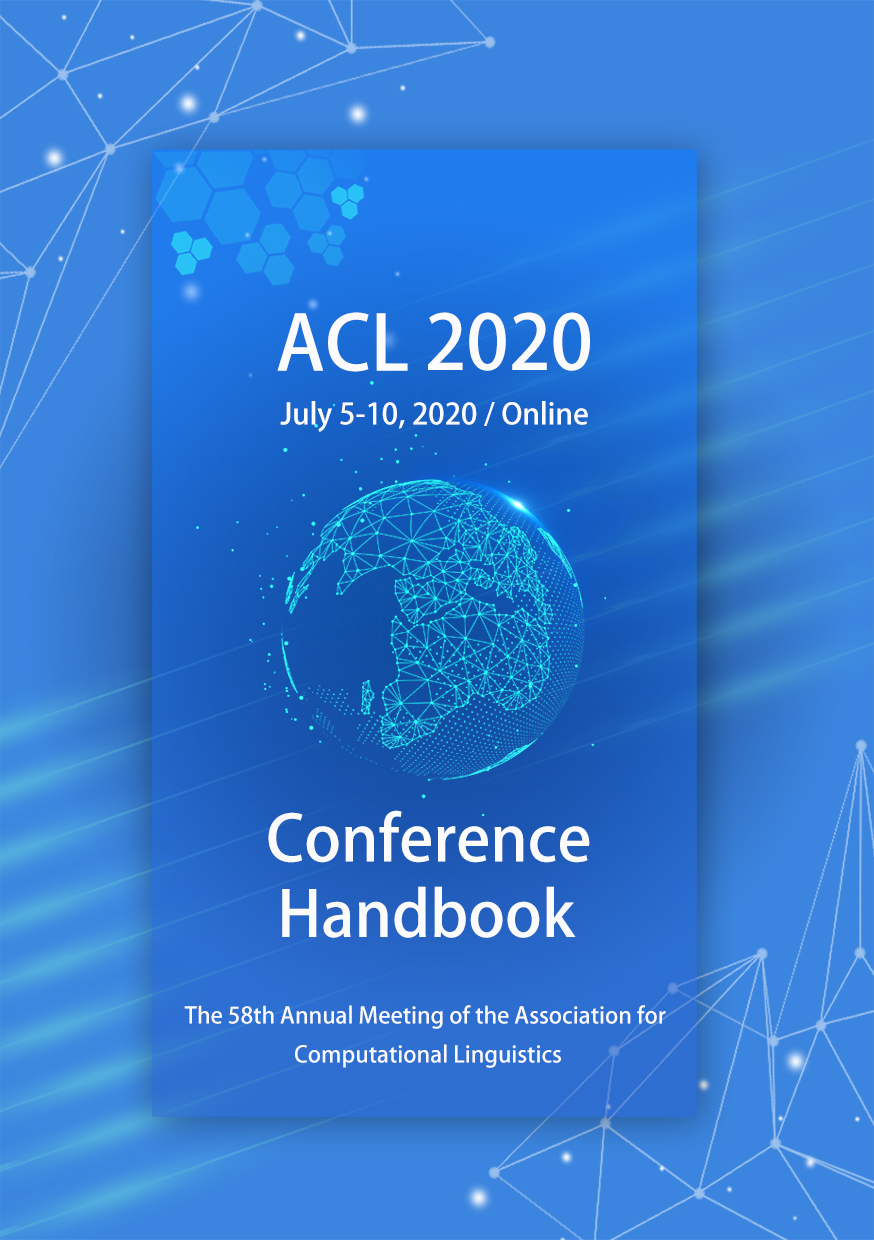
\includepdf[pages=1,%
%      pagecommand={%
%      {\LARGE TOREPLACE_TIMEZONE}
% }]{content/fmatter/cover.jpg}

%% INSIDE FRONT COVER %%%%%%%%%%%%%%%%%%%%%%%%%%%%%%%%%%%%%%%%%%%

%TODO: add one page conference overview

%\cleardoublepage
\thispagestyle{empty}

% \resizebox{\textwidth}{!}{
\newcommand{\daywidth}{2.2 cm}
\begin{tikzpicture}[x=\daywidth, y=-1cm, node distance=0 cm,outer sep = 0pt]
% Style for Days
\tikzstyle{day}=[draw, rectangle,  minimum height=1cm, minimum width=\daywidth, fill=yellow!20,anchor=south west]
% Style for hours
\tikzstyle{hour}=[draw, rectangle, minimum height=1 cm, minimum width=1.5 cm, fill=yellow!30,anchor=north east]
\tikzstyle{hourr}=[draw, rectangle, minimum height=1 cm, minimum width=1.5 cm, fill=yellow!30,anchor=north west]
% Styles for events
% Duration of sequences
\tikzstyle{hours}=[rectangle,draw, minimum width=\daywidth, anchor=north west,text centered,text width=5 em]
\tikzstyle{1hour}=[hours,minimum height=1cm]
\tikzstyle{2hours}=[hours,minimum height=2cm]
\tikzstyle{3hours}=[hours,minimum height=3cm]
%Style for type of sequence 
\tikzstyle{Ang2h}=[2hours,fill=green!20]
\tikzstyle{Phys2h}=[2hours,fill=red!20]
\tikzstyle{Math2h}=[2hours,fill=blue!20]
\tikzstyle{TIPE2h}=[2hours,fill=blue!10]
\tikzstyle{TP2h}=[2hours, pattern=north east lines, pattern color=magenta]
\tikzstyle{G3h}=[3hours, pattern=north west lines, pattern color=magenta!60!white]
\tikzstyle{Planche}=[1hour,fill=white]
% Positioning labels for days and hours
\node[day] (sun) at (1,8) {Sun 15};
\node[day] (mon) [right = of sun] {Mon 16};
\node[day] (tue) [right = of mon] {Tue 17};
\node[day] (wed) [right = of tue] {Wed 18};
\node[day] (thu) [right = of wed] {Thu 19};
\node[day] (fri) [right = of thu] {Fri 20};
\node[hour] (8-9) at (1,8) {8-9};
\node[hour] (9-10) [below = of 8-9] {9-10};
\node[hour] (10-11) [below= of 9-10] {10-11};
\node[hour] (11-12) [below = of 10-11] {11-12};
\node[hour] (12-13) [below  = of 11-12] {12-13};
\node[hour] (13-14) [below = of 12-13] {13-14};
\node[hour] (14-15) [below = of 13-14] {14-15};
\node[hour] (15-16) [below = of 14-15] {15-16};
\node[hour] (16-17) [below = of 15-16] {16-17};
\node[hour] (17-18) [below = of 16-17] {17-18};
\node[hour] (18-19) [below = of 17-18] {18-19};
\node[hour] (19-20) [below = of 18-19] {19-20};
\node[hour] (20-21) [below = of 19-20] {20-21};
\node[hour] (21-22) [below = of 20-21] {21-22};
\node[hour] (22-23) [below = of 21-22] {22-23};
%
\node[hourr] (8-9) at (7,8) {8-9};
\node[hourr] (9-10) [below = of 8-9] {9-10};
\node[hourr] (10-11) [below= of 9-10] {10-11};
\node[hourr] (11-12) [below = of 10-11] {11-12};
\node[hourr] (12-13) [below  = of 11-12] {12-13};
\node[hourr] (13-14) [below = of 12-13] {13-14};
\node[hourr] (14-15) [below = of 13-14] {14-15};
\node[hourr] (15-16) [below = of 14-15] {15-16};
\node[hourr] (16-17) [below = of 15-16] {16-17};
\node[hourr] (17-18) [below = of 16-17] {17-18};
\node[hourr] (18-19) [below = of 17-18] {18-19};
\node[hourr] (19-20) [below = of 18-19] {19-20};
\node[hourr] (20-21) [below = of 19-20] {20-21};
\node[hourr] (21-22) [below = of 20-21] {21-22};
\node[hourr] (22-23) [below = of 21-22] {22-23};
%Position of sequences
\node[hours,minimum height=1.5cm,fill=pink!20] at (1,9) {Tutorials};
\node[Planche,minimum height=0.5cm] at (1,10.5) {Coffee};
\node[hours,minimum height=1.5cm,fill=pink!20] at (1,11) {Tutorials};
\node[Planche] at (1,12.5) {Lunch};
\node[hours,minimum height=1.5cm,fill=pink!20] at (1,13.5) {Tutorials};
\node[Planche,minimum height=0.5cm] at (1,15) {Coffee};
\node[hours,minimum height=1.5cm,fill=pink!20] at (1,15.5) {Tutorials};
\node[hours,minimum height=2cm,fill=blue!20] at (1,18) {Welcome Reception};
%
\node[hours,minimum height=1cm,fill=red!20] at (2,9) {Welcome; President};
\node[Planche,minimum height=0.5cm] at (2,10) {Coffee};
\node[hours,minimum height=1.667cm,fill=green!20] at (2,10.5) {Talks 1};
\node[hours,minimum height=1.5cm,fill=cyan!20] at (2,12.5) {Poster 1, Demo 1};
\node[hours,minimum height=1.667cm,fill=green!20] at (2,14) {Talks 2};
\node[Planche,minimum height=0.5cm] at (2,15.667) {Coffee};
\node[hours,minimum height=1.667cm,fill=green!20] at (2,16.1667) {Talks 3};
\node[hours,minimum height=1.5cm,fill=blue!20] at (2,18.25) {Student Recruitment};
%
\node[hours,minimum height=1cm,fill=red!20] at (3,9) {Keynote Ros\'{e}};
\node[Planche,minimum height=0.5cm] at (3,10) {Coffee};
\node[hours,minimum height=1.667cm,fill=green!20] at (3,10.5) {Talks 4};
\node[hours,minimum height=1.5cm,fill=cyan!20] at (3,12.5) {Poster 2, Demo 2};
\node[hours,minimum height=1cm,fill=green!10] at (3,14) {Talks 5};
\node[Planche,minimum height=0.5cm] at (3,15) {Coffee};
\node[hours,minimum height=1.667cm,fill=green!20] at (3,15.5) {Talks 6};
\node[hours,minimum height=1.5cm,fill=red!20] at (3,17.3333) {Business};
\node[hours,minimum height=3cm,fill=blue!20] at (3,19.5) {Social (Acquarium)};
%
\node[hours,minimum height=1cm,fill=red!20] at (4,9) {Keynote van den Bosch};
\node[Planche,minimum height=0.5cm] at (4,10) {Coffee};
\node[hours,minimum height=1.667cm,fill=green!20] at (4,10.5) {Talks 7};
\node[hours,minimum height=1.5cm,fill=cyan!20] at (4,12.5) {Poster 3, Demo 3};
\node[hours,minimum height=1cm,fill=green!10] at (4,14) {Talks 8};
\node[Planche,minimum height=0.5cm] at (4,15) {Coffee};
\node[hours,minimum height=1.75cm,fill=green!20] at (4,15.5) {Best papers};
\node[hours,minimum height=1.25cm,fill=red!20] at (4,17.5) {Lifetime A.A.; Closing};
%\node[hours,minimum height=0.25cm,fill=red!20] at (4,18.5) {Closing};
%
\node[hours,minimum height=9.25cm,fill=orange!30] at (5,8.75) {};
\node[hours,minimum height=1.75cm,fill=orange!30] at (5,8.75) {Workshops$^{\dagger}$};
\node[Planche,minimum height=0.5cm] at (5,10.50) {Coffee};
\node[Planche,minimum height=1cm] at (5,12.50) {Lunch$^{\dagger}$};
\node[Planche,minimum height=0.5cm] at (5,15.50) {Coffee};
%
\node[hours,minimum height=9.25cm,fill=orange!30] at (6,8.75) {Workshops$^{\dagger}$};
\node[hours,minimum height=1.75cm,fill=orange!30] at (6,8.75) {Workshops$^{\dagger}$};
\node[Planche,minimum height=0.5cm] at (6,10.50) {Coffee};
\node[Planche,minimum height=1cm] at (6,12.50) {Lunch$^{\dagger}$};
\node[Planche,minimum height=0.5cm] at (6,15.50) {Coffee};
\end{tikzpicture}
}
\emph{$\dagger$: Start, end and lunch times vary between workshops, the above is a rough guide.}


\vspace*{15.3em}
\noindent\emph{Handbook assembled by \href{https://vnpeng.net}{Nanyun Violet Peng} and \href{https://mingyu.ma}{Mingyu Derek Ma}}\\\index{Peng, Nanyun} 
\index{Ma, Mingyu Derek}

\noindent\emph{Cover designed by \href{https://jingyachen.net}{Jingya Chen}}\\\index{Chen, Jingya}

\newpage
\cleardoublepage
\fancyfoot[C]{\thepage}
\frontmatter

%% SPONSORS %%%%%%%%%%%%%%%%%%%%%%%%%%%%%%%%%%%%%%%%%%%%%%%%%%%%%

%% Putting on back cover

%% \addcontentsline{toc}{chapter}{Sponsorship}
%% \thispagestyle{empty}
%% \setheaders{}{}
%% 
Diamond Sponsors:\\

\begin{tabular}{ c c c }
\raisebox{-0.5\height}{
\includegraphics[width=2cm]{content/sponsors/logos/google.png}} & \raisebox{-0.5\height}{
\includegraphics[width=2cm]{content/sponsors/logos/bytedance-toutiao.png}} & \raisebox{-0.5\height}{
\includegraphics[width=2cm]{content/sponsors/logos/samsung.jpg}} \\ 
\raisebox{-0.5\height}{
\includegraphics[width=2cm]{content/sponsors/logos/Apple_Logo_429C_RGB_090318_clearspace.pdf}} & 
\raisebox{-0.5\height}{
\includegraphics[width=2cm]{content/sponsors/logos/facebook.png}} & 
\end{tabular}
\\

%
\includegraphics[width=3.5cm]{content/sponsors/logos/google.png}\qquad
%
\includegraphics[width=3.5cm]{content/sponsors/logos/bytedance-toutiao.png}\qquad
%
\includegraphics[width=3.5cm]{content/sponsors/logos/samsung.jpg}\\%\qquad
%
\includegraphics[width=3.5cm]{content/sponsors/logos/Apple_Logo_429C_RGB_090318_clearspace.pdf}\qquad
%
\includegraphics[width=3.5cm]{content/sponsors/logos/facebook.png}\\

Platinum Sponsors:\\

\begin{tabular}{ c c c }
	\raisebox{-0.5\height}{
\includegraphics[width=3.2cm]{content/sponsors/logos/amazon.png}} & \raisebox{-0.5\height}{
\includegraphics[width=3.5cm]{content/sponsors/logos/baidu.png}} & \raisebox{-0.5\height}{
\includegraphics[width=3.5cm]{content/sponsors/logos/jingdong.png}} \\ 
	&&\\
	\raisebox{-0.5\height}{
\includegraphics[width=3.5cm]{content/sponsors/logos/rit.png}} & 
	\raisebox{-0.5\height}{
\includegraphics[width=3.5cm]{content/sponsors/logos/tencent.png}} & \\
\end{tabular}
\\
\\
\\

%
\includegraphics[width=3.1cm]{content/sponsors/logos/amazon.png}\qquad
%
\includegraphics[width=3.4cm]{content/sponsors/logos/baidu.png}\qquad
%
\includegraphics[width=3.4cm]{content/sponsors/logos/jingdong.png}\qquad
%
\includegraphics[width=3.4cm]{content/sponsors/logos/rit.png}\qquad
%
\includegraphics[width=3.5cm]{content/sponsors/logos/tencent.png}\\

Gold Sponsors:\\

\begin{tabular}{ c c c }
	\raisebox{-0.5\height}{\LARGE \bf IBM Research} & \raisebox{-0.5\height}{
\includegraphics[width=4cm]{content/sponsors/logos/microsoft.png}} & \raisebox{-0.5\height}{
\includegraphics[width=3.9cm]{content/sponsors/logos/naver.png}} \\
	&&\\
	\raisebox{-0.5\height}{
\includegraphics[width=3.9cm]{content/sponsors/logos/cvte.jpg}} & 
	\raisebox{-0.5\height}{
\includegraphics[width=4.5cm]{content/sponsors/logos/dhcrc.jpg}} & 
\end{tabular}
\\
\\
\\

%IBM Research\qquad 
%
\includegraphics[width=3.6cm]{content/sponsors/logos/microsoft.png}\qquad
%
\includegraphics[width=3.6cm]{content/sponsors/logos/naver.png}\qquad
%
\includegraphics[width=3.6cm]{content/sponsors/logos/cvte.jpg}\\

Silver Sponsors:\\

\begin{tabular}{ c c c c }
	\raisebox{-0.5\height}{
\includegraphics[width=3.5cm]{content/sponsors/logos/nuance.png}}\quad & 
	\raisebox{-0.5\height}{
\includegraphics[width=2.1cm]{content/sponsors/logos/huawei.png}}\quad\quad & 
	\raisebox{-0.5\height}{
\includegraphics[width=2.1cm]{content/sponsors/logos/elsevier.png}}\quad &
	\raisebox{-0.5\height}{
\includegraphics[width=3.5cm]{content/sponsors/logos/duolingo-cropped.jpg}} \\
\end{tabular}


%
\includegraphics[width=3.6cm]{content/sponsors/logos/nuance.png}\qquad\qquad
%
\includegraphics[width=2cm]{content/sponsors/logos/huawei.png}\qquad\qquad
%
\includegraphics[width=2cm]{content/sponsors/logos/elsevier.png}\qquad\qquad
%
\includegraphics[width=3.7cm]{content/sponsors/logos/duolingo.jpg}
%\qquad
%%
\includegraphics[width=3.5cm]{content/sponsors/logos/tencent.png}\\

\newpage

Bronze Sponsors:\\

%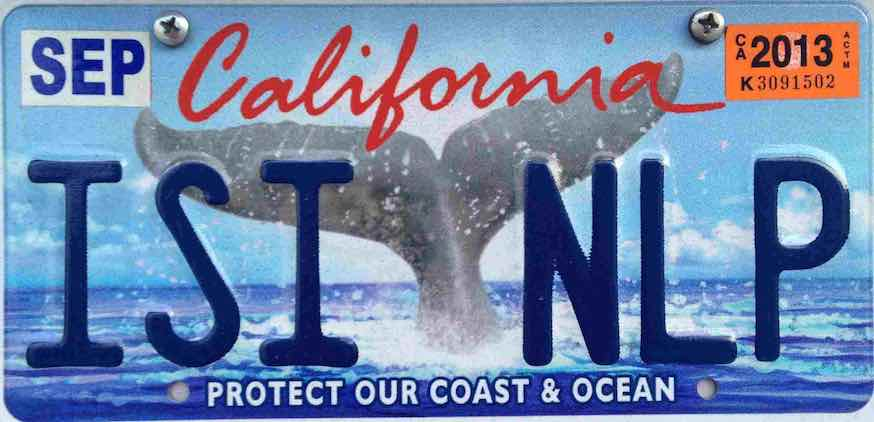
\includegraphics[width=3.6cm]{content/sponsors/logos/isi-nlp.jpg}\qquad 

\begin{tabular}{ c c }
	\raisebox{-0.5\height}{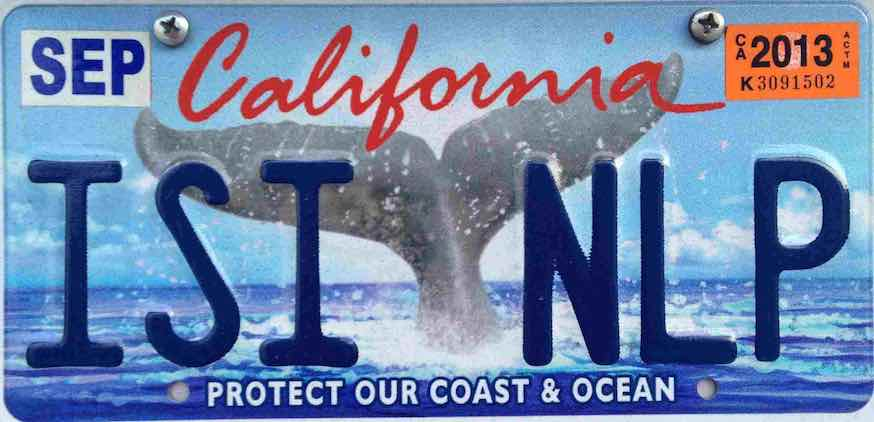
\includegraphics[width=3.5cm]{content/sponsors/logos/isi-nlp.jpg}}\quad\quad & \raisebox{-0.5\height}{
\includegraphics[width=6.5cm]{content/sponsors/logos/dstg.pdf}}\quad\quad \\
\end{tabular}
\\
\\

%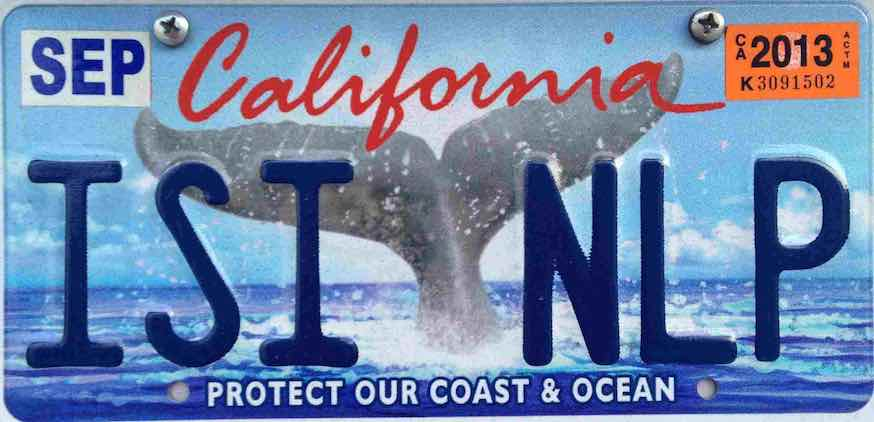
\includegraphics[width=3.6cm]{content/sponsors/logos/isi-nlp.jpg}\qquad 
%\includegraphics[width=3.6cm]{content/sponsors/logos/DSTGroup-Logo-Vert.jpg}

Supporters: \\

\begin{tabular}{ c c }
	\raisebox{-0.5\height}{
\includegraphics[width=3.5cm]{content/sponsors/logos/roam.png}}\quad\quad & \raisebox{-0.5\height}{
\includegraphics[width=3.5cm]{content/sponsors/logos/sap.png}}\quad\quad \\
\end{tabular}
\\
\\

%
\includegraphics[width=3.5cm]{content/sponsors/logos/roam.png} \qquad
%
\includegraphics[width=3.5cm]{content/sponsors/logos/sap.png}\\

Student Volunteers Sponsors: \\

\quad\enskip\includegraphics[width=3.5cm]{content/sponsors/logos/data61.png}


%% TOC %%%%%%%%%%%%%%%%%%%%%%%%%%%%%%%%%%%%%%%%%%%%%%%%%%%%%%%%%%

\addcontentsline{toc}{chapter}{Table of Contents}
\setcounter{tocdepth}{1}
\tableofcontents
\mainmatter
\pagestyle{fancy}

%% PREFACE %%%%%%%%%%%%%%%%%%%%%%%%%%%%%%%%%%%%%%%%%%%%%%%%%%%%%%

\chapter{Conference Information}

\section{Message from the General Chair}\vspace{2em}
\setheaders%
    {Message from the General Chair}%
    {Message from the General Chair}
\thispagestyle{emptyheader}
\begin{large}
\setlength{\parskip}{1ex}

\noindent Welcome to ACL 2014!

I remember with great fondness the first ACL Conference I attended 20 years ago in Las Cruces, New Mexico. Some things have changed: papers presented there that I considered interesting or inconsequential have switched positions in my personal ranking as I learned more and more about our field; single sessions have long been replaced by parallel sessions to accommodate an ever increasing number of research contributions; the number of associated workshops and posters has mushroomed beyond anyone's dream. Almost without noticing, we transitioned from small conferences of a few hundred to conferences that bring together 1000 plus participants from all over the world.  Our field has matured significantly attracting the attention of not only a handful of academics, but successful industries and Research Labs as well.  Some things have stayed the same though: ACL continues to be the pre-eminent conference in our field and the best place to meet and make like-minded friends, discuss tantalizing tricks that you can learn about only in face-to-face communication settings, and celebrate the results we get.

On behalf of the organizing committee, I welcome you to the conference; make the most of it!

\vspace{.2in}
Daniel Marcu \\
\indent General Chair
\end{large}

\index{Marcu, Daniel}

\clearpage
\section{Message from the Program Committee Co-Chairs}
\setheaders%
    {Message from the Program Committee Co-Chairs}%
    {Message from the Program Committee Co-Chairs}
\thispagestyle{emptyheader}
%\renewcommand{\large}{\fontsize{9}{11}\selectfont}
% that's a hack to make this part nicely fill the pages

\setlength{\parskip}{.7ex}
%\setlength{\parindent}{0pt}

Welcome to the 2015 Conference of the North American Chapter of the
Association for Computational Linguistics -- Human Language
Technologies or NAACL HLT 2015 for short. 

This year, we received the largest number of submissions in the
history of NAACL: a total of 714 submissions with 402 long paper
submissions and 312 short papers submissions. From these, 117 long
papers (62 oral presentations and 55 poster presentations) and 69
short papers (24 oral presentations and 45 poster presentations)
were accepted to appear at the conference.

The submissions to NAACL HLT 2015 were assigned to 18 technical
areas including a new topic area called {\em Language and Vision}.
This track was introduced with an intent to broaden research on
natural language processing that is situated in a rich visual and
perceptual context. We received 16 submissions for this area and
seven of them will be presented at the conference.

For NAACL HLT 2015 we initiated a meta review process, where each
paper received an analysis of the merits of the paper from the area
chair's perspective that was based on the reviewer comments, the
reviewer discussion and the author rebuttal.  We found the meta
reviews very helpful in consolidating the reviews and providing
justifications for final decisions. As this was an experiment this
year, the meta reviews were not sent to the authors.

Based on comments from reviewers, nominations from area chairs, and
rankings from the best paper committee, three papers were selected
to receive the best paper awards at the conference.

Continuing the tradition, NAACL HLT 2015 will feature 19 papers
which were accepted for publication in the Transactions of the
Association for Computational Linguistics (TACL). The TACL papers
were split into 10 oral presentations and 9 poster presentatons.

We are very pleased to have two exciting keynote talks: one by
Professor Lillian Lee (Cornell University) and the other by Professor
Fei-Fei Li (Stanford University).

There are many people to thank for who have worked diligently to
make NAACL HLT 2015 possible. Thanks to the 32 area chairs
for their hard work on recruiting reviewers, managing reviews,
leading discussions, and making recommendations.  All the area
chairs are listed in the Program Committee section of the Front
Matter.  Thanks to Chris Callison-Burch, David Mimno,
Sameer Pradhan, and Philip Resnik for stepping in to serve as area
co-chairs at the last minute when we were faced with an unexpectedly
large number of submissions in some tracks.

Following what was done in the last NAACL conference, we used the
paper assignment tool developed by Mark Dredze to assign papers to
reviewers.  Thanks to Mark Dredze and Jiang Guo for
their hard work on assigning papers to reviewers based on their
preferences.  We had to especially rely on this tool this year
because the distribution of submissions across areas was very
different from past trends.

This program certainly would not be possible without the help of
the 460 reviewers. Their names are listed in the Program Committee
section.  In particular, 116 reviewers from this list were recognized
by the area chairs as best reviewers who have turned in exceptionally
well-written and constructive reviews and who have actively engaged in
the post-rebuttal discussions. The names of the best reviewers are
marked with * in the list of reviewers. 

We are also indebted to the best paper award committee which consists
of Claire Cardie, Daniel Gildea, Daniel Marcu, and Fernando Pereira.
Their time and effort in recommending the best paper awards is much
appreciated.

We also would like to thank Hal Daum\'{e} III, Kristina Toutanova,
and Lucy Vanderwende for generously sharing their experience in
organizing prior NAACL/ACL conferences and for their advice. We are
grateful for the guidance and the support of the NAACL president
Hal Daum\'{e} III, and the NAACL board. We also would like to thank
the publication co-chairs Matt Post and Adam Lopez for putting
together the proceedings and the conference handbook; and Paolo Gai
and Rich Gerber from Softconf for always being responsive to our
requests. 

We would like to thank the ACL Business Manager Priscilla Rasmussen.
She was our {\em go to} person who knew all details of the conference
in and out.  We are very grateful for her help.

Finally, this conference could not have happened without the efforts
of the general chair, Rada Mihalcea. She made sure the various
sections of NAACL organization worked well together. Her monthly
newsletters informed all the organizers about what was being done
by everyone else. We are very thankful for her leadership in the
organization of NAACL HLT 2015.

We hope you will enjoy NAACL HLT 2015!

\noindent\includegraphics[scale=1.5]{content/fmatter/easteregg.pdf}

\noindent NAACL HLT 2015 Program Co-Chairs \\
Joyce Chai, Michigan State University \\
Anoop Sarkar, Simon Fraser University


\clearpage%{\thispagestyle{emptyheader}\cleardoublepage}
\setheaders{}{}
\markboth{}{} % clear the right header
\markright{}{} % clear the right header

\section{Organizing Committee}{}

\setlength{\parindent}{0pt}

{\bf General Chair} \\
Rada Mihalcea, University of Michigan, USA

{\bf Local Arrangements Chair} \\
Priscilla Rasmussen, ACL Business Manager

{\bf Program Committee Co-chairs} \\
Joyce Chai, Michigan State University, USA \\
Anoop Sarkar, Simon Fraser University, Canada

{\bf Workshop Co-chairs} \\
Cornelia Caragea, University of North Texas, USA \\
Bing Liu, University of Illinois at Chicago, USA

{\bf Tutorial Co-chairs} \\
Yang Liu, University of Texas at Dallas, USA \\
Thamar Solorio, University of Alabama at Birmingham, USA

{\bf Student Research Workshop Co-chairs} \\
\indent \emph{Student Co-chairs} \\
\hspace*{0.2in} Shibamouli Lahiri, University of Michigan, USA \\
\hspace*{0.2in} Karen Mazidi, University of North Texas, USA \\
\hspace*{0.2in} Alisa Zhila, Instituto Politécnico Nacional (National Polytechnic Institute), Mexico \\
\emph{Faculty Advisors} \\
\hspace*{0.2in} Diana Inkpen, University of Ottawa, Canada \\
\hspace*{0.2in} Smaranda Muresan, Columbia University, USA

{\bf Demo Co-chairs} \\
Matt Gerber, University of Virginia, USA \\
Catherine Havasi, Massachusetts Institute of Technology, USA \\
Finley Lacatusu, Language Computer Corporation, USA

{\bf Student Volunteer Coordinator} \\
Annie Louis, University of Edinburgh, UK

{\bf Reviewing Coordinators} \\
Mark Dredze, Johns Hopkins University \\
Jiang Guo, Harbin Institute of Technology

{\bf Local Sponsorship Chair} \\
Kevin B. Cohen, University of Colorado, USA

{\bf Publicity Chair} \\
Saif M. Mohammad, National Research Council Canada

{\bf Publication Co-chairs} \\
Matt Post, John Hopkins University, USA \\
Adam Lopez, University of Edinburgh, UK

{\bf Conference Handbook Editor} \\
Matt Post, Johns Hopkins University

{\bf Website Chair} \\
Peter Ljunglöf, University of Gothenburg and Chalmers University of Technology, Sweden

{\bf Business Manager} \\
Priscilla Rasmussen

%%%%%%%%%%%%%%%%%%%%%%%%%%%%%%%%%%%%%%%%%%%%%%%%%%%%%%%%%%%%%%%%%%%%%%%%

\clearpage
\section{Program Committee}
\setlength{\parindent}{0pt}

\vspace*{0.5cm}

{\bf Program Committee Co-chairs} \\
Joyce Chai, Michigan State University, USA \\
Anoop Sarkar, Simon Fraser University, Canada

{\bf Area Chairs} \\
\emph{Dialogue and Interactive Systems} \\
\hspace*{0.2in} Jason D. Williams, Microsoft Research

\emph{Discourse and Pragmatics} \\
\hspace*{0.2in} Ani Nenkova, University of Pennsylvania \\
\hspace*{0.2in} Vincent Ng, University of Texas at Dallas 

\emph{Generation and Summarization} \\
\hspace*{0.2in} Chris Callison-Burch, University of Pennsylvania \\
\hspace*{0.2in} Fei Liu, Carnegie Mellon University

\emph{Information Extraction and Question Answering} \\
\hspace*{0.2in} Alan Ritter, The Ohio State University \\
\hspace*{0.2in} Bowen Zhou, IBM Research

\emph{Information Retrieval} \\
\hspace*{0.2in} David Smith, Northeastern University

\emph{Language and Vision} \\
\hspace*{0.2in} Julia Hockenmaier, University of Illinois at Urbana-Champaign

\emph{Language Resources and Evaluation} \\
\hspace*{0.2in} Will Lewis, Microsoft Research \\
\hspace*{0.2in} Sameer Pradhan, Harvard University

\emph{Linguistic and Psycholinguistic Aspects of CL} \\
\hspace*{0.2in} William Schuler, The Ohio State University

\emph{Machine Learning for NLP} \\
\hspace*{0.2in} Amarnag Subramanya, Google Research \\
\hspace*{0.2in} Tong Zhang, Baidu Inc. and Rutgers University

\emph{Machine Translation} \\
\hspace*{0.2in} Bill Byrne, Cambridge University \\
\hspace*{0.2in} Hany Hassan, Microsoft Research \\
\hspace*{0.2in} Kevin Knight, Information Sciences Institute, University of Southern California \\
\hspace*{0.2in} Haitao Mi, IBM Research

\emph{NLP for Web, Social Media and Social Sciences} \\
\hspace*{0.2in} Brendan O'Connor, University of Massachusetts \\
\hspace*{0.2in} Philip Resnik, University of Maryland

\emph{NLP-enabled Technology} \\
\hspace*{0.2in} Richard Socher, Stanford University

\emph{Phonology, Morphology, and Word Segmentation} \\
\hspace*{0.2in} Sami Virpioja, Lingsoft and Aalto University

\emph{Semantics} \\
\hspace*{0.2in} Dipanjan Das, Google \\
\hspace*{0.2in} William Dolan, Microsoft Research \\
\hspace*{0.2in} Luke Zettlemoyer, University of Washington

\emph{Sentiment Analysis and Opinion Mining} \\
\hspace*{0.2in} Saif M. Mohammad, National Research Council Canada \\
\hspace*{0.2in} Jerry Zhu, University of Wisconsin-Madison

\emph{Spoken Language Processing} \\
\hspace*{0.2in} Xiaodong He, Microsoft Research

\emph{Tagging, Chunking, Syntax, and Parsing} \\
\hspace*{0.2in} Noah Smith, Carnegie Mellon University \\
\hspace*{0.2in} Yue Zhang, Singapore University of Technology and Design

\emph{Text Categorization and Topic Models} \\
\hspace*{0.2in} Jordan Boyd-Graber, University of Colorado at Boulder \\
\hspace*{0.2in} David Mimno, Cornell University


\clearpage

%% TUTORIALS %%%%%%%%%%%%%%%%%%%%%%%%%%%%%%%%%%%%%%%%%%%%%%%%%%%%

% \setdaydateyear{Sunday}{July 5}{2020}
% \chapter{Tutorials: \daydate}
\thispagestyle{emptyheader}
\setheaders{Tutorials}{\daydateyear}
\setlength{\parindent}{0in}
\setlength{\parskip}{2ex}
\renewcommand{\baselinestretch}{0.87}

\newcommand{\tutorialmorningtime}{9:00--12:00pm}
\newcommand{\tutorialafternoontime}{2:00--5:00pm}

\section*{Overview}
\renewcommand{\arraystretch}{1.2}
\begin{SingleTrackSchedule}
  7:30 & -- & 6:00 &
  {\bfseries Registration} \hfill (\RegistrationLoc)
  \\
  7:30 & -- & 9:00 &
  {\bfseries Breakfast} \hfill (\BreakfastLoc)
  \\
  9:00 & -- & 12:00 &
  {\bfseries Morning Tutorials} \hfill
  \\
  & & & \papertitle{tutorial-final-014}\hfill (\TutLocA)\newline
  \tutorialauthors{tutorial-final-014} \\
  \\
  & & & \papertitle{tutorial-final-021}\hfill (\TutLocB)\newline
  \tutorialauthors{tutorial-final-021} \\
  \\
  & & & \papertitle{tutorial-final-025}\hfill (\TutLocC)\newline
  \tutorialauthors{tutorial-final-025} \\
  \\
  12:00 & -- & 2:00 &
  {\bfseries Lunch break}
  \\
  2:00 & -- & 5:00 &
  {\bfseries Afternoon Tutorials} \hfill
  \\
  & & & \papertitle{tutorial-final-019}\hfill (\TutLocE)\newline
  \tutorialauthors{tutorial-final-019} \\
  \\
  & & & \papertitle{tutorial-final-009}\hfill (\TutLocF)\newline
  \tutorialauthors{tutorial-final-009} \\
  \\
  & & & \papertitle{tutorial-final-022}\hfill (\TutLocG)\newline
  \tutorialauthors{tutorial-final-022} \\
  \\
  6:00 & -- & 9:00 &
  {\bfseries Welcome Reception} \hfill (\WelcomeReceptionLoc)
  \\
\end{SingleTrackSchedule}

\clearpage\begin{bio}
  {\bfseries Hal Daumé III} is an associate professor in Computer Science at the University of Maryland, College Park. He holds joint appointments in UMIACS and Linguistics. His primary research interest is in developing new learning algorithms for prototypical problems that arise in the context of language processing and artificial intelligence. This includes topics like structured prediction, domain adaptation and unsupervised learning; as well as multilingual modeling and affect analysis.

  {\bfseries John Langford} is a machine learning research scientist. He is the author of the blog hunch.net and the principal developer of Vowpal Wabbit. John works at Microsoft Research New York, of which he was one of the founding members, and was previously affiliated with Yahoo! Research, Toyota Technological Institute, and IBM’s Watson Research Center. He studied Physics and Computer Science at the California Institute of Technology, earning a double bachelor’s degree in 1997, and received his Ph.D. in Computer Science from Carnegie Mellon University in 2002. He was the program co-chair for the 2012 International Conference on Machine Learning.

  {\bfseries Kai-Wei Chang} is a doctoral candidate in Computer Science at the University of Illinois at Urbana-Champaign. His research interests lie in designing practical machine learning techniques for large and complex data and applying them to real world applications. He has been working on various topics in Machine learning and Natural Language Processing, including large-scale learning, structured learning, coreference resolution, and relation extraction.

  {\bfseries He He} is a doctoral student in Computer Science at the University of
  Maryland, College Park. Her research interests focus on developing
  fast inference methods for structured prediction problems in machine
  learning and natural language processing, including features
  selection, dependency parsing and machine translation.

  {\bfseries Sudha Rao} is a doctoral student in Computer Science at the University of Maryland, College Park. Her research interests currently lie in exploring how semantic representations like Abstract Meaning Representation can be used in Machine Translation.
  
\end{bio}

\begin{tutorial}
  {Hands-on Learning to Search for Structured Prediction}
  {tutorial-final-014}
  {\daydateyear, \tutorialmorningtime}
  {\TutLocA}

Many problems in natural language processing involve building outputs that are structured. The predominant approach to structured prediction is ``global models'' (such as conditional random fields), which have the advantage of clean underlying semantics at the cost of computational burdens and extreme difficulty in implementation. An alternative strategy is the ``learning to search'' (L2S) paradigm, in which the structured prediction task is cast as a sequential decision making process. One can then devise training-time algorithms that learn to make near optimal collective decisions. This paradigm has been gaining increasing traction over the past five years: most notably in dependency parsing (e.g., MaltParser, ClearNLP, etc.), but also much more broadly in less ``sequential'' tasks like entity/relation classification and even graph prediction problems found in social network analysis and computer vision.

This tutorial has precisely one goal: an attendee should leave the tutorial with hands on experience writing small programs to perform structured prediction for a variety of tasks, like sequence labeling, dependency parsing and, time-permitting, more.

This proposed tutorial is unique (to our knowledge) among ACL tutorials in this regard: half of the time spent will be in the style of a ``flipped classroom'' in which attendees get hands on experience writing structured predictors on their own or in small groups. All course materials (software, exercises, hints, solutions, etc., will be made available at least two weeks prior to the event so that students can download the required data ahead of time; we will also bring copies on USB in case there is a problem with the internet).

The first half of the tutorial will be mostly ``lecture'' style, in which we will cover the basics of how learning to search works for structured prediction. The goal is to provide enough background information that students can understand how to write and debug their own predictors, but the emphasis will not be on how to build new machine learning algorithms. This will also include a brief tutorial on the basics of Vowpal Wabbit, to the extent necessary to understand its structured prediction interface. The second half of the tutorial will focus on hands-on exploration of structured prediction using the Vowpal Wabbit python ``learning to search'' interface; a preliminary python notebook explaining the interface can be viewed at \url{http://tinyurl.com/pyvwsearch}; an elaborated version of this notebook will serve as the backbone for the ``hands on'' part of the tutorial, paired with exercises.

\end{tutorial}

\clearpage\begin{tutorial}
  {Neural Approaches to Conversational AI}
  {tutorial-026}
  {\daydateyear, \tutorialmorningtime}
  {\TutLocB}
\end{tutorial}

This tutorial surveys neural approaches to conversational AI that were developed in the last few years. We group conversational systems into three categories: (1) question answering agents, (2) task-oriented dialogue agents, and (3) social bots. For each category,  we present a review of state-of-the-art neural approaches, draw the connection between neural approaches and traditional symbolic approaches, and discuss the progress we have made and challenges we are facing, using specific systems and models as case studies.


\vspace{2ex}\centerline{\rule{.5\linewidth}{.5pt}}\vspace{2ex}
\setlength{\parskip}{1ex}\setlength{\parindent}{0ex}




{\bfseries Jianfeng Gao} is Partner Research Manager at Microsoft
AI and Research, Redmond. He leads the
development of AI systems for machine reading
comprehension, question answering, chitchat bots,
task-oriented dialogue, and business applications.
From 2014 to 2017, he was Partner Research Manager
and Principal Researcher at Deep Learning
Technology Center at Microsoft Research, Redmond,
where he was leading the research on deep
learning for text and image processing. From
2006 to 2014, he was Researcher, Senior Researcher,
and Principal Researcher at Natural Language
Processing Group at Microsoft Research,
Redmond, where he worked on the Bing search
engine, improving its core relevance engine and
query spelling, understanding and reformulation
engines, MS ads relevance and prediction, and statistical
machine translation. From 2005 to 2006,
he was a Research Lead in Natural Interactive Services
Division at Microsoft, where he worked on
Project X, an effort of developing natural user interface
for Windows. From 2000 to 2005, he was
Research Lead in Natural Language Computing
Group at Microsoft Research Asia, where he and
his colleagues developed the first Chinese speech
recognition system released with Microsoft Office,
the Chinese/Japanese Input Method Editors (IME)
which were the leading products in the market, and
the natural language platform for Microsoft Windows.

{\bfseries Michel Galley} is a Senior Researcher at Microsoft
Research. His research interests are in
the areas of natural language processing and machine
learning, with a particular focus on conversational
AI, text generation, and machine translation.
From 2007 to 2010, he was a Postdoctoral
Scholar then Research Associate in the Computer
Science department at Stanford University, working
primarily on Machine Translation. In 2007,
he obtained his Ph.D. from the Computer Science
department at Columbia University, with research
focusing on summarization, discourse, and dialogue.
From 2003 to 2005, he did several internships
at USC/ISI and Language Weaver on machine
translation, which included work that won
several NIST MT competitions. From 2000-2001,
he did an 8-month internship and undergraduate
thesis work in the Spoken Dialog Systems group
at Bell Labs, working on generation for dialogue
systems.

{\bfseries Lihong Li} is a Research Scientist at Google
Inc. He obtained a PhD degree in Computer Science
from Rutgers University, specializing in reinforcement
learning theory and algorithms. After
that, he has held Researcher, Senior Researcher,
and Principal Researcher positions in Yahoo!
Research (2009-2012) and Microsoft Research
(2012-2017), before joining Google. His
main research interests are reinforcement learning
(in both Markov decision processes and contextual
bandits) and other related problems in AI (including
active leaning, online learning and large-scale
machine learning). His work has found applications
in recommendation, advertising, Web search
and conversation systems, and has won best paper
awards at ICML, AISTATS and WSDM. In recent
years, he served as area chairs or senior program
committee members at AAAI, AISTATS, ICML,
IJCAI and NIPS. More information can be found
on his homepage: \url{http://lihongli.github.io}.





\clearpage\begin{tutorial}
  {Variational Inference and Deep Generative Models}
  {tutorial-027}
  {\daydateyear, \tutorialmorningtime}
  {\TutLocC}
\end{tutorial}

NLP has seen a surge in neural network models in recent years. These models
provide state-of-the-art performance on many supervised tasks. Unsupervised and
semi-supervised learning has only been addressed scarcely, however. Deep
generative models (DGMs) make it possible to integrate neural networks with
probabilistic graphical models. Using DGMs one can easily design latent
variable models that account for missing observations and thereby enable
unsupervised and semi-supervised learning with neural networks. The method of
choice for training these models is variational inference.

This tutorial offers a general introduction to variational inference followed
by a thorough and example-driven discussion of how to use variational methods
for training DGMs. It provides both the mathematical background necessary for
deriving the learning algorithms as well as practical implementation
guidelines.  Importantly, the tutorial will cover models with continuous and
discrete variables. 

We provide practical coding exercises implemented in IPython notebooks as well
as short notes on the more intricate mathematical details that the audience can
use as a reference after the tutorial. We expect that with these additional
materials the tutorial will have a long-lasting impact on the community.


\vspace{2ex}\centerline{\rule{.5\linewidth}{.5pt}}\vspace{2ex}
\setlength{\parskip}{1ex}\setlength{\parindent}{0ex}


{\bfseries Wilker Aziz} is a research associate at the University
of Amsterdam (UvA) working on natural
language processing problems such as machine
translation, textual entailment, and paraphrasing.
His research interests include statistical
learning, probabilistic models, and methods
for approximate inference. Before joining UvA,
Wilker worked on exact sampling and optimisation
for statistical machine translation at the University
of Sheffield (UK) and at the University of
Wolverhampton (UK) where he obtained his PhD.
Wilker’s background is in Computer Engineering
which he studied at the Engineering School of the
University of S\~ao Paulo (Brazil).

{\bfseries Philip Schulz} is an applied scientist at Amazon
Research. Before joining Amazon, Philip did his
PhD at the University of Amsterdam. During the
last months of his PhD trajectory, he visited the
University of Melbourne. Philip’s background is
in Linguistics which he studied at the University
of T\"ubingen and UCL in London. These days, his
research interests revolve around statistical learning.
He has worked on Bayesian graphical models
for machine translation. More recently he has
extended this line of work towards deep generative
models. More broadly, Philip is interested
in probabilistic modeling, approximate inference
methods and statistical theory.



\clearpage\begin{tutorial}
  {Connecting Language and Vision to Actions}
  {tutorial-020}
  {\daydateyear, \tutorialmorningtime}
  {\TutLocD}
\end{tutorial}


A long-term goal of AI research is to build intelligent agents that can see the
rich visual environment around us, communicate this understanding in natural
language to humans and other agents, and act in a physical or embodied
environment. To this end, recent advances at the intersection of language and
vision have made incredible progress -- from being able to generate natural
language descriptions of images/videos, to answering questions about them, to
even holding free-form conversations about visual content! However, while these
agents can passively describe images or answer (a sequence of) questions about
them, they cannot act in the world (what if I cannot answer a question from my
current view, or I am asked to move or manipulate something?). Thus, the
challenge now is to extend this progress in language and vision to embodied
agents that take actions and actively interact with their visual environments.
To reduce the entry barrier for new researchers, this tutorial will provide an
overview of the growing number of multimodal tasks and datasets that combine
textual and visual understanding. We will comprehensively review existing
state-of-the-art approaches to selected tasks such as image captioning, visual
question answering (VQA) and visual dialog, presenting the key architectural
building blocks (such as co-attention) and novel algorithms (such as
cooperative/adversarial games) used to train models for these tasks. We will
then discuss some of the current and upcoming challenges of combining language,
vision and actions, and introduce some recently-released interactive 3D
simulation environments designed for this purpose.


\vspace{2ex}\centerline{\rule{.5\linewidth}{.5pt}}\vspace{2ex}
\setlength{\parskip}{1ex}\setlength{\parindent}{0ex}



{\bfseries Peter Anderson} is a final year PhD candidate in
Computer Science at the Australian National University,
supervised by Dr Stephen Gould, and a researcher
within the Australian Centre for Robotic
Vision (ACRV). His PhD focuses on deep learning
for visual understanding in natural language.
He was an integral member of the team that won
first place in the 2017 Visual Question Answering
(VQA) challenge at CVPR, and he has made
several contributions in image captioning, including
achieving first place on the COCO leaderboard
in July 2017. He has published at CVPR,
ECCV, EMNLP and ICRA, and spent time at numerous
universities and research labs including
Adelaide University, Macquarie University, and
Microsoft Research. His research is currently
focused on vision-and-language understanding in
complex 3D environments.

{\bfseries Abhishek Das} is a Computer Science PhD student
at Georgia Institute of Technology, advised
by Dhruv Batra, and working closely with Devi
Parikh. He is interested in deep learning and its
applications in building agents that can see (computer
vision), think (reasoning and interpretability),
talk (language modeling) and act (reinforcement
learning). He is a recipient of an Adobe Research
Fellowship and a Snap Research Fellowship.
He has published at CVPR, ICCV, EMNLP,
HCOMP and CVIU, co-organized the NIPS 2017
workshop on Visually-Grounded Interaction and
Language, and has held visiting positions at Virginia
Tech, Queensland Brain Institute and Facebook
AI Research. He graduated from Indian
Institute of Technology Roorkee in 2015 with a
Bachelor’s in Electrical Engineering.

{\bfseries Qi Wu} is a research fellow in the Australia
Centre for Robotic Vision (ACRV) in the University
of Adelaide. Before that, he was a postdoc
researcher in the Australia Centre for Visual Technologies
(ACVT) in the University of Adelaide.
He obtained his PhD degree in 2015 and MSc degree
in 2011, in Computer Science from University
of Bath, United Kingdom. His research interests
are mainly in Computer Vision and Machine
Learning. Currently, he is working on the vision to
language problem and he is especially an expert
in the area of Image Captioning and Visual Question
Answering (VQA). His attributes-based image
captioning model got first place on the COCO
Image Captioning Challenge Leader Board in the
October of 2015. He has published several papers
in prestigious conferences and journals, such as
TPAMI, CVPR, ICCV, ECCV, IJCAI and AAAI.



\clearpage\begin{bio}
  {\bfseries Scott Wen-tau Yih} is a Researcher in the Machine
  Learning Group at Microsoft Research Redmond. His research interests
  include natural language processing, machine learning and
  information retrieval. Yih received his Ph.D. in computer science at
  the University of Illinois at Urbana-Champaign. His work on joint
  inference using integer linear programming (ILP) [Roth \& Yih, 2004]
  helped the UIUC team win the CoNLL-05 shared task on semantic role
  labeling, and the approach has been widely adopted in the NLP
  community. After joining MSR in 2005, he has worked on email spam
  filtering, keyword extraction and search \& ad relevance. His recent
  work focuses on continuous semantic representations using neural
  networks and matrix/tensor decomposition methods, with applications
  in lexical semantics, knowledge base embedding and question
  answering. Yih received the best paper award from CoNLL-2011 and has
  served as area chairs (HLT-NAACL-12, ACL-14) and program co-chairs
  (CEAS-09, CoNLL-14) in recent years.

  {\bfseries Xiaodong He} is a Researcher of Microsoft Research,
  Redmond, WA, USA. He is also an Affiliate Professor in Electrical
  Engineering at the University of Washington, Seattle, WA, USA. His
  research interests include deep learning, information retrieval,
  natural language understanding, machine translation, and speech
  recognition. Dr. He has published a book and more than 70 technical
  papers in these areas, and has given tutorials at international
  conferences in these fields. In benchmark evaluations, he and his
  colleagues have developed entries that obtained No. 1 place in the
  2008 NIST Machine Translation Evaluation (NIST MT) and the 2011
  International Workshop on Spoken Language Translation Evaluation
  (IWSLT), both in Chinese-English translation, respectively. He
  serves as Associate Editor of IEEE Signal Processing Magazine and
  IEEE Signal Processing Letters, as Guest Editors of IEEE TASLP for
  the Special Issue on Continuous-space and related methods in natural
  language processing, and Area Chair of NAACL2015. He also served as
  GE for several IEEE Journals, and served in organizing committees
  and program committees of major speech and language processing
  conferences in the past. He is a senior member of IEEE and a member
  of ACL. 

  {\bfseries Jianfeng Gao} is a Principal Researcher of Microsoft
  Research, Redmond, WA, USA. His research interests include Web
  search and information retrieval, natural language processing and
  statistical machine learning. Dr. Gao is the primary contributor of
  several key modeling technologies that help significantly boost the
  relevance of the Bing search engine. His research has also been
  applied to other MS products including Windows, Office and Ads. In
  benchmark evaluations, he and his colleagues have developed entries
  that obtained No. 1 place in the 2008 NIST Machine Translation
  Evaluation in Chinese-English translation. He was Associate Editor
  of ACM Trans on Asian Language Information Processing, (2007 to
  2010), and was Member of the editorial board of Computational
  Linguistics (2006 – 2008). He also served as area chairs for
  ACL-IJCNLP2015, SIGIR2015, SIGIR2014, IJCAI2013, ACL2012, EMNLP2010,
  ACL-IJCNLP 2009, etc. Dr.\ Gao recently joined Deep Learning
  Technology Center at MSR-NExT, working on Enterprise Intelligence.
\end{bio}

\begin{tutorial}
  {Deep Learning and Continuous Representations for NLP}
  {tutorial-final-009}
  {\daydateyear, \tutorialafternoontime}
  {\TutLocE}

Deep learning techniques have demonstrated tremendous success in the
speech and language processing community in recent years, establishing
new state-of-the-art performance in speech recognition, language
modeling, and have shown great potential for many other natural
language processing tasks. The focus of this tutorial is to provide an
extensive overview on recent deep learning approaches to problems in
language or text processing, with particular emphasis on important
real-world applications including language understanding, semantic
representation modeling, question answering and semantic parsing, etc.

In this tutorial, we will first survey the latest deep learning
technology, presenting both theoretical and practical perspectives
that are most relevant to our topic. We plan to cover common methods
of deep neural networks and more advanced methods of recurrent,
recursive, stacking and convolutional networks. In addition, we will
introduce recently proposed continuous-space representations for both
semantic word embedding and knowledge base embedding, which are
modeled by either matrix/tensor decomposition or neural networks.

Next, we will review general problems and tasks in text/language
processing, and underline the distinct properties that differentiate
language processing from other tasks such as speech and image object
recognition. More importantly, we highlight the general issues of
natural language processing, and elaborate on how new deep learning
technologies are proposed and fundamentally address these issues. We
then place particular emphasis on several important applications,
including (1) machine translation, (2) semantic information retrieval
and (3) semantic parsing and question answering. For each task, we
will discuss what particular architectures of deep learning models are
suitable given the nature of the task, and how learning can be
performed efficiently and effectively using end-to-end optimization
strategies.

\end{tutorial}

\clearpage\begin{tutorial}
  {Neural Semantic Parsing}
  {tutorial-028}
  {\daydateyear, \tutorialafternoontime}
  {\TutLocF}
\end{tutorial} 

Semantic parsing, the study of translating natural language utterances into machine-executable programs, is a well-established research area and has applications in question answering, instruction following, voice assistants, and code generation. In the last two years, the models used for semantic parsing have changed dramatically with the introduction of neural encoder-decoder methods that allow us to rethink many of the previous assumptions underlying semantic parsing. We aim to inform those already interested in semantic parsing research of these new developments in the field, as well as introduce the topic as an exciting research area to those who are unfamiliar with it.

Current approaches for neural semantic parsing share several similarities with neural machine translation, but the key difference between the two fields is that semantic parsing translates natural language into a formal language, while machine translation translates it into a different natural language. The formal language used in semantic parsing allows for constrained decoding, where the model is constrained to only produce outputs that are valid formal statements. We will describe the various approaches researchers have taken to do this. We will also discuss the choice of formal languages used by semantic parsers, and describe why much recent work has chosen to use standard programming languages instead of more linguistically-motivated representations. We will then describe a particularly challenging setting for semantic parsing, where there is additional context or interaction that the parser must take into account when translating natural language to formal language, and give an overview of recent work in this direction. Finally, we will introduce some tools available in AllenNLP for doing semantic parsing research.

\vspace{2ex}\centerline{\rule{.5\linewidth}{.5pt}}\vspace{2ex}
\setlength{\parskip}{1ex}\setlength{\parindent}{0ex}


  {\bfseries Matt Gardner} is a research scientist at the Allen
Institute for Artificial Intelligence. His research
focuses on question answering and semantic parsing.
He is the lead maintainer of the AllenNLP
toolkit and a host of the NLP Highlights podcast.
 
  {\bfseries Pradeep Dasigi} is a PhD student at the Language
Technologies Institute in Carnegie Mellon
University. His research interest lies in building
knowledge-aware language understanding systems,
with a recent focus on neural semantic parsing.

  {\bfseries Srinivasan Iyer} is a graduate student in the Natural
Language Processing group at the University
of Washington, Seattle. His main research area is
context dependent semantic parsing directly from
natural language to general purpose programming
source code. Other aspects of his research are
learning semantic parsers from massive online resources
and incorporating user feedback for model
improvement.

  {\bfseries Alane Suhr} is a PhD student in Computer Science
at Cornell University. Alane’s research interests
include developing machine learning methods for
understanding natural language grounded in complex
environments and interactions. She is a recipient
of an NSF Graduate Research Fellowship, the
Best Resource Paper award at ACL 2017, and an
Outstanding Paper Award at NAACL 2018.

  {\bfseries Luke Zettlemoyer} is an Associate
Professor in the Paul G. Allen School of
Computer Science \& Engineering at the University
of Washington. He has a been doing research
in semantic parsing for many years, and recently
shifted to studying neural models for this problem.
Luke’s honors include multiple best paper awards,
a PECASE award, and an Allen Distinguished Investigator
award.







%% MAIN CONFERENCE %%%%%%%%%%%%%%%%%%%%%%%%%%%%%%%%%%%%%%%%%%%%%%

% \setdaydateyear{Monday}{July 6}{2020}
% \chapter{Main Conference: \daydate}
\thispagestyle{emptyheader}
\setheaders{Main Conference}{\daydateyear}

% Overview page
\section*{Overview}
\renewcommand{\arraystretch}{1.2}
\begin{SingleTrackSchedule}
  5:00 & -- & 6:00 &
{\bfseries \hyperref[parallel-session-1A]{Session 1A}} \newline
\hyperref[parallel-session-1A-trackA]{Cognitive Modeling and Psycholinguistics-1} \hfill \emph{\TrackALoc} \newline
\hyperref[parallel-session-1A-trackB]{Dialogue and Interactive Systems-1} \hfill \emph{\TrackBLoc} \newline
\hyperref[parallel-session-1A-trackC]{Discourse and Pragmatics-1} \hfill \emph{\TrackCLoc} \newline
\hyperref[parallel-session-1A-trackD]{Generation-1} \hfill \emph{\TrackDLoc} \newline
\hyperref[parallel-session-1A-trackE]{Information Retrieval and Text Mining-1} \hfill \emph{\TrackELoc} \newline
\hyperref[parallel-session-1A-trackF]{Machine Translation-1} \hfill \emph{\TrackFLoc} \newline
\hyperref[parallel-session-1A-trackG]{Theory and Formalism in NLP (Linguistic and Mathematical)-1} \hfill \emph{\TrackGLoc} \newline
\\
  6:00 & -- & 7:00 &
{\bfseries \hyperref[parallel-session-1B]{Session 1B}} \newline
\hyperref[parallel-session-1B-trackA]{Computational Social Science and Social Media-1} \hfill \emph{\TrackALoc} \newline
\hyperref[parallel-session-1B-trackB]{Dialogue and Interactive Systems-2} \hfill \emph{\TrackBLoc} \newline
\hyperref[parallel-session-1B-trackC]{Generation-2} \hfill \emph{\TrackCLoc} \newline
\hyperref[parallel-session-1B-trackD]{Information Retrieval and Text Mining-2} \hfill \emph{\TrackDLoc} \newline
\hyperref[parallel-session-1B-trackE]{NLP Applications-1} \hfill \emph{\TrackELoc} \newline
\hyperref[parallel-session-1B-trackF]{Question Answering-1} \hfill \emph{\TrackFLoc} \newline
\hyperref[parallel-session-1B-trackG]{Resources and Evaluation-1} \hfill \emph{\TrackGLoc} \newline
\hyperref[parallel-session-1B-trackH]{Lexical-1} \hfill \emph{\TrackHLoc} \newline
\\
  8:00 & -- & 9:00 &
{\bfseries \hyperref[parallel-session-2A]{Session 2A}} \newline
\hyperref[parallel-session-2A-trackA]{Computational Social Science and Social Media-2} \hfill \emph{\TrackALoc} \newline
\hyperref[parallel-session-2A-trackB]{Dialogue and Interactive Systems-3} \hfill \emph{\TrackBLoc} \newline
\hyperref[parallel-session-2A-trackC]{Generation-3} \hfill \emph{\TrackCLoc} \newline
\hyperref[parallel-session-2A-trackD]{Information Retrieval and Text Mining-3} \hfill \emph{\TrackDLoc} \newline
\hyperref[parallel-session-2A-trackE]{Phonology, Morphology and Word Segmentation-1} \hfill \emph{\TrackELoc} \newline
\hyperref[parallel-session-2A-trackF]{Question Answering-2} \hfill \emph{\TrackFLoc} \newline
\hyperref[parallel-session-2A-trackG]{Resources and Evaluation-2} \hfill \emph{\TrackGLoc} \newline
\hyperref[parallel-session-2A-trackH]{Sentence Level-1} \hfill \emph{\TrackHLoc} \newline
\hyperref[parallel-session-2A-trackI]{Summarization-1} \hfill \emph{\TrackILoc} \newline
\\
  9:00 & -- & 10:00 &
{\bfseries \hyperref[parallel-session-2B]{Session 2B}} \newline
\hyperref[parallel-session-2B-trackA]{Cognitive Modeling and Psycholinguistics-2} \hfill \emph{\TrackALoc} \newline
\hyperref[parallel-session-2B-trackB]{Dialogue and Interactive Systems-4} \hfill \emph{\TrackBLoc} \newline
\hyperref[parallel-session-2B-trackC]{Discourse and Pragmatics-2} \hfill \emph{\TrackCLoc} \newline
\hyperref[parallel-session-2B-trackD]{Generation-4} \hfill \emph{\TrackDLoc} \newline
\hyperref[parallel-session-2B-trackE]{Information Extraction-1} \hfill \emph{\TrackELoc} \newline
\hyperref[parallel-session-2B-trackF]{Machine Translation-2} \hfill \emph{\TrackFLoc} \newline
\hyperref[parallel-session-2B-trackG]{NLP Applications-2} \hfill \emph{\TrackGLoc} \newline
\hyperref[parallel-session-2B-trackH]{Resources and Evaluation-3} \hfill \emph{\TrackHLoc} \newline
\hyperref[parallel-session-2B-trackI]{Theory and Formalism in NLP (Linguistic and Mathematical)-2} \hfill \emph{\TrackILoc} \newline
\\
  12:00 & -- & 1:00 &
{\bfseries \hyperref[parallel-session-3A]{Session 3A}} \newline
\hyperref[parallel-session-3A-trackA]{Cognitive Modeling and Psycholinguistics-3} \hfill \emph{\TrackALoc} \newline
\hyperref[parallel-session-3A-trackB]{Computational Social Science and Social Media-3} \hfill \emph{\TrackBLoc} \newline
\hyperref[parallel-session-3A-trackC]{Dialogue and Interactive Systems-5} \hfill \emph{\TrackCLoc} \newline
\hyperref[parallel-session-3A-trackD]{Generation-5} \hfill \emph{\TrackDLoc} \newline
\hyperref[parallel-session-3A-trackE]{Information Retrieval and Text Mining-4} \hfill \emph{\TrackELoc} \newline
\hyperref[parallel-session-3A-trackF]{Machine Translation-3} \hfill \emph{\TrackFLoc} \newline
\hyperref[parallel-session-3A-trackG]{Resources and Evaluation-4} \hfill \emph{\TrackGLoc} \newline
\hyperref[parallel-session-3A-trackH]{Sentence Level-2} \hfill \emph{\TrackHLoc} \newline
\\
  1:00 & -- & 2:00 &
{\bfseries \hyperref[parallel-session-3B]{Session 3B}} \newline
\hyperref[parallel-session-3B-trackA]{Dialogue and Interactive Systems-6} \hfill \emph{\TrackALoc} \newline
\hyperref[parallel-session-3B-trackB]{Discourse and Pragmatics-3} \hfill \emph{\TrackBLoc} \newline
\hyperref[parallel-session-3B-trackC]{Generation-6} \hfill \emph{\TrackCLoc} \newline
\hyperref[parallel-session-3B-trackD]{Information Extraction-2} \hfill \emph{\TrackDLoc} \newline
\hyperref[parallel-session-3B-trackE]{Machine Translation-4} \hfill \emph{\TrackELoc} \newline
\hyperref[parallel-session-3B-trackF]{Phonology, Morphology and Word Segmentation-2} \hfill \emph{\TrackFLoc} \newline
\hyperref[parallel-session-3B-trackG]{Summarization-2} \hfill \emph{\TrackGLoc} \newline
\\
  2:00 & -- & 2:15 &
  {\bfseries Opening Remarks} \hfill \emph{\OpeningLoc}
  \\
  2:15 & -- & 2:30 &
  {\bfseries Presidential Address} \hfill \emph{\PresidentialLoc}
  \\
  2:30 & -- & 3:15 &
  {\bfseries Keynote 1 Video Livestream: Kathleen R. McKeown} \hfill \emph{\KeynoteLoc}
  \\
  3:15 & -- & 3:45 &
  {\bfseries Keynote 1 Live Q\&A: Kathleen R. McKeown} \hfill \emph{\KeynoteLoc}
  \\
  3:45 & -- & 4:15 &
  {\bfseries Business Meeting Q\&A} \hfill \emph{\BusinessLoc}
  \\
  5:00 & -- & 6:00 &
{\bfseries \hyperref[parallel-session-4A]{Session 4A}} \newline
\hyperref[parallel-session-4A-trackA]{Cognitive Modeling and Psycholinguistics-4} \hfill \emph{\TrackALoc} \newline
\hyperref[parallel-session-4A-trackB]{Dialogue and Interactive Systems-7} \hfill \emph{\TrackBLoc} \newline
\hyperref[parallel-session-4A-trackC]{Machine Learning for NLP-1} \hfill \emph{\TrackCLoc} \newline
\hyperref[parallel-session-4A-trackD]{NLP Applications-3} \hfill \emph{\TrackDLoc} \newline
\hyperref[parallel-session-4A-trackE]{Question Answering-3} \hfill \emph{\TrackELoc} \newline
\hyperref[parallel-session-4A-trackF]{Textual Inference and Other Areas of Semantics-1} \hfill \emph{\TrackFLoc} \newline
\hyperref[parallel-session-4A-trackG]{Speech and Multimodality-1} \hfill \emph{\TrackGLoc} \newline
\\
  6:00 & -- & 7:00 &
{\bfseries \hyperref[parallel-session-4B]{Session 4B}} \newline
\hyperref[parallel-session-4B-trackA]{Dialogue and Interactive Systems-8} \hfill \emph{\TrackALoc} \newline
\hyperref[parallel-session-4B-trackB]{Generation-7} \hfill \emph{\TrackBLoc} \newline
\hyperref[parallel-session-4B-trackC]{Language Grounding to Vision, Robotics and Beyond-1} \hfill \emph{\TrackCLoc} \newline
\hyperref[parallel-session-4B-trackD]{Machine Learning for NLP-2} \hfill \emph{\TrackDLoc} \newline
\hyperref[parallel-session-4B-trackE]{Machine Translation-5} \hfill \emph{\TrackELoc} \newline
\hyperref[parallel-session-4B-trackF]{Lexical-2} \hfill \emph{\TrackFLoc} \newline
\hyperref[parallel-session-4B-trackG]{Summarization-3} \hfill \emph{\TrackGLoc} \newline
\\
  8:00 & -- & 9:00 &
{\bfseries \hyperref[parallel-session-5A]{Session 5A}} \newline
\hyperref[parallel-session-5A-trackA]{Dialogue and Interactive Systems-9} \hfill \emph{\TrackALoc} \newline
\hyperref[parallel-session-5A-trackB]{Generation-8} \hfill \emph{\TrackBLoc} \newline
\hyperref[parallel-session-5A-trackC]{Information Retrieval and Text Mining-5} \hfill \emph{\TrackCLoc} \newline
\hyperref[parallel-session-5A-trackD]{Machine Learning for NLP-3} \hfill \emph{\TrackDLoc} \newline
\hyperref[parallel-session-5A-trackE]{Machine Translation-6} \hfill \emph{\TrackELoc} \newline
\hyperref[parallel-session-5A-trackF]{Textual Inference and Other Areas of Semantics-2} \hfill \emph{\TrackFLoc} \newline
\hyperref[parallel-session-5A-trackG]{Speech and Multimodality-2} \hfill \emph{\TrackGLoc} \newline
\hyperref[parallel-session-5A-trackH]{Theory and Formalism in NLP (Linguistic and Mathematical)-3} \hfill \emph{\TrackHLoc} \newline
\\
  9:00 & -- & 10:00 &
{\bfseries \hyperref[parallel-session-5B]{Session 5B}} \newline
\hyperref[parallel-session-5B-trackA]{Cognitive Modeling and Psycholinguistics-5} \hfill \emph{\TrackALoc} \newline
\hyperref[parallel-session-5B-trackB]{Dialogue and Interactive Systems-10} \hfill \emph{\TrackBLoc} \newline
\hyperref[parallel-session-5B-trackC]{Language Grounding to Vision, Robotics and Beyond-2} \hfill \emph{\TrackCLoc} \newline
\hyperref[parallel-session-5B-trackD]{Machine Learning for NLP-4} \hfill \emph{\TrackDLoc} \newline
\hyperref[parallel-session-5B-trackE]{NLP Applications-4} \hfill \emph{\TrackELoc} \newline
\hyperref[parallel-session-5B-trackF]{Lexical-3} \hfill \emph{\TrackFLoc} \newline
\\
\end{SingleTrackSchedule}


% Invited talk and other events %%%%%%%%%%%%%%%%%%%%%%%%%%%%%%%%%

%\thispagestyle{myheadings}
\section{Keynote Address: Lillian Lee}
\index{Lee, Lillian}

\begin{center}

\begin{Large}
{\bfseries\Large ``Big data pragmatics!'', or, ``Putting the ACL in computational social science'', or, if you think these title alternatives could turn people on, turn people off, or otherwise have an effect, this talk might be for you}\vspace{1em}\par
\end{Large}

%% \begin{center}
%%   \begin{tabular}{m{1in}b{1in}}
%%     \includegraphics[width=1in]{content/monday/cortes-headshot.png}
%%     & {\bfseries Corinna Cortes} \newline Google Research, NY
%%   \end{tabular}
%% \end{center}

\daydateyear, 9:00--10:10am \vspace{1em}\\
\PlenaryLoc \\
\vspace{1em}\par
%\includegraphics[height=100px]{content/monday/cortes-headshot.png}
\end{center}

\noindent
{\bfseries Abstract:} What effect does language have on people?

You might say in response, "Who are you to discuss this problem?" and
you would be right to do so; this is a Major Question that science has
been tackling for many years. But as a field, I think natural language
processing and computational linguistics have much to contribute to
the conversation, and I hope to encourage the community to further
address these issues.

This talk will focus on the effect of phrasing, emphasizing aspects
that go beyond just the selection of one particular word over
another. The issues we'll consider include: Does the way in which
something is worded in and of itself have an effect on whether it is
remembered or attracts attention, beyond its content or context? Can
we characterize how different sides in a debate frame their arguments,
in a way that goes beyond specific lexical choice (e.g., "pro-choice"
vs. "pro-life")? The settings we'll explore range from movie quotes
that achieve cultural prominence; to posts on Facebook, Wikipedia,
Twitter, and the arXiv; to framing in public discourse on the
inclusion of genetically-modified organisms in food.

Joint work with Lars Backstrom, Justin Cheng, Eunsol Choi, Cristian
Danescu-Niculescu-Mizil, Jon Kleinberg, Bo Pang, Jennifer Spindel, and
Chenhao Tan.

\vspace{3em}\par 

\vfill
\noindent

{\bfseries Biography:} Lillian Lee is a professor of computer science
and of information science at Cornell University, and the
co-Editor-in-Chief, together with Michael Collins, of Transactions of
the ACL. Her research interests include natural language processing
and computational social science. She is the recipient of the
inaugural Best Paper Award at HLT-NAACL 2004 (joint with Regina
Barzilay), a citation in “Top Picks: Technology Research Advances of
2004” by Technology Research News (also joint with Regina Barzilay),
and an Alfred P. Sloan Research Fellowship; and in 2013, she was named
a Fellow of the Association for the Advancement of Artificial
Intelligence (AAAI). Her group’s work has received several mentions in
the popular press, including The New York Times, NPR’s All Things
Considered, and NBC’s The Today Show, and one of her co-authored
papers was publicly called “boring” by Youtubers Rhett and Link, in a
video viewed over 1.8 million times.

\newpage


% Sessions  %%%%%%%%%%%%%%%%%%%%%%%%%%%%%%%%%%%%%%%%%%%%%%%%%%%%%

\clearpage
\setheaders{Parallel Session 1}{\daydateyear}
\begin{ThreeSessionOverview}{Parallel Session 1}{\daydateyear}
  {Semantics (Long Papers)}
  {Tagging, Chunking, Syntax and Parsing (Long + TACL Papers)}
  {Information Retrieval, Text Categorization, Topic Modeling (Long Papers)}
  \marginnote{\rotatebox{90}{11:05}}[2mm]
   \papertableentry{papers-455} & \papertableentry{papers-560} & \papertableentry{papers-533}
\\
 \hline
  \marginnote{\rotatebox{90}{11:30}}[2mm]
   \papertableentry{papers-550} & \papertableentry{papers-136} & \papertableentry{papers-634}
\\
 \hline
  \marginnote{\rotatebox{90}{11:55}}[2mm]
   \papertableentry{papers-670} & \papertableentry{papers-540} & \papertableentry{papers-353}
\\
 \hline
  \marginnote{\rotatebox{90}{12:20}}[2mm]
   \papertableentry{papers-411} & \papertableentry{tacl-488} & \papertableentry{papers-073}
\\
\end{ThreeSessionOverview}

\newpage
\section*{Parallel Session 1}
{\bfseries\large Session 1A: Semantics (Long Papers)}\\
\TrackALoc\hfill\sessionchair{}{}
\paperabstract{\day}{10:40--11:05}{}{}{papers-455}
\paperabstract{\day}{11:05--11:30}{}{}{papers-550}
\paperabstract{\day}{11:30--11:55}{}{}{papers-670}
\paperabstract{\day}{11:55--12:20}{}{}{papers-411}
\clearpage
{\bfseries\large Session 1B: Tagging, Chunking, Syntax and Parsing (Long + TACL Papers)}\\
\TrackBLoc\hfill\sessionchair{}{}
\paperabstract{\day}{10:40--11:05}{}{}{papers-560}
\paperabstract{\day}{11:05--11:30}{}{}{papers-136}
\paperabstract{\day}{11:30--11:55}{}{}{papers-540}
\paperabstract{\day}{11:55--12:20}{}{}{tacl-488}
\clearpage
{\bfseries\large Session 1C: Information Retrieval, Text Categorization, Topic Modeling (Long Papers)}\\
\TrackCLoc\hfill\sessionchair{}{}
\paperabstract{\day}{10:40--11:05}{}{}{papers-533}
\paperabstract{\day}{11:05--11:30}{}{}{papers-634}
\paperabstract{\day}{11:30--11:55}{}{}{papers-353}
\paperabstract{\day}{11:55--12:20}{}{}{papers-073}
\clearpage


\clearpage
\setheaders{Parallel Session 2}{\daydateyear}
\begin{ThreeSessionOverview}{Parallel Session 2}{\daydateyear}
  {Generation and Summarization (Long Papers)}
  {Language and Vision (Long Papers)}
  {NLP for Web, Social Media and Social Sciences (Long Papers)}
  \marginnote{\rotatebox{90}{2:25}}[2mm]
   \papertableentry{papers-055} & \papertableentry{papers-182} & \papertableentry{papers-039}
\\
 \hline
  \marginnote{\rotatebox{90}{2:50}}[2mm]
   \papertableentry{papers-087} & \papertableentry{papers-356} & \papertableentry{papers-524}
\\
 \hline
  \marginnote{\rotatebox{90}{3:15}}[2mm]
   \papertableentry{papers-278} & \papertableentry{papers-420} & \papertableentry{papers-575}
\\
\end{ThreeSessionOverview}

\newpage
\section*{Parallel Session 2}
{\bfseries\large Session 2A: Generation and Summarization (Long Papers)}\\
\TrackALoc\hfill\sessionchair{}{}
\paperabstract{\day}{14:00--14:25}{}{}{papers-055}
\paperabstract{\day}{14:25--14:50}{}{}{papers-087}
\paperabstract{\day}{14:50--15:15}{}{}{papers-278}
\clearpage
{\bfseries\large Session 2B: Language and Vision (Long Papers)}\\
\TrackBLoc\hfill\sessionchair{}{}
\paperabstract{\day}{14:00--14:25}{}{}{papers-182}
\paperabstract{\day}{14:25--14:50}{}{}{papers-356}
\paperabstract{\day}{14:50--15:15}{}{}{papers-420}
\clearpage
{\bfseries\large Session 2C: NLP for Web, Social Media and Social Sciences (Long Papers)}\\
\TrackCLoc\hfill\sessionchair{}{}
\paperabstract{\day}{14:00--14:25}{}{}{papers-039}
\paperabstract{\day}{14:25--14:50}{}{}{papers-524}
\paperabstract{\day}{14:50--15:15}{}{}{papers-575}
\clearpage


\clearpage
\setheaders{Parallel Session 3}{\daydateyear}
\begin{ThreeSessionOverview}{Parallel Session 3}{\daydateyear}
  {Generation and Summarization (Short Papers)}
  {Information Extraction and Question Answering (Short Papers)}
  {Machine Learning for NLP (Short Papers)}
  \marginnote{\rotatebox{90}{3:30}}[2mm]
   \papertableentry{papers-032} & \papertableentry{papers-664} & \papertableentry{papers-227}
\\
 \hline
  \marginnote{\rotatebox{90}{3:45}}[2mm]
   \papertableentry{papers-477} & \papertableentry{papers-446} & \papertableentry{papers-631}
\\
 \hline
  \marginnote{\rotatebox{90}{4:00}}[2mm]
   \papertableentry{papers-570} & \papertableentry{papers-674} & \papertableentry{papers-689}
\\
\end{ThreeSessionOverview}

\newpage
\section*{Parallel Session 3}
{\bfseries\large Session 3A: Generation and Summarization (Short Papers)}\\
\TrackALoc\hfill\sessionchair{}{}
\paperabstract{\day}{15:15--15:30}{}{}{papers-032}
\paperabstract{\day}{15:30--15:45}{}{}{papers-477}
\paperabstract{\day}{15:45--16:00}{}{}{papers-570}
\clearpage
{\bfseries\large Session 3B: Information Extraction and Question Answering (Short Papers)}\\
\TrackBLoc\hfill\sessionchair{}{}
\paperabstract{\day}{15:15--15:30}{}{}{papers-664}
\paperabstract{\day}{15:30--15:45}{}{}{papers-446}
\paperabstract{\day}{15:45--16:00}{}{}{papers-674}
\clearpage
{\bfseries\large Session 3C: Machine Learning for NLP (Short Papers)}\\
\TrackCLoc\hfill\sessionchair{}{}
\paperabstract{\day}{15:15--15:30}{}{}{papers-227}
\paperabstract{\day}{15:30--15:45}{}{}{papers-631}
\paperabstract{\day}{15:45--16:00}{}{}{papers-689}
\clearpage


{\section{SRW Poster Session}
{\setheaders{SRW Poster Session}{\daydateyear}
6:00--9:00\\
\posterabstract{srw-004}
\posterabstract{srw-007}
\posterabstract{srw-011}
\posterabstract{srw-012}
\posterabstract{srw-013}
\posterabstract{srw-017}
\posterabstract{srw-023}
\posterabstract{srw-024}
\posterabstract{srw-028}
\posterabstract{srw-029}
\posterabstract{srw-030}
\posterabstract{srw-031}
\posterabstract{srw-040}
\posterabstract{srw-043}
\posterabstract{srw-047}
\posterabstract{srw-049}
\posterabstract{srw-051}
\posterabstract{srw-053}
\posterabstract{srw-056}
\posterabstract{srw-058}
\posterabstract{srw-059}
\posterabstract{srw-060}
\posterabstract{srw-062}


{\section{Poster session 1A}
{\setheaders{Poster session 1A}{\daydateyear}
6:00--7:30\\
\posterabstract{papers-069}
\posterabstract{papers-123}
\posterabstract{papers-125}
\posterabstract{papers-167}
\posterabstract{papers-169}
\posterabstract{papers-205}
\posterabstract{papers-229}
\posterabstract{papers-232}
\posterabstract{papers-243}
\posterabstract{papers-263}
\posterabstract{papers-315}
\posterabstract{papers-367}
\posterabstract{papers-379}
\posterabstract{papers-421}
\posterabstract{papers-497}
\posterabstract{papers-521}
\posterabstract{papers-525}
\posterabstract{papers-529}
\posterabstract{papers-531}
\posterabstract{papers-541}
\posterabstract{papers-557}
\posterabstract{papers-589}
\posterabstract{papers-591}
\posterabstract{papers-595}
\posterabstract{papers-605}
\posterabstract{papers-617}
\posterabstract{papers-697}
\posterabstract{papers-699}
\posterabstract{papers-701}
\posterabstract{tacl-255}
\posterabstract{tacl-371}
\posterabstract{tacl-381}
\posterabstract{tacl-385}
\posterabstract{tacl-403}
\posterabstract{tacl-429}
\posterabstract{tacl-485}


{\section{Poster session 1B}
{\setheaders{Poster session 1B}{\daydateyear}
7:30--9:00\\
\posterabstract{papers-056}
\posterabstract{papers-090}
\posterabstract{papers-116}
\posterabstract{papers-150}
\posterabstract{papers-172}
\posterabstract{papers-178}
\posterabstract{papers-196}
\posterabstract{papers-218}
\posterabstract{papers-222}
\posterabstract{papers-226}
\posterabstract{papers-274}
\posterabstract{papers-296}
\posterabstract{papers-298}
\posterabstract{papers-306}
\posterabstract{papers-322}
\posterabstract{papers-336}
\posterabstract{papers-404}
\posterabstract{papers-428}
\posterabstract{papers-438}
\posterabstract{papers-448}
\posterabstract{papers-460}
\posterabstract{papers-552}
\posterabstract{papers-578}
\posterabstract{papers-586}
\posterabstract{papers-590}
\posterabstract{papers-648}
\posterabstract{tacl-452}
\posterabstract{tacl-472}




%% Student lunch %%%%%%%%%%%%%%%%%%%%%%%%%%%%%%%%%%%%%%%%%%%%%%%%

\clearpage
\section{Student Recruitment Event}
\setheaders{}{\daydateyear}

\begin{center}

% \includegraphics[width=4in]{content/tuesday/aqua.jpg} \\

% {\tiny \copyright Public Domain}

\daydateyear, 6:15--7:45pm \vspace{1em}\\
\StudentLunchLoc \\
\end{center}

Join your fellow students for a free students-only networking event, on
\daydate from 6:15pm, straight after the end of the final session of Day
1 of the main conference. The event will be split across two adjoining
venues (Showtime and Common Man), just outside the Melbourne Convention
and Exhibition Centre on the Yarra River.  Soft drinks and canap\'es
will be provided, and there will be a cash bar for those who want to
imbibe. Tickets to the event have been allocated to student registrants
on a first-come-first-served basis, and can be found inside your
conference badge. This is a chance to get to know other students in a
casual atmosphere, and also speak to recruiters about possible future
career paths.


%% % Session 2 %%%%%%%%%%%%%%%%%%%%%%%%%%%%%%%%%%%%%%%%%%%%%%%%%%%%%

%% \clearpage
%% \setheaders{Parallel Session 2}{\daydateyear}
%% \begin{SessionOverview}{Parallel Session 2}{\daydateyear}
%%   {Syntax, Parsing and Tagging II}
%%   {Semantics II}
%%   {Word Segmentation and POS Tagging}
%%   {SRW Thesis Proposals}
%%   {Sentiment Analysis I}
%%   \marginnote{\rotatebox{90}{1:20}}[2mm]
%%   \papertableentry{papers-466} &  \papertableentry{papers-099} & \papertableentry{tacl-007} &   \papertableentry{srw-014} &  \papertableentry{papers-357}\\\hline
%%   \marginnote{\rotatebox{90}{1:45}}[2mm]
%%   \papertableentry{papers-548} &  \papertableentry{papers-349} & \papertableentry{papers-108} & \papertableentry{srw-017} &  \papertableentry{papers-238}\\\hline
%%   \marginnote{\rotatebox{90}{2:10}}[2mm]
%%   \papertableentry{papers-573} &  \papertableentry{papers-134} & \papertableentry{tacl-004} &   \papertableentry{srw-019} &  \papertableentry{papers-582}\\\hline
%%   \marginnote{\rotatebox{90}{2:35}}[2mm]
%%   \papertableentry{papers-545} &  \papertableentry{papers-557} & \papertableentry{papers-037} & \papertableentry{srw-027} &  \papertableentry{papers-091}\\
%% \end{SessionOverview}

%% \newpage
%% \section*{Parallel Session 2}
%% \setheaders{Parallel Session 2}{\daydateyear}
%% {\bfseries\large Session 2A: Syntax, Parsing and Tagging II}\\
%% \TrackALoc\hfill\sessionchair{Julia}{Hockenmaier}\par
%% \paperabstract{Monday}{1:20--1:45}{garbage}{garbage}{papers-466}
%% \paperabstract{Monday}{1:45--2:10}{garbage}{garbage}{papers-548}
%% \paperabstract{Monday}{2:10--2:35}{garbage}{garbage}{papers-573}
%% \paperabstract{Monday}{2:35--3:00}{garbage}{garbage}{papers-545}
%% \clearpage
%% {\bfseries\large Session 2B: Semantics II}\\
%% \TrackBLoc\hfill\sessionchair{Raymond}{Mooney}\par
%% \paperabstract{Monday}{1:20--1:45}{garbage}{garbage}{papers-099}
%% \paperabstract{Monday}{1:45--2:10}{garbage}{garbage}{papers-349}
%% \paperabstract{Monday}{2:10--2:35}{garbage}{garbage}{papers-134}
%% \paperabstract{Monday}{2:35--3:00}{garbage}{garbage}{papers-557}
%% \clearpage
%% {\bfseries\large Session 2C: Word Segmentation and POS Tagging}\\
%% \TrackCLoc\hfill\sessionchair{Grzegorz}{Kondrak}\par
%% \paperabstract{Monday}{1:20--1:45}{garbage}{garbage}{tacl-007}
%% \paperabstract{Monday}{1:45--2:10}{garbage}{garbage}{papers-108}
%% \paperabstract{Monday}{2:10--2:35}{garbage}{garbage}{tacl-004}
%% \paperabstract{Monday}{2:35--3:00}{garbage}{garbage}{papers-037}
%% \clearpage
%% {\bfseries\large Session 2D: SRW Thesis Proposals}\\
%% \label{srw-session-two}
%% \TrackDLoc\hfill\sessionchair{Svitlana}{Volkova}\par
%% \paperabstract{Monday}{1:20--1:45}{garbage}{garbage}{srw-014}
%% \paperabstract{Monday}{1:45--2:10}{garbage}{garbage}{srw-017}
%% \paperabstract{Monday}{2:10--2:35}{garbage}{garbage}{srw-019}
%% \paperabstract{Monday}{2:35--3:00}{garbage}{garbage}{srw-027}
%% \clearpage
%% {\bfseries\large Session 2E: Sentiment Analysis I}\hfill
%% \TrackELoc\hfill\sessionchair{Myle}{Ott}
%% \paperabstract{Monday}{1:20--1:45}{garbage}{garbage}{papers-357}
%% \paperabstract{Monday}{1:45--2:10}{garbage}{garbage}{papers-238}
%% \paperabstract{Monday}{2:10--2:35}{garbage}{garbage}{papers-582}
%% \paperabstract{Monday}{2:35--3:00}{garbage}{garbage}{papers-091}



%% % Session 3 %%%%%%%%%%%%%%%%%%%%%%%%%%%%%%%%%%%%%%%%%%%%%%%%%%%%%

%% \clearpage
%% \setheaders{Parallel Session 3}{\daydateyear}
%% \begin{SessionOverview}{Parallel Session 3}{\daydateyear}
%%   {Topic Modeling}
%%   {Information Extraction I}
%%   {Generation}
%%   {Syntax, Parsing, and Tagging III}
%%   {Language Resources and Evaluation I}
%%   \marginnote{\rotatebox{90}{3:30}}[2mm]
%%   \papertableentry{papers-512} &  \papertableentry{papers-045} & \papertableentry{papers-601} & \papertableentry{tacl-006} &    \papertableentry{papers-298}\\\hline
%%   \marginnote{\rotatebox{90}{3:55}}[2mm]
%%   \papertableentry{papers-469} &  \papertableentry{papers-352} & \papertableentry{papers-239} & \papertableentry{papers-259} &  \papertableentry{papers-255}\\\hline
%%   \marginnote{\rotatebox{90}{4:20}}[2mm]
%%   \papertableentry{papers-331} &  \papertableentry{papers-046} & \papertableentry{papers-140} & \papertableentry{papers-563} &  \papertableentry{tacl-011}  \\
%% \end{SessionOverview}

%% \newpage
%% \section*{Parallel Session 3}
%% {\bfseries\large Session 3A: Topic Modeling}\\
%% \TrackALoc\hfill\sessionchair{Chris}{Dyer}\par
%% \paperabstract{Monday}{3:30--3:55}{garbage}{garbage}{papers-512}
%% \paperabstract{Monday}{3:55--4:20}{garbage}{garbage}{papers-469}
%% \paperabstract{Monday}{4:20--4:45}{garbage}{garbage}{papers-331}
%% \clearpage
%% {\bfseries\large Session 3B: Information Extraction I}\\
%% \TrackBLoc\hfill\sessionchair{Mihai}{Surdeanu}\par
%% \paperabstract{Monday}{3:30--3:55}{garbage}{garbage}{papers-045}
%% \paperabstract{Monday}{3:55--4:20}{garbage}{garbage}{papers-352}
%% \paperabstract{Monday}{4:20--4:45}{garbage}{garbage}{papers-046}
%% \clearpage
%% {\bfseries\large Session 3C: Generation}\\
%% \TrackCLoc\hfill\sessionchair{Margaret}{Mitchell}\par
%% \paperabstract{Monday}{3:30--3:55}{garbage}{garbage}{papers-601}
%% \paperabstract{Monday}{3:55--4:20}{garbage}{garbage}{papers-239}
%% \paperabstract{Monday}{4:20--4:45}{garbage}{garbage}{papers-140}
%% \clearpage
%% {\bfseries\large Session 3D: Syntax, Parsing, and Tagging III}\\
%% \TrackDLoc\hfill\sessionchair{Yusuke}{Miyao}\par
%% \paperabstract{Monday}{3:30--3:55}{garbage}{garbage}{tacl-006}
%% \paperabstract{Monday}{3:55--4:20}{garbage}{garbage}{papers-259}
%% \paperabstract{Monday}{4:20--4:45}{garbage}{garbage}{papers-563}
%% \clearpage
%% {\bfseries\large Session 3E: Language Resources and Evaluation I}\\
%% \TrackELoc\hfill\sessionchair{Fei}{Xia}\par
%% \paperabstract{Monday}{3:30--3:55}{garbage}{garbage}{papers-298}
%% \paperabstract{Monday}{3:55--4:20}{garbage}{garbage}{papers-255}
%% \paperabstract{Monday}{4:20--4:45}{garbage}{garbage}{tacl-011}
%% \paperabstract{Monday}{5:00--6:00}{garbage}{garbage}{papers-610}
%% \clearpage

%% SRW Oral Session %%%%%%%%%%%%%%%%%%%%%%%%%%%%%%%%%%%%%%%%%%%%%

%% \section[SRW Oral Highlights]{Student Research Workshop Oral Highlights}
%% \label{srw-oral-session}
%% \setheaders{SRW Oral Highlights}{\daydateyear}

%% This session provides students with a two-minute oral presentation for
%% their poster. It includes all papers submitted to the student research
%% workshop, as well as TACL, long, and short papers accepted to the general
%% conference (and sponsored by the SRW).

%% %% All papers presented in the Student Research Workshop oral session
%% %% will also be presented as posters in their respective poster session
%% %% (p.\pageref{srw-poster-session}).

%% \paperabstract{Monday}{6:05--6:10}{garbage}{garbage}{srw-006}
%% \paperabstract{Monday}{6:10--6:15}{garbage}{garbage}{srw-015}
%% \paperabstract{Monday}{6:15--6:20}{garbage}{garbage}{srw-018}
%% \paperabstract{Monday}{6:20--6:25}{garbage}{garbage}{srw-022}
%% \paperabstract{Monday}{6:25--6:30}{garbage}{garbage}{srw-025}
%% \paperabstract{Monday}{6:30--6:35}{garbage}{garbage}{srw-029}
%% \paperabstract{Monday}{6:35--6:40}{garbage}{garbage}{srw-033}
%% \paperabstract{Monday}{6:40--6:45}{garbage}{garbage}{srw-034}
%% \paperabstract{Monday}{6:40--6:45}{garbage}{garbage}{srw-009}

%% \vspace{0.5in} The following papers are also included in the SRW oral highlights session but are primarily normal full or short paper presentations part of the main conference proceedings.
%% Their abstracts can therefore be found in their respective sessions
%% (see the page number following each entry):

%% \papertitleandauthor{papers-469} (p.\pageref{papers-469})\par
%% \papertitleandauthor{papers-512} (p.\pageref{papers-512})\par
%% \papertitleandauthor{papers-327} (p.\pageref{papers-327})\par
%% \papertitleandauthor{papers-449} (p.\pageref{papers-449})\par
%% \papertitleandauthor{papers-489} (p.\pageref{papers-489})\par
%% \papertitleandauthor{papers-475} (p.\pageref{papers-475})\par
%% \papertitleandauthor{papers-153} (p.\pageref{papers-153})\par
%% \papertitleandauthor{papers-552} (p.\pageref{papers-552})\par
%% \papertitleandauthor{papers-136} (p.\pageref{papers-136})\par
%% \papertitleandauthor{shortpapers-409} (p.\pageref{shortpapers-409})\par
%% \papertitleandauthor{tacl-016} (p.\pageref{tacl-016})\par
%% \papertitleandauthor{shortpapers-392} (p.\pageref{shortpapers-392})\par
%% \papertitleandauthor{papers-439} (p.\pageref{papers-439})\par
%% \papertitleandauthor{papers-085} (p.\pageref{papers-085})\par
%% \papertitleandauthor{shortpapers-390} (p.\pageref{shortpapers-390})

%% %% Poster Session %%%%%%%%%%%%%%%%%%%%%%%%%%%%%%%%%%%%%%%%%%%%%%%

%% \newpage
%% \addcontentsline{toc}{section}{Posters \& Demonstrations}

%% %% The Poster and Demonstrations Session will be held in \PostersLoc
%% %% 6:50--9:30pm, and will include a buffet dinner.

%% \section*{Posters: TACL papers}
%% \setheaders{Poster and Demonstrations Session: TACL papers}{\daydateyear}
%% \posterabstract{tacl-008}
\posterabstract{tacl-013}
\posterabstract{tacl-014}
\posterabstract{tacl-015}
\posterabstract{tacl-016}
\posterabstract{tacl-018}


%% \section*{Posters: Long papers}
%% \setheaders{Poster and Demonstrations Session: Long papers}{\daydateyear}
%% \posterabstract{papers-249}
\posterabstract{papers-416}
\posterabstract{papers-161}
\posterabstract{papers-178}
\posterabstract{papers-065}
\posterabstract{papers-475}
\posterabstract{papers-400}
\posterabstract{papers-569}
\posterabstract{papers-014}
\posterabstract{papers-219}
\posterabstract{papers-366}
\posterabstract{papers-153}
\posterabstract{papers-149}
\posterabstract{papers-288}
\posterabstract{papers-465}
\posterabstract{papers-495}
\posterabstract{papers-441}
\posterabstract{papers-485}
\posterabstract{papers-082}
\posterabstract{papers-335}
\posterabstract{papers-402}
\posterabstract{papers-365}
\posterabstract{papers-206}
\posterabstract{papers-115}
\posterabstract{papers-359}
\posterabstract{papers-007}


%% \section*{Posters: Short papers}
%% \setheaders{Poster and Demonstrations Session: Short papers}{\daydateyear}
%% \posterabstract{shortpapers-117}
\posterabstract{shortpapers-325}
\posterabstract{shortpapers-567}
\posterabstract{shortpapers-229}
\posterabstract{shortpapers-395}
\posterabstract{shortpapers-407}
\posterabstract{shortpapers-206}
\posterabstract{shortpapers-276}
\posterabstract{shortpapers-098}
\posterabstract{shortpapers-265}
\posterabstract{shortpapers-056}
\posterabstract{shortpapers-455}
\posterabstract{shortpapers-466}
\posterabstract{shortpapers-116}
\posterabstract{shortpapers-093}
\posterabstract{shortpapers-549}
\posterabstract{shortpapers-444}
\posterabstract{shortpapers-136}
\posterabstract{shortpapers-277}
\posterabstract{shortpapers-511}
\posterabstract{shortpapers-437}
\posterabstract{shortpapers-515}
\posterabstract{shortpapers-404}
\posterabstract{shortpapers-208}
\posterabstract{shortpapers-343}
\posterabstract{shortpapers-030}
\posterabstract{shortpapers-321}
\posterabstract{shortpapers-264}
\posterabstract{shortpapers-320}
\posterabstract{shortpapers-462}
\posterabstract{shortpapers-214}
\posterabstract{shortpapers-390}
\posterabstract{shortpapers-315}
\posterabstract{shortpapers-351}
\posterabstract{shortpapers-246}
\posterabstract{shortpapers-279}
\posterabstract{shortpapers-492}
\posterabstract{shortpapers-414}
\posterabstract{shortpapers-336}
\posterabstract{shortpapers-157}
\posterabstract{shortpapers-119}
\posterabstract{shortpapers-173}
\posterabstract{shortpapers-115}
\posterabstract{shortpapers-269}
\posterabstract{shortpapers-001}


%% \newpage % force break to prevent orphan
%% \section*{Posters: SRW papers}
%% \setheaders{Poster and Demonstrations Session: SRW}{\daydateyear}
%% \label{srw-poster-session}

%% The SRW poster session includes the four thesis proposals presented in
%% Session 2D (p.\pageref{srw-session-two}) and nine papers presented in
%% the SRW oral session (p.\pageref{srw-oral-session}).

%% \papertitleandauthor{srw-014}\par
%% \papertitleandauthor{srw-017}\par
%% \papertitleandauthor{srw-019}\par
%% \papertitleandauthor{srw-027}\par
%% \papertitleandauthor{srw-006}\par
%% \papertitleandauthor{srw-015}\par
%% \papertitleandauthor{srw-018}\par
%% \papertitleandauthor{srw-022}\par
%% \papertitleandauthor{srw-025}\par
%% \papertitleandauthor{srw-029}\par
%% \papertitleandauthor{srw-033}\par
%% \papertitleandauthor{srw-034}\par
%% \papertitleandauthor{srw-009}\par

%% \section*{Demonstrations}
%% \setheaders{Poster and Demonstrations Session: Demonstrations}{\daydateyear}
%% \posterabstract{demos-003}
\posterabstract{demos-009}
\posterabstract{demos-013}
\posterabstract{demos-018}
\posterabstract{demos-020}
\posterabstract{demos-022}
\posterabstract{demos-028}
\posterabstract{demos-029}
\posterabstract{demos-034}
\posterabstract{demos-039}


% \newpage

% \setdaydateyear{Tuesday}{July 7}{2020}
% \chapter{Main Conference: \daydate}
\thispagestyle{emptyheader}
\setheaders{Main Conference}{\daydateyear}

%% Overview %%%%%%%%%%%%%%%%%%%%%%%%%%%%%%%%%%%%%%%%%%%%%%%%%%%%%
% Cut-and-pasted from auto/papers/Tuesday.tex, then manually hand-edited

\section*{Overview}
\renewcommand{\arraystretch}{1.2}
\begin{SingleTrackSchedule}
  7:30 & -- & 6:00 &
  {\bfseries Registration} \hfill (\RegistrationLoc)
  \\
  7:30 & -- & 9:00 &
  {\bfseries Breakfast} \hfill (\BreakfastLoc)
  \\
  9:00 & -- & 10:00 &
  {\bfseries Invited talk II: Zoran Popovic} \hfill (\PlenaryLoc)
  \\
  10:00 & -- & 10:30 &
  {\bfseries Coffee break} \hfill (\BreakLoc)
  \\
  10:30 & -- & 12:10 &
  \begin{tabular}{|p{.6in}|p{.6in}|p{.6in}|p{.6in}|p{.6in}|}
    \multicolumn{5}{l}{{\bfseries Session 4}}\\\hline
Machine Learning for NLP & Information Extraction II & Machine Translation II & Summarization & Language Resources and Evaluation II \\
  \hline\end{tabular} \\
  12:10 & -- & 1:30 &
  {\bfseries Lunch break}
  \\
  1:30 & -- & 2:45 &
  \begin{tabular}{|p{.6in}|p{.6in}|p{.6in}|p{.6in}|p{.6in}|}
    \multicolumn{5}{l}{{\bfseries Session 5}}\\\hline
Question Answering & Information Extraction III & Lexical Sematics and Ontology I & Syntax, Parsing and Tagging IV & Cognitive Modeling and Psycholinguistics \\
  \hline\end{tabular} \\
  2:45 & -- & 3:15 &
  {\bfseries Coffee break} \hfill (\BreakLoc)
  \\
  3:15 & -- & 4:30 &
  \begin{tabular}{|p{.6in}|p{.6in}|p{.6in}|p{.6in}|p{.6in}|}
    \multicolumn{5}{l}{{\bfseries Session 6}}\\\hline
Machine Translation III & Lexical Semantics and Ontology II & Generation / Summarization / Dialogue & NLP Applications and NLP Enabled Technology I & Language Resources and Evaluation III \\
  \hline\end{tabular} \\
  4:50 & -- & 7:20 &
  {\bfseries Poster and Dinner Session II: Long Papers, Short Papers, and Demonstrations} \hfill (\PosterSessionLoc)
  \\
  7:30 & -- & 10:00 &
  {\bfseries Social at the National Aquarium in Baltimore}
  \\
\end{SingleTrackSchedule}
\newpage

%% Invited Talk %%%%%%%%%%%%%%%%%%%%%%%%%%%%%%%%%%%%%%%%%%%%%%%%%
%\thispagestyle{myheadings}
\section{Keynote Address: Zoran Popović}
\index{Popović, Zoran}
\begin{center}

\begin{Large}
{\bfseries\Large ``Text Generation for Infinitely Adaptable Curricula''}}\vspace{1em}\par
\end{Large}

{\itshape Zoran Popović}\vspace{1em}\par
Tuesday, June 24, 2014, 9:00--10:00am \vspace{1em}\\
\PlenaryLoc \\
\vspace{1em}\par
\includegraphics[height=100px]{content/tuesday/popovic-headshot.jpg}
\end{center}

\noindent
{\bfseries Abstract:} Recent studies show that to achieve mastery of a
topic by 95\% of the student population, some students need ten times
more learning content than is available in current curricula.  At
issue is not just increased volume, but the need for a highly
differentiated content specialized to promote optimal learning for
each unique learner.  To address this synthesis problem we have
developed a generative platform capable of dynamically varying content
based on the individual student needs.  This approach recently
achieved 93\% mastery of a key algebra concept even for primary school
students in three state-wide challenges.  In this talk I will describe
our work on extending the platform to enable students to solve all
word problems in high-school within their preferred context
(e.g. sci-fi, medieval, Harry Potter), as well as to automatically
generate adaptive learning progressions for reading comprehension
curricula in middle school.

\vspace{3em}\par 

\vfill
\noindent

{\bfseries Biography:} 
Zoran Popović is the Director of the Center for Game Science at the
University of Washington and the founder of Engaged Learning.  Trained as a
computer scientist, his research focus is on creating interactive engaging
environments for learning and scientific discovery.  His laboratory created
Foldit, a biochemistry game that produced three Nature publications in just
two years, and award-winning math learning games played by over five million
learners worldwide.  He is currently focusing on engaging methods that can
rapidly develop experts in arbitrary domains with particular focus on
revolutionizing K--12 math education.  He has recently founded Engaged
Learning to apply his work on generative adaptation to any curricula towards
the goal of achieving school mastery by 95\% of students.  His contributions
to the field of interactive computer graphics have been recognized by a
number of awards including the NSF CAREER Award, Alfred P.\ Sloan Fellowship
and ACM SIGGRAPH Significant New Researcher Award.

\newpage
\newpage

%% Session 4 %%%%%%%%%%%%%%%%%%%%%%%%%%%%%%%%%%%%%%%%%%%%%%%%%%%%
% Copied and edited from auto/{papers,tacl}/tuesday-papers-abstract.tex

\clearpage
\setheaders{Parallel Session 4}{\daydateyear}
\begin{SessionOverview}{Parallel Session 4}{\daydateyear}
  {Machine Learning for NLP}
  {Information Extraction II}
  {Machine Translation II}
  {Summarization}
  {Language Resources and Evaluation II}
  \marginnote{\rotatebox{90}{10:30}}[2mm]
  \papertableentry{papers-321} &  \papertableentry{papers-031} &  \papertableentry{papers-246} & \papertableentry{papers-268} &   \papertableentry{tacl-019}   \\\hline
  \marginnote{\rotatebox{90}{10:55}}[2mm]
  \papertableentry{papers-605} &  \papertableentry{papers-550} &  \papertableentry{papers-080} & \papertableentry{papers-372} &   \papertableentry{papers-374} \\\hline
  \marginnote{\rotatebox{90}{11:20}}[2mm]
  \papertableentry{papers-377} &  \papertableentry{papers-020} &  \papertableentry{papers-212} & \papertableentry{papers-266} &   \papertableentry{papers-380} \\\hline
  \marginnote{\rotatebox{90}{11:45}}[2mm]
  \papertableentry{papers-510} &  \papertableentry{papers-004} &  \papertableentry{papers-306} & \papertableentry{papers-075} &   \papertableentry{tacl-010}   \\\hline
\end{SessionOverview}

\clearpage
\section*{Parallel Session 4}
{\bfseries\large Session 4A: Machine Learning for NLP}\\
\TrackALoc\hfill\sessionchair{Kevin}{Duh}\par
\paperabstract{Tuesday}{10:30--10:55}{garbage}{garbage}{papers-321}
\paperabstract{Tuesday}{10:55--11:20}{garbage}{garbage}{papers-605}
\paperabstract{Tuesday}{11:20--11:45}{garbage}{garbage}{papers-377}
\paperabstract{Tuesday}{11:45--12:10}{garbage}{garbage}{papers-510}
\clearpage
{\bfseries\large Session 4B: Information Extraction II}\\
\TrackBLoc\hfill\sessionchair{Jian}{Su}\par
\paperabstract{Tuesday}{10:30--10:55}{garbage}{garbage}{papers-031}
\paperabstract{Tuesday}{10:55--11:20}{garbage}{garbage}{papers-550}
\paperabstract{Tuesday}{11:20--11:45}{garbage}{garbage}{papers-020}
\paperabstract{Tuesday}{11:45--12:10}{garbage}{garbage}{papers-004}
\clearpage
{\bfseries\large Session 4C: Machine Translation II}\\
\TrackCLoc\hfill\sessionchair{Colin}{Cherry}\par
\paperabstract{Tuesday}{10:30--10:55}{garbage}{garbage}{papers-246}
\paperabstract{Tuesday}{10:55--11:20}{garbage}{garbage}{papers-080}
\paperabstract{Tuesday}{11:20--11:45}{garbage}{garbage}{papers-212}
\paperabstract{Tuesday}{11:45--12:10}{garbage}{garbage}{papers-306}
\clearpage
{\bfseries\large Session 4D: Summarization}\\
\TrackDLoc\hfill\sessionchair{Yang}{Liu}\par
\paperabstract{Tuesday}{10:30--10:55}{garbage}{garbage}{papers-268}
\paperabstract{Tuesday}{10:55--11:20}{garbage}{garbage}{papers-372}
\paperabstract{Tuesday}{11:20--11:45}{garbage}{garbage}{papers-266}
\paperabstract{Tuesday}{11:45--12:10}{garbage}{garbage}{papers-075}
\clearpage
{\bfseries\large Session 4E: Language Resources and Evaluation II}\\
\TrackELoc\hfill\sessionchair{Nianwen}{Xue}\par
\paperabstract{Tuesday}{10:30--10:55}{garbage}{garbage}{tacl-019}
\paperabstract{Tuesday}{10:55--11:20}{garbage}{garbage}{papers-374}
\paperabstract{Tuesday}{11:20--11:45}{garbage}{garbage}{papers-380}
\paperabstract{Tuesday}{11:45--12:10}{garbage}{garbage}{tacl-010}   

%% Session 5 %%%%%%%%%%%%%%%%%%%%%%%%%%%%%%%%%%%%%%%%%%%%%%%%%%%%
% Copied and edited from auto/{papers,tacl}/tuesday-papers-abstract.tex

\clearpage
\setheaders{Parallel Session 5}{\daydateyear}
\begin{SessionOverview}{Parallel Session 5}{\daydateyear}
  {Question Answering}
  {Information Extraction III}
  {Lexical Sematics and Ontology I}
  {Syntax, Parsing and Tagging IV}
  {Cognitive Modeling and Psycholinguistics}
  \marginnote{\rotatebox{90}{1:30}}[2mm]
  \papertableentry{papers-432} &  \papertableentry{papers-603} & \papertableentry{papers-209} & \papertableentry{papers-428} &  \papertableentry{papers-135}\\\hline
  \marginnote{\rotatebox{90}{1:55}}[2mm]
  \papertableentry{papers-228} &  \papertableentry{papers-518} & \papertableentry{papers-055} & \papertableentry{papers-452} &  \papertableentry{papers-118}\\\hline
  \marginnote{\rotatebox{90}{2:20}}[2mm]
  \papertableentry{papers-157} &  \papertableentry{papers-274} & \papertableentry{papers-179} & \papertableentry{tacl-009} &    \papertableentry{papers-458}\\\hline
\end{SessionOverview}

\clearpage
\section*{Parallel Session 5}
{\bfseries\large Session 5A: Question Answering}\\
\TrackALoc\hfill\sessionchair{Scott}{Yih}\par
\paperabstract{Tuesday}{1:30--1:55}{garbage}{garbage}{papers-432}
\paperabstract{Tuesday}{1:55--2:20}{garbage}{garbage}{papers-228}
\paperabstract{Tuesday}{2:20--2:45}{garbage}{garbage}{papers-157}
\clearpage
{\bfseries\large Session 5B: Information Extraction III}\\
\TrackBLoc\hfill\sessionchair{Wei}{Xu}\par
\paperabstract{Tuesday}{1:30--1:55}{garbage}{garbage}{papers-603}
\paperabstract{Tuesday}{1:55--2:20}{garbage}{garbage}{papers-518}
\paperabstract{Tuesday}{2:20--2:45}{garbage}{garbage}{papers-274}
\clearpage
{\bfseries\large Session 5C: Lexical Sematics and Ontology I}\\
\TrackCLoc\hfill\sessionchair{Timothy}{Baldwin}\par
\paperabstract{Tuesday}{1:30--1:55}{garbage}{garbage}{papers-209}
\paperabstract{Tuesday}{1:55--2:20}{garbage}{garbage}{papers-055}
\paperabstract{Tuesday}{2:20--2:45}{garbage}{garbage}{papers-179}
\clearpage
{\bfseries\large Session 5D: Syntax, Parsing and Tagging IV}\\
\TrackDLoc\hfill\sessionchair{Phil}{Blunsom}\par
\paperabstract{Tuesday}{1:30--1:55}{garbage}{garbage}{papers-428}
\paperabstract{Tuesday}{1:55--2:20}{garbage}{garbage}{papers-452}
\paperabstract{Tuesday}{2:20--2:45}{garbage}{garbage}{tacl-009}  
\clearpage
{\bfseries\large Session 5E: Cognitive Modeling and Psycholinguistics}\\
\TrackELoc\hfill\sessionchair{Vera}{Demberg}\par
\paperabstract{Tuesday}{1:30--1:55}{garbage}{garbage}{papers-135}
\paperabstract{Tuesday}{1:55--2:20}{garbage}{garbage}{papers-118}
\paperabstract{Tuesday}{2:20--2:45}{garbage}{garbage}{papers-458}

%% Session 6 %%%%%%%%%%%%%%%%%%%%%%%%%%%%%%%%%%%%%%%%%%%%%%%%%%%%
% Copied and edited from auto/shortpapers/tuesday-papers-abstract.tex

\clearpage
\setheaders{Parallel Session 6}{\daydateyear}
\begin{SessionOverview}{Parallel Session 6}{\daydateyear}
  {Machine Translation III}
  {Lexical Semantics and Ontology II}
  {Generation / Summarization / Dialogue}
  {NLP Applications and NLP Enabled Technology I}
  {Language Resources and Evaluation III}
  \marginnote{\rotatebox{90}{3:15}}[2mm]
  \papertableentry{shortpapers-503} &  \papertableentry{shortpapers-480} &  \papertableentry{shortpapers-552} &  \papertableentry{shortpapers-464} &    \papertableentry{shortpapers-290}\\\hline
  \marginnote{\rotatebox{90}{3:30}}[2mm]
  \papertableentry{shortpapers-403} &  \papertableentry{shortpapers-401} &  \papertableentry{shortpapers-392} &  \papertableentry{shortpapers-190} &    \papertableentry{shortpapers-085}\\\hline
  \marginnote{\rotatebox{90}{3:45}}[2mm]
  \papertableentry{shortpapers-298} &  \papertableentry{shortpapers-146} &  \papertableentry{shortpapers-445} &  \papertableentry{shortpapers-397} &    \papertableentry{shortpapers-425}\\\hline
  \marginnote{\rotatebox{90}{4:00}}[2mm]
  &   & \papertableentry{shortpapers-306} &  \papertableentry{shortpapers-134}  &   \papertableentry{shortpapers-389} \\\hline
  \marginnote{\rotatebox{90}{4:15}}[2mm]
  &   & \papertableentry{shortpapers-422} &  \papertableentry{shortpapers-054}  &  \papertableentry{shortpapers-121}\\
\end{SessionOverview}

\clearpage
\section*{Parallel Session 6}
{\bfseries\large Session 6A: Machine Translation III}\\
\TrackALoc\hfill\sessionchair{Niyu}{Ge}\par
\paperabstract{Tuesday}{3:15--3:30}{garbage}{garbage}{shortpapers-503}
\paperabstract{Tuesday}{3:30--3:45}{garbage}{garbage}{shortpapers-403}
\paperabstract{Tuesday}{3:45--4:00}{garbage}{garbage}{shortpapers-298}
\clearpage
{\bfseries\large Session 6B: Lexical Semantics and Ontology II}\\
\TrackBLoc\hfill\sessionchair{Mohit}{Bansal}\par
\paperabstract{Tuesday}{3:15--3:30}{garbage}{garbage}{shortpapers-480}
\paperabstract{Tuesday}{3:30--3:45}{garbage}{garbage}{shortpapers-401}
\paperabstract{Tuesday}{3:45--4:00}{garbage}{garbage}{shortpapers-146}
\clearpage
{\bfseries\large Session 6C: Generation / Summarization / Dialogue}\\
\TrackCLoc\hfill\sessionchair{Asli}{Celikyilmaz}\par
\paperabstract{Tuesday}{3:15--3:30}{garbage}{garbage}{shortpapers-552}
\paperabstract{Tuesday}{3:30--3:45}{garbage}{garbage}{shortpapers-392}
\paperabstract{Tuesday}{3:45--4:00}{garbage}{garbage}{shortpapers-445}
\paperabstract{Tuesday}{4:00--4:15}{garbage}{garbage}{shortpapers-306}
\paperabstract{Tuesday}{4:15--4:30}{garbage}{garbage}{shortpapers-422}
\clearpage
{\bfseries\large Session 6D: NLP Applications and NLP Enabled Technology I}\\
\TrackDLoc\hfill\sessionchair{Hwee Tou}{Ng}\par
\paperabstract{Tuesday}{3:15--3:30}{garbage}{garbage}{shortpapers-464}
\paperabstract{Tuesday}{3:30--3:45}{garbage}{garbage}{shortpapers-190}
\paperabstract{Tuesday}{3:45--4:00}{garbage}{garbage}{shortpapers-397}
\paperabstract{Tuesday}{4:00--4:15}{garbage}{garbage}{shortpapers-134}
\paperabstract{Tuesday}{4:15--4:30}{garbage}{garbage}{shortpapers-054}
\clearpage
{\bfseries\large Session 6E: Language Resources and Evaluation III}\\
\TrackELoc\hfill\sessionchair{Roberto}{Navigli}\par
\paperabstract{Tuesday}{3:15--3:30}{garbage}{garbage}{shortpapers-290}
\paperabstract{Tuesday}{3:30--3:45}{garbage}{garbage}{shortpapers-085}
\paperabstract{Tuesday}{3:45--4:00}{garbage}{garbage}{shortpapers-425}
\paperabstract{Tuesday}{4:00--4:15}{garbage}{garbage}{shortpapers-389}
\paperabstract{Tuesday}{4:15--4:30}{garbage}{garbage}{shortpapers-121}


%% Posters etc %%%%%%%%%%%%%%%%%%%%%%%%%%%%%%%%%%%%%%%%%%%%%%%%%%

\addcontentsline{toc}{section}{Posters \& Demonstrations II}

% copied 
\section*{Posters: Long papers}
\setheaders{Poster and Demonstrations Session: Long papers}{\daydateyear}
\posterabstract{papers-515}
\posterabstract{papers-552}
\posterabstract{papers-424}
\posterabstract{papers-487}
\posterabstract{papers-440}
\posterabstract{papers-204}
\posterabstract{papers-523}
\posterabstract{papers-520}
\posterabstract{papers-362}
\posterabstract{papers-439}
\posterabstract{papers-378}
\posterabstract{papers-383}
\posterabstract{papers-278}
\posterabstract{papers-594}
\posterabstract{papers-273}
\posterabstract{papers-588}
\posterabstract{papers-051}
\posterabstract{papers-160}
\posterabstract{papers-337}
\posterabstract{papers-133}
\posterabstract{papers-334}
\posterabstract{papers-376}
\posterabstract{papers-482}
\posterabstract{papers-579}
\posterabstract{papers-085}


\section*{Posters: Short papers}
\setheaders{Poster and Demonstrations Session: Short papers}{\daydateyear}
\posterabstract{shortpapers-486}
\posterabstract{shortpapers-439}
\posterabstract{shortpapers-435}
\posterabstract{shortpapers-032}
\posterabstract{shortpapers-071}
\posterabstract{shortpapers-494}
\posterabstract{shortpapers-537}
\posterabstract{shortpapers-096}
\posterabstract{shortpapers-337}
\posterabstract{shortpapers-195}
\posterabstract{shortpapers-248}
\posterabstract{shortpapers-440}
\posterabstract{shortpapers-357}
\posterabstract{shortpapers-230}
\posterabstract{shortpapers-270}
\posterabstract{shortpapers-227}
\posterabstract{shortpapers-319}
\posterabstract{shortpapers-064}
\posterabstract{shortpapers-416}
\posterabstract{shortpapers-050}
\posterabstract{shortpapers-067}
\posterabstract{shortpapers-409}
\posterabstract{shortpapers-044}
\posterabstract{shortpapers-191}
\posterabstract{shortpapers-405}
\posterabstract{shortpapers-155}
\posterabstract{shortpapers-493}
\posterabstract{shortpapers-359}
\posterabstract{shortpapers-328}
\posterabstract{shortpapers-152}
\posterabstract{shortpapers-364}
\posterabstract{shortpapers-209}
\posterabstract{shortpapers-388}
\posterabstract{shortpapers-217}
\posterabstract{shortpapers-344}
\posterabstract{shortpapers-530}
\posterabstract{shortpapers-039}
\posterabstract{shortpapers-076}
\posterabstract{shortpapers-502}
\posterabstract{shortpapers-180}
\posterabstract{shortpapers-125}
\posterabstract{shortpapers-069}
\posterabstract{shortpapers-112}


\newpage % get rid of orphaned header
\section*{Demonstrations}
\setheaders{Poster and Demonstrations Session: Demonstrations}{\daydateyear}
\posterabstract{demos-004}
\posterabstract{demos-005}
\posterabstract{demos-006}
\posterabstract{demos-007}
\posterabstract{demos-014}
\posterabstract{demos-015}
\posterabstract{demos-019}
\posterabstract{demos-023}
\posterabstract{demos-025}
\posterabstract{demos-037}
\posterabstract{demos-041}


%% Social event %%%%%%%%%%%%%%%%%%%%%%%%%%%%%%%%%%%%%%%%%%%%%%%%%

\clearpage
\section[Social Event at the National Aquarium]{ACL Social Event at the National Aquarium}
\setheaders{}{Tuesday, June 24, 2014}

\begin{center}

\includegraphics[width=4in]{content/tuesday/aqua.jpg} \\

{\tiny \copyright Public Domain}

Tuesday, June 24, 2014, 7:30pm -- 10:00pm \vspace{1em}\\
National Aquarium in Baltimore\\
501 East Pratt St\\
Baltimore, MD 21202
\end{center}

\noindent Casually walk over to the National Aquarium for desserts,
coffee, tea, and cash bar. Wander through the exhibits, network with
colleagues, dance to the sounds of a local DJ, and enjoy a relaxing
evening with the jellyfish and sharks.

\noindent \emph{Social event tickets are included with the main
  conference registration.}




% \setdaydateyear{Wednesday}{July 8}{2020}
% \chapter{Main Conference: \daydate}
\thispagestyle{emptyheader}
\setheaders{Main Conference}{\daydateyear}

%% Overview %%%%%%%%%%%%%%%%%%%%%%%%%%%%%%%%%%%%%%%%%%%%%%%%%%%%%
\section*{Overview}
\renewcommand{\arraystretch}{1.2}
\begin{SingleTrackSchedule}
  5:00 & -- & 6:00 &
{\bfseries \hyperref[parallel-session-11A]{Session 11A}} \newline
\hyperref[parallel-session-11A-trackA]{Dialogue and Interactive Systems-13} \hfill \emph{\TrackALoc} \newline
\hyperref[parallel-session-11A-trackB]{Information Extraction-3} \hfill \emph{\TrackBLoc} \newline
\hyperref[parallel-session-11A-trackC]{Machine Translation-13} \hfill \emph{\TrackCLoc} \newline
\hyperref[parallel-session-11A-trackD]{NLP Applications-8} \hfill \emph{\TrackDLoc} \newline
\hyperref[parallel-session-11A-trackE]{Sentence Level-5} \hfill \emph{\TrackELoc} \newline
\hyperref[parallel-session-11A-trackF]{Textual Inference and Other Areas of Semantics-3} \hfill \emph{\TrackFLoc} \newline
\hyperref[parallel-session-11A-trackG]{Summarization-6} \hfill \emph{\TrackGLoc} \newline
\hyperref[parallel-session-11A-trackH]{Tagging, Chunking and Parsing-4} \hfill \emph{\TrackHLoc} \newline
\hyperref[parallel-session-11A-trackI]{Theme-3} \hfill \emph{\TrackILoc} \newline
\\
  6:00 & -- & 7:00 &
{\bfseries \hyperref[parallel-session-11B]{Session 11B}} \newline
\hyperref[parallel-session-11B-trackA]{Dialogue and Interactive Systems-14} \hfill \emph{\TrackALoc} \newline
\hyperref[parallel-session-11B-trackB]{Discourse and Pragmatics-6} \hfill \emph{\TrackBLoc} \newline
\hyperref[parallel-session-11B-trackC]{Information Extraction-4} \hfill \emph{\TrackCLoc} \newline
\hyperref[parallel-session-11B-trackD]{Language Grounding to Vision, Robotics and Beyond-5} \hfill \emph{\TrackDLoc} \newline
\hyperref[parallel-session-11B-trackE]{Machine Learning for NLP-12} \hfill \emph{\TrackELoc} \newline
\hyperref[parallel-session-11B-trackF]{Phonology, Morphology and Word Segmentation-3} \hfill \emph{\TrackFLoc} \newline
\hyperref[parallel-session-11B-trackG]{Question Answering-9} \hfill \emph{\TrackGLoc} \newline
\hyperref[parallel-session-11B-trackH]{Sentence Level-6} \hfill \emph{\TrackHLoc} \newline
\\
  8:00 & -- & 9:00 &
{\bfseries \hyperref[parallel-session-12A]{Session 12A}} \newline
\hyperref[parallel-session-12A-trackA]{Discourse and Pragmatics-7} \hfill \emph{\TrackALoc} \newline
\hyperref[parallel-session-12A-trackB]{Information Extraction-5} \hfill \emph{\TrackBLoc} \newline
\hyperref[parallel-session-12A-trackC]{Information Retrieval and Text Mining-6} \hfill \emph{\TrackCLoc} \newline
\hyperref[parallel-session-12A-trackD]{Machine Learning for NLP-13} \hfill \emph{\TrackDLoc} \newline
\hyperref[parallel-session-12A-trackE]{Machine Translation-14} \hfill \emph{\TrackELoc} \newline
\hyperref[parallel-session-12A-trackF]{NLP Applications-9} \hfill \emph{\TrackFLoc} \newline
\hyperref[parallel-session-12A-trackG]{Sentence Level-7} \hfill \emph{\TrackGLoc} \newline
\hyperref[parallel-session-12A-trackH]{Sentiment Analysis, Stylistic Analysis, and Argument Mining-10} \hfill \emph{\TrackHLoc} \newline
\hyperref[parallel-session-12A-trackI]{Summarization-7} \hfill \emph{\TrackILoc} \newline
\\
  9:00 & -- & 10:00 &
{\bfseries \hyperref[parallel-session-12B]{Session 12B}} \newline
\hyperref[parallel-session-12B-trackA]{Dialogue and Interactive Systems-15} \hfill \emph{\TrackALoc} \newline
\hyperref[parallel-session-12B-trackB]{Generation-11} \hfill \emph{\TrackBLoc} \newline
\hyperref[parallel-session-12B-trackC]{Information Extraction-6} \hfill \emph{\TrackCLoc} \newline
\hyperref[parallel-session-12B-trackD]{Language Grounding to Vision, Robotics and Beyond-6} \hfill \emph{\TrackDLoc} \newline
\hyperref[parallel-session-12B-trackE]{Machine Learning for NLP-14} \hfill \emph{\TrackELoc} \newline
\hyperref[parallel-session-12B-trackF]{Phonology, Morphology and Word Segmentation-4} \hfill \emph{\TrackFLoc} \newline
\hyperref[parallel-session-12B-trackG]{Question Answering-10} \hfill \emph{\TrackGLoc} \newline
\hyperref[parallel-session-12B-trackH]{Textual Inference and Other Areas of Semantics-4} \hfill \emph{\TrackHLoc} \newline
\hyperref[parallel-session-12B-trackI]{Theme-4} \hfill \emph{\TrackILoc} \newline
\\
  12:00 & -- & 1:00 &
{\bfseries \hyperref[parallel-session-13A]{Session 13A}} \newline
\hyperref[parallel-session-13A-trackA]{Generation-12} \hfill \emph{\TrackALoc} \newline
\hyperref[parallel-session-13A-trackB]{Information Extraction-7} \hfill \emph{\TrackBLoc} \newline
\hyperref[parallel-session-13A-trackC]{Machine Learning for NLP-15} \hfill \emph{\TrackCLoc} \newline
\hyperref[parallel-session-13A-trackD]{NLP Applications-10} \hfill \emph{\TrackDLoc} \newline
\hyperref[parallel-session-13A-trackE]{Lexical-7} \hfill \emph{\TrackELoc} \newline
\hyperref[parallel-session-13A-trackF]{Sentence Level-8} \hfill \emph{\TrackFLoc} \newline
\hyperref[parallel-session-13A-trackG]{Textual Inference and Other Areas of Semantics-5} \hfill \emph{\TrackGLoc} \newline
\hyperref[parallel-session-13A-trackH]{Sentiment Analysis, Stylistic Analysis, and Argument Mining-11} \hfill \emph{\TrackHLoc} \newline
\\
  1:00 & -- & 2:00 &
{\bfseries \hyperref[parallel-session-13B]{Session 13B}} \newline
\hyperref[parallel-session-13B-trackA]{Dialogue and Interactive Systems-16} \hfill \emph{\TrackALoc} \newline
\hyperref[parallel-session-13B-trackB]{Discourse and Pragmatics-8} \hfill \emph{\TrackBLoc} \newline
\hyperref[parallel-session-13B-trackC]{Information Extraction-8} \hfill \emph{\TrackCLoc} \newline
\hyperref[parallel-session-13B-trackD]{Language Grounding to Vision, Robotics and Beyond-7} \hfill \emph{\TrackDLoc} \newline
\hyperref[parallel-session-13B-trackE]{Machine Translation-15} \hfill \emph{\TrackELoc} \newline
\hyperref[parallel-session-13B-trackF]{Phonology, Morphology and Word Segmentation-5} \hfill \emph{\TrackFLoc} \newline
\hyperref[parallel-session-13B-trackG]{Question Answering-11} \hfill \emph{\TrackGLoc} \newline
\hyperref[parallel-session-13B-trackH]{Theme-5} \hfill \emph{\TrackHLoc} \newline
\\
  2:00 & -- & 2:45 &
  {\bfseries Keynote 2 Video Livestream: Josh Tenenbaum} \hfill \emph{\KeynoteLoc}
  \\
  2:45 & -- & 3:15 &
  {\bfseries Keynote 2 Live Q\&A: Josh Tenenbaum} \hfill \emph{\KeynoteLoc}
  \\
  3:15 & -- & 3:25 &
  {\bfseries Best Paper Award Ceremony} \hfill \emph{\BestLoc}
  \\
  3:25 & -- & 3:37 &
  {\bfseries Future Conferences} \hfill \emph{\FutureLoc}
  \\
  3:37 & -- & 3:49 &
  {\bfseries Closing Remarks} \hfill \emph{\ClosingLoc}
  \\
  5:00 & -- & 6:00 &
{\bfseries \hyperref[parallel-session-14A]{Session 14A}} \newline
\hyperref[parallel-session-14A-trackA]{Generation-13} \hfill \emph{\TrackALoc} \newline
\hyperref[parallel-session-14A-trackB]{Information Extraction-9} \hfill \emph{\TrackBLoc} \newline
\hyperref[parallel-session-14A-trackC]{Information Retrieval and Text Mining-7} \hfill \emph{\TrackCLoc} \newline
\hyperref[parallel-session-14A-trackD]{Language Grounding to Vision, Robotics and Beyond-8} \hfill \emph{\TrackDLoc} \newline
\hyperref[parallel-session-14A-trackE]{Phonology, Morphology and Word Segmentation-6} \hfill \emph{\TrackELoc} \newline
\hyperref[parallel-session-14A-trackF]{Sentence Level-9} \hfill \emph{\TrackFLoc} \newline
\\
  6:00 & -- & 7:00 &
{\bfseries \hyperref[parallel-session-14B]{Session 14B}} \newline
\hyperref[parallel-session-14B-trackA]{Information Extraction-10} \hfill \emph{\TrackALoc} \newline
\hyperref[parallel-session-14B-trackB]{Machine Learning for NLP-16} \hfill \emph{\TrackBLoc} \newline
\hyperref[parallel-session-14B-trackC]{Machine Translation-16} \hfill \emph{\TrackCLoc} \newline
\hyperref[parallel-session-14B-trackD]{NLP Applications-11} \hfill \emph{\TrackDLoc} \newline
\hyperref[parallel-session-14B-trackE]{Lexical-8} \hfill \emph{\TrackELoc} \newline
\hyperref[parallel-session-14B-trackF]{Textual Inference and Other Areas of Semantics-6} \hfill \emph{\TrackFLoc} \newline
\hyperref[parallel-session-14B-trackG]{Tagging, Chunking and Parsing-5} \hfill \emph{\TrackGLoc} \newline
\\
  8:00 & -- & 9:00 &
{\bfseries \hyperref[parallel-session-15A]{Session 15A}} \newline
\hyperref[parallel-session-15A-trackA]{Generation-14} \hfill \emph{\TrackALoc} \newline
\hyperref[parallel-session-15A-trackB]{Information Extraction-11} \hfill \emph{\TrackBLoc} \newline
\hyperref[parallel-session-15A-trackC]{Information Retrieval and Text Mining-8} \hfill \emph{\TrackCLoc} \newline
\hyperref[parallel-session-15A-trackD]{Language Grounding to Vision, Robotics and Beyond-9} \hfill \emph{\TrackDLoc} \newline
\hyperref[parallel-session-15A-trackE]{Machine Translation-17} \hfill \emph{\TrackELoc} \newline
\hyperref[parallel-session-15A-trackF]{Sentence Level-10} \hfill \emph{\TrackFLoc} \newline
\hyperref[parallel-session-15A-trackG]{Textual Inference and Other Areas of Semantics-7} \hfill \emph{\TrackGLoc} \newline
\\
  9:00 & -- & 10:00 &
{\bfseries \hyperref[parallel-session-15B]{Session 15B}} \newline
\hyperref[parallel-session-15B-trackA]{Generation-15} \hfill \emph{\TrackALoc} \newline
\hyperref[parallel-session-15B-trackB]{Information Extraction-12} \hfill \emph{\TrackBLoc} \newline
\hyperref[parallel-session-15B-trackC]{Machine Translation-18} \hfill \emph{\TrackCLoc} \newline
\hyperref[parallel-session-15B-trackD]{NLP Applications-12} \hfill \emph{\TrackDLoc} \newline
\hyperref[parallel-session-15B-trackE]{Phonology, Morphology and Word Segmentation-7} \hfill \emph{\TrackELoc} \newline
\hyperref[parallel-session-15B-trackF]{Sentence Level-11} \hfill \emph{\TrackFLoc} \newline
\hyperref[parallel-session-15B-trackG]{Tagging, Chunking and Parsing-6} \hfill \emph{\TrackGLoc} \newline
\hyperref[parallel-session-15B-trackH]{Theme-6} \hfill \emph{\TrackHLoc} \newline
\\
\end{SingleTrackSchedule}
\newpage

%% Sessions %%%%%%%%%%%%%%%%%%%%%%%%%%%%%%%%%%%%%%%%%%%%%%%%%%%%%
\clearpage
\setheaders{Session 8}{\daydateyear}
\begin{ThreeSessionOverview}{Session 8}{\daydateyear}
  {NLP for Web, Social Media and Social Sciences (Long + TACL Papers)}
  {Language and Vision (Long + TACL Papers)}
  {Machine Translation (Long + TACL Papers)}
  \marginnote{\rotatebox{90}{10:40}}[2mm]
  \papertableentry{papers-351} & \papertableentry{papers-539} & \papertableentry{papers-044}
  \\
  \hline
  \marginnote{\rotatebox{90}{11:05}}[2mm]
  \papertableentry{tacl-498} & \papertableentry{tacl-276} & \papertableentry{tacl-555}
  \\
  \hline
  \marginnote{\rotatebox{90}{11:30}}[2mm]
  \papertableentry{papers-267} & \papertableentry{papers-238} & \papertableentry{papers-496}
  \\
\end{ThreeSessionOverview}

\newpage
\section*{Parallel Session 8}
{\bfseries\large Session 8A: NLP for Web, Social Media and Social Sciences (Long + TACL Papers)}\\
\TrackALoc\hfill\sessionchair{Philip}{Resnik}
\paperabstract{\day}{10:40--11:05}{}{}{papers-351}
\paperabstract{\day}{11:05--11:30}{}{}{tacl-498}
\paperabstract{\day}{11:30--11:55}{}{}{papers-267}
\clearpage
{\bfseries\large Session 8B: Language and Vision (Long + TACL Papers)}\\
\TrackBLoc\hfill\sessionchair{Luke}{Zettlemoyer}
\paperabstract{\day}{10:40--11:05}{}{}{papers-539}
\paperabstract{\day}{11:05--11:30}{}{}{tacl-276}
\paperabstract{\day}{11:30--11:55}{}{}{papers-238}
\clearpage
{\bfseries\large Session 8C: Machine Translation (Long + TACL Papers)}\\
\TrackCLoc\hfill\sessionchair{Haitao}{Mi}
\paperabstract{\day}{10:40--11:05}{}{}{papers-044}
\paperabstract{\day}{11:05--11:30}{}{}{tacl-555}
\paperabstract{\day}{11:30--11:55}{}{}{papers-496}
\clearpage



\clearpage
\setheaders{Session 9}{\daydateyear}
\begin{ThreeSessionOverview}{Session 9}{\daydateyear}
  {Lexical Semantics and Sentiment Analysis (Long Papers)}
  {NLP-enabled Technology (Long + TACL Papers)}
  {Linguistic and Psycholinguistic Aspects of CL (Long Papers)}
  \marginnote{\rotatebox{90}{2:00}}[2mm]
  \papertableentry{papers-401} & \papertableentry{papers-506} & \papertableentry{papers-261}
  \\
  \hline
  \marginnote{\rotatebox{90}{2:25}}[2mm]
  \papertableentry{papers-375} & \papertableentry{tacl-384} & \papertableentry{papers-666}
  \\
  \hline
  \marginnote{\rotatebox{90}{2:50}}[2mm]
  \papertableentry{papers-592} & \papertableentry{tacl-414} & \papertableentry{papers-454}
  \\
\end{ThreeSessionOverview}

\newpage
\section*{Parallel Session 9}
{\bfseries\large Session 9A: Lexical Semantics and Sentiment Analysis (Long Papers)}\\
\TrackALoc\hfill\sessionchair{Saif}{Mohammed}
\paperabstract{\day}{14:00--14:25}{}{}{papers-401}
\paperabstract{\day}{14:25--14:50}{}{}{papers-375}
\paperabstract{\day}{14:50--15:15}{}{}{papers-592}
\clearpage
{\bfseries\large Session 9B: NLP-enabled Technology (Long + TACL Papers)}\\
\TrackBLoc\hfill\sessionchair{Brendan}{O'Connor}
\paperabstract{\day}{14:00--14:25}{}{}{papers-506}
\paperabstract{\day}{14:25--14:50}{}{}{tacl-384}
\paperabstract{\day}{14:50--15:15}{}{}{tacl-414}
\clearpage
{\bfseries\large Session 9C: Linguistic and Psycholinguistic Aspects of CL (Long Papers)}\\
\TrackCLoc\hfill\sessionchair{William}{Schuler}
\paperabstract{\day}{14:00--14:25}{}{}{papers-261}
\paperabstract{\day}{14:25--14:50}{}{}{papers-666}
\paperabstract{\day}{14:50--15:15}{}{}{papers-454}
\clearpage




%% Best paper session %%%%%%%%%%%%%%%%%%%%%%%%%%%%%%%%%%%%%%%%%%%

%% \clearpage
%% \section{Best Paper Awards}
%% \setheaders{Best Paper Awards}{\daydateyear}

%% \emph{Chairs: Kristina Toutanova and Hua Wu}
%% \index{Toutanova, Kristina}
%% \index{Wu, Hua}
%% \par

{\section{Best Paper Plenary Session}
{\setheaders{Best Paper Plenary Session}{\daydateyear}
{\large Time: \emph{3:45--5:15}\hfill Location: \PosterLoc}\\\\
\sessionchair{Claire}{Cardie}
\posterabstract{papers-076}
\posterabstract{papers-450}
\posterabstract{papers-100}



%% \paperabstract{Wednesday}{9:00--9:30}{garbage}{garbage}{papers-010}
%% \paperabstract{Wednesday}{9:30--10:00}{garbage}{garbage}{papers-307}

%% %% Business meeting %%%%%%%%%%%%%%%%%%%%%%%%%%%%%%%%%%%%%%%%%%%%%
%% \clearpage
%% %\addcontentsline{toc}{Chapter}{Joint NAACL/ICML Symposium}
\section[ACL Business Meeting]{ACL Business Meeting}
\thispagestyle{emptyheader}
\setheaders{ACL Business Meeting}{Wednesday, June 25, 2014: 1:30--3:00 PM}

\textbf{Date}: Wednesday, June 25, 2014 \\
\textbf{Time}: 1:30--3:00 PM \\
\textbf{Venue}: Grand Ballroom I/II/V

All ACL members are encouraged to participate in the business
meeting. The agenda includes updates from the ACL executive committee,
presentations about upcoming conferences, and a discussion
(hustings) between the two candidates for vice-president-elect: Jan
Hajic and Joakim Nivre, moderated by Bonnie Webber.

\newpage

%% Lifetime Achievement Award %%%%%%%%%%%%%%%%%%%%%%%%%%%%%%%%%%%
%% \clearpage
%% %\addcontentsline{toc}{Chapter}{Joint NAACL/ICML Symposium}
\section[ACL Lifetime Achievement Award]{ACL Lifetime Achievement Award}
\thispagestyle{emptyheader}

\textbf{Date}: Wednesday, June 25, 2014 \\
\textbf{Time}: 5:00--6:30 PM \\
\textbf{Venue}: \PlenaryLoc

The ACL Lifetime Achievement Award (LTA) was instituted on the
occasion of the Association's 40th anniversary meeting.  The award is
presented for scientific achievement of both theoretical and applied
nature in the field of Computational Linguistics.  Currently, an ACL
committee nominates and selects at most one award recipient annually,
considering the originality, depth, breadth, and impact of the entire
body of the nominee's work in the field. The award is a crystal trophy
and the recipient is invited to give a 45-minute speech on his or her
view of the development of Computational Linguistics at the annual
meeting of the association.  As of 2004, the speech has been
subsequently published in the Association's journal, Computational
Linguistics.  The speech is introduced by the announcement of the
award winner, whose identity is not made public until that time.

Previous winners of the distinguished award have been: Aravind Joshi
(2002), Makoto Nagao (2003), Karen Spärck Jones (2004), Martin Kay
(2005), Eva Hajicová (2006), Lauri Karttunen (2007), Yorick Wilks
(2008), Fred Jelinek (2009), William A. Woods (2010), Eugene Charniak
(2011), Charles Fillmore (2012), and Jerry Hobbs (2013).

\newpage


%% WORKSHOPS %%%%%%%%%%%%%%%%%%%%%%%%%%%%%%%%%%%%%%%%%%%%%%%%%%%%

% \setdaydateyear{Thursday--Friday}{July 9--10}{2020}
% \vspace*{-3cm}\par
\chapter{Workshops: Thursday--Friday}
\thispagestyle{emptyheader}

\setheaders{Workshops}{Thursday--Friday, June 26--27, 2014}
%\section{Overview}

\begin{center}
\renewcommand{\arraystretch}{1.1}
\vspace{-1em}
\begin{tabular}{@{}%
  >{\raggedright\arraybackslash}p{.2\textwidth}
  >{\raggedright\arraybackslash}p{.65\textwidth}
  >{\raggedleft\arraybackslash}p{.05\textwidth}}

  %% \multicolumn{3}{l}{\hspace{-1mm}\large Monday} \\ \hline
  %% %% \textbf{Room} & \textbf{Name} & \textbf{Page} \\
  %% \SRWLoc & Student Research Workshop & \pageref{SRW} \\
  %% \\

  \multicolumn{3}{l}{\hspace{-1mm}\large Thursday--Friday} \\  \hline
  \WShopLocA & Ninth Workshop on Statistical Machine Translation (WMT14) & p.\pageref{WShopA} \\
  \WShopLocB & BioNLP 2014 & p.\pageref{WShopB} \\
  \\

  \multicolumn{3}{l}{\hspace{-1mm}\large Thursday} \\ \hline
  \WShopLocC & 9th Workshop on Innovative Use of NLP for Building Educational Applications (BEA) & p.\pageref{WShopC} \\
  \WShopLocD & Speech and Language Processing for Assistive Technologies (SLPAT 2014) & p.\pageref{WShopD} \\
  \WShopLocE & Cognitive Modeling and Computational Linguistics (CMCL) & p.\pageref{WShopE} \\
  \WShopLocF & Argumentation Mining & p.\pageref{WShopF} \\
  \WShopLocG & ComputEL: The use of computational methods in the study of endangered languages & p.\pageref{WShopG} \\
  \WShopLocH & The Second Workshop on Metaphor in NLP & p.\pageref{WShopH} \\
  \WShopLocI & Workshop on Semantic Parsing (SP14) & p.\pageref{WShopI} \\
  \WShopLocJ & Language Technologies and Computational Social Science & p.\pageref{WShopJ} \\
  \\

  \multicolumn{3}{l}{\hspace{-1mm}\large Friday} \\ \hline
  \WShopLocK & 5th Workshop on Computational Approaches to Subjectivity, Sentiment and Social Media Analysis (WASSA 2014) & p.\pageref{WShopK} \\
  \WShopLocL & Joint Workshop on Social Dynamics and Personal Attributes in Social Media & p.\pageref{WShopL} \\
  \WShopLocM & Joint 1-day workshop between SIGMORPHON and SIGFSM & p.\pageref{WShopM} \\
  \WShopLocN & 2nd Workshop on EVENTS: Definition, Detection, Coreference, and Representation & p.\pageref{WShopN} \\
  \WShopLocO & Frame Semantics in NLP: A Workshop in Honor of Chuck Fillmore (1929–-2014) & p.\pageref{WShopO} \\
  \WShopLocP & Workshop on Interactive Language Learning, Visualizations, and Interfaces & p.\pageref{WShopP} \\
  \WShopLocQ & Computational Linguistics and Clinical Psychology --- From Linguistic Signal to Clinical Reality & p.\pageref{WShopQ} \\

\end{tabular}
\end{center}


\begin{wsschedule}
  {Student Research Workshop}
  {0}{SRW}
  {Student Research Workshop}
  {Monday}
  {\SRWLoc}
  
\item[] {\Large\bfseries Monday, June 23, 2014}\\\vspace{1.5ex}

\vspace{1ex}
\item[] {\bfseries SRW Thesis Proposal Presentations}
\item[1:20--1:45] \wspaperentry{srw-014}
\item[1:45--2:10] \wspaperentry{srw-017}
\item[2:10--2:35] \wspaperentry{srw-019}
\item[2:35--3:00] \wspaperentry{srw-027}

\vspace{1ex}
\item[] {\bfseries Poster Highlights}

\vspace{1ex}
\item[6:05--6:50] {\bfseries  SRW Research Papers}
\item[$\bullet$] \wspaperentry{srw-006}
\item[$\bullet$] \wspaperentry{srw-015}
\item[$\bullet$] \wspaperentry{srw-018}
\item[$\bullet$] \wspaperentry{srw-022}
\item[$\bullet$] \wspaperentry{srw-025}
\item[$\bullet$] \wspaperentry{srw-029}
\item[$\bullet$] \wspaperentry{srw-033}
\item[$\bullet$] \wspaperentry{srw-034}

\vspace{1ex}
\item[] {\bfseries Poster Highlights}

\vspace{1ex}
\item[6:05--6:50] {\bfseries  Main Conference Papers Sponsored by SRW}

\vspace{1ex}
\item[] {\bfseries Poster Session}

\vspace{1ex}
\item[6:50--9:30] {\bfseries  SRW Thesis Proposal and Research Papers}
\item[$\bullet$] \wspaperentry{srw-009}

\vspace{1ex}
\item[] {\bfseries Poster Session}

\vspace{1ex}
\item[6:50--9:30] {\bfseries  Main Conference Papers Sponsored by SRW}

\end{wsschedule}

\clearpage
\setheaders{Two-day Workshops}{Thursday--Friday, June 26--27, 2014}

\begin{wsschedule}
  {Ninth Workshop on Statistical Machine Translation (WMT14)}
  {1}{WShopA}
  {Ninth Workshop on Statistical Machine Translation (WMT14)}
  {Thursday--Friday}
  {\WShopLocA}
  
\item[] {\Large\bfseries Thursday, June 26, 2014}\\\vspace{1.5ex}

\vspace{1ex}
\item[9:00--9:10] {\bfseries  Opening Remarks}

\vspace{1ex}
\item[] {\bfseries Session 1: Shared Translation Tasks}
\item[9:10--9:30] \wspaperentry{WMT14-041}
\item[9:30--10:00] \wspaperentry{WMT14-082}

\vspace{1ex}
\item[10:00--10:30] {\bfseries  Panel Discussion}

\vspace{1ex}
\item[10:30--11:00] {\bfseries  Coffee }

\vspace{1ex}
\item[] {\bfseries Session 2: Poster Session}

\vspace{1ex}
\item[11:00--12:30] {\bfseries  Shared Task: Translation}
\item[$\bullet$] \wspaperentry{WMT14-056}
\item[$\bullet$] \wspaperentry{WMT14-022}
\item[$\bullet$] \wspaperentry{WMT14-068}
\item[$\bullet$] \wspaperentry{WMT14-036}
\item[$\bullet$] \wspaperentry{WMT14-010}
\item[$\bullet$] \wspaperentry{WMT14-027}
\item[$\bullet$] \wspaperentry{WMT14-042}
\item[$\bullet$] \wspaperentry{WMT14-023}
\item[$\bullet$] \wspaperentry{WMT14-045}
\item[$\bullet$] \wspaperentry{WMT14-063}
\item[$\bullet$] \wspaperentry{WMT14-004}
\item[$\bullet$] \wspaperentry{WMT14-025}
\item[$\bullet$] \wspaperentry{WMT14-062}
\item[$\bullet$] \wspaperentry{WMT14-058}
\item[$\bullet$] \wspaperentry{WMT14-005}
\item[$\bullet$] \wspaperentry{WMT14-069}
\item[$\bullet$] \wspaperentry{WMT14-043}
\item[$\bullet$] \wspaperentry{WMT14-033}
\item[$\bullet$] \wspaperentry{WMT14-032}
\item[$\bullet$] \wspaperentry{WMT14-070}
\item[$\bullet$] \wspaperentry{WMT14-017}
\item[$\bullet$] \wspaperentry{WMT14-072}
\item[$\bullet$] \wspaperentry{WMT14-079}

\vspace{1ex}
\item[11:00--12:30] {\bfseries  Shared Task: Medical Translation}
\item[$\bullet$] \wspaperentry{WMT14-067}
\item[$\bullet$] \wspaperentry{WMT14-034}
\item[$\bullet$] \wspaperentry{WMT14-015}
\item[$\bullet$] \wspaperentry{WMT14-050}
\item[$\bullet$] \wspaperentry{WMT14-040}
\item[$\bullet$] \wspaperentry{WMT14-030}
\item[$\bullet$] \wspaperentry{WMT14-026}

\vspace{1ex}
\item[12:30--2:00] {\bfseries  Lunch}

\vspace{1ex}
\item[] {\bfseries Session 3: Invited Talk}

\vspace{1ex}
\item[2:00--3:30] {\bfseries  {\em Machine Translation in Academia and in the Commercial World -- a Contrastive Perspective.} Alon Lavie, Research Professor -- Carnegie Mellon University, Co-founder, President and CTO -- Safaba Translation Solutions, Inc.}

\vspace{1ex}
\item[3:30--4:00] {\bfseries  Coffee}

\vspace{1ex}
\item[] {\bfseries Session 4: Evaluation}
\item[4:00--4:20] \wspaperentry{WMT14-008}
\item[4:20--4:40] \wspaperentry{WMT14-028}
\item[4:40--5:00] \wspaperentry{WMT14-018}

\vspace{7ex}
\item[] {\Large\bfseries Friday, June 27, 2014}\\\vspace{1.5ex}

\vspace{1ex}
\item[] {\bfseries Session 5: Shared Evaluation Metrics and Quality Estimation Tasks}

\vspace{1ex}
\item[9:00--9:30] {\bfseries  Quality Estimation Shared Task}
\item[9:30--9:50] \wspaperentry{WMT14-053}

\vspace{1ex}
\item[9:50--10:30] {\bfseries  Panel}

\vspace{1ex}
\item[10:30--11:00] {\bfseries  Coffee}

\vspace{1ex}
\item[] {\bfseries Session 6: Poster Session}

\vspace{1ex}
\item[11:00--12:30] {\bfseries  Shared Task: Quality Estimation}
\item[$\bullet$] \wspaperentry{WMT14-078}
\item[$\bullet$] \wspaperentry{WMT14-061}
\item[$\bullet$] \wspaperentry{WMT14-081}
\item[$\bullet$] \wspaperentry{WMT14-065}
\item[$\bullet$] \wspaperentry{WMT14-077}
\item[$\bullet$] \wspaperentry{WMT14-073}
\item[$\bullet$] \wspaperentry{WMT14-029}
\item[$\bullet$] \wspaperentry{WMT14-016}

\vspace{1ex}
\item[11:00--12:30] {\bfseries  Shared Task: Evaluation Metrics}
\item[$\bullet$] \wspaperentry{WMT14-013}
\item[$\bullet$] \wspaperentry{WMT14-055}
\item[$\bullet$] \wspaperentry{WMT14-031}
\item[$\bullet$] \wspaperentry{WMT14-007}
\item[$\bullet$] \wspaperentry{WMT14-051}
\item[$\bullet$] \wspaperentry{WMT14-009}
\item[$\bullet$] \wspaperentry{WMT14-074}
\item[$\bullet$] \wspaperentry{WMT14-075}
\item[$\bullet$] \wspaperentry{WMT14-064}
\item[$\bullet$] \wspaperentry{WMT14-035}
\item[$\bullet$] \wspaperentry{WMT14-080}

\vspace{1ex}
\item[12:30--2:00] {\bfseries  Lunch}

\vspace{1ex}
\item[] {\bfseries Session 7: Data and Adaptation}
\item[2:00--2:20] \wspaperentry{WMT14-006}
\item[2:20--2:40] \wspaperentry{WMT14-048}
\item[2:40--3:00] \wspaperentry{WMT14-049}
\item[3:00--3:20] \wspaperentry{WMT14-044}

\vspace{1ex}
\item[3:20--4:00] {\bfseries  Coffee}

\vspace{1ex}
\item[] {\bfseries Session 8: Translation Models}
\item[4:00--4:20] \wspaperentry{WMT14-046}
\item[4:20--4:40] \wspaperentry{WMT14-024}
\item[4:40--5:00] \wspaperentry{WMT14-052}
\item[5:00--5:20] \wspaperentry{WMT14-066}

\end{wsschedule}
        
\begin{wsschedule}
  {BioNLP}
  {2}{WShopB}
  {BioNLP}
  {Thursday--Friday}
  {\WShopLocB}
  
\item[] {\Large\bfseries Thursday, July 19, 2018}\\\vspace{1.5ex}

\vspace{1ex}
\item[09:00--09:15] {\bfseries  Opening remarks}

\vspace{1ex}
\item[09:15--10:30] {\bfseries  Session 1: Clinical NLP}
\item[09:15--09:30] \wspaperentry{BioNLP-020}
\item[09:30--09:45] \wspaperentry{BioNLP-011}
\item[09:45--10:00] \wspaperentry{BioNLP-004}
\item[10:00--10:15] \wspaperentry{BioNLP-027}
\item[10:15--10:30] \wspaperentry{BioNLP-009}

\vspace{1ex}
\item[10:30--11:00] {\bfseries  Coffee Break}

\vspace{1ex}
\item[11:00--12:00] {\bfseries  Session 2:  Foundations}
\item[11:00--11:15] \wspaperentry{BioNLP-022}
\item[11:15--11:30] \wspaperentry{BioNLP-012}
\item[11:30--11:45] \wspaperentry{BioNLP-006}
\item[11:45--12:00] \wspaperentry{BioNLP-018}

\vspace{1ex}
\item[12:00--13:30] {\bfseries  Lunch break}

\vspace{1ex}
\item[13:30--14:30] {\bfseries  Invited Talk: ``Automating systematic reviews: progress and challenges''  -- Paul Glasziou}
\index{Glasziou, Paul}

\vspace{1ex}
\item[14:30--15:30] {\bfseries  Session 3 Literature mining and retrieval; Question Answering}
\item[14:30--14:45] \wspaperentry{BioNLP-023}
\item[14:45--15:00] \wspaperentry{BioNLP-017}
\item[15:00--15:15] \wspaperentry{BioNLP-013}
\item[15:15--15:30] \wspaperentry{BioNLP-015}

\vspace{1ex}
\item[15:30--16:00] {\bfseries  Coffee Break}

\vspace{1ex}
\item[16:00--16:15] {\bfseries  Invited Presentation: ``A Corpus with Multi-Level Annotations of Patients, Interventions and Outcomes to Support Language Processing for Medical Literature''-- Ben Nye}
\index{Nye, Benjamin}

\vspace{1ex}
\item[16:15--18:00] {\bfseries  Poster Session}
\item[$\bullet$] \wspaperentry{BioNLP-003}
\item[$\bullet$] \wspaperentry{BioNLP-019}
\item[$\bullet$] \wspaperentry{BioNLP-025}
\item[$\bullet$] \wspaperentry{BioNLP-014}
\item[$\bullet$] \wspaperentry{BioNLP-005}
\item[$\bullet$] \wspaperentry{BioNLP-002}
\item[$\bullet$] \wspaperentry{BioNLP-028}
\item[$\bullet$] \wspaperentry{BioNLP-016}
\item[$\bullet$] \wspaperentry{BioNLP-008}
\item[$\bullet$] \wspaperentry{BioNLP-010}
\item[$\bullet$] \wspaperentry{BioNLP-024}
\item[$\bullet$] \wspaperentry{BioNLP-021}

\end{wsschedule}

%% THURSDAY %%%%%%%%%%%%%%%%%%%%%%%%%%%%%%%%%%%%%%%%%%%%%%%%%%%%%

\setheaders{One-day Workshops}{Thursday, June 26, 2014}

\begin{wsschedule}
  {9th Workshop on Innovative Use of NLP for Building Educational Applications (BEA)}
  {3}{WShopC}
  {9th Workshop on Innovative Use of NLP for Building Educational Applications (BEA)}
  {Thursday}
  {\WShopLocC}
  
\item[] {\Large\bfseries Thursday, June 26, 2014}\\\vspace{1.5ex}

\vspace{1ex}
\item[8:45--9:00] {\bfseries  Load Presentations}

\vspace{1ex}
\item[9:00--9:15] {\bfseries  Opening Remarks}
\item[9:15--9:40] \wspaperentry{BEA9-014}
\item[9:40--10:05] \wspaperentry{BEA9-019}
\item[10:05--10:25] \wspaperentry{BEA9-026}

\vspace{1ex}
\item[10:30--11:00] {\bfseries  Break}
\item[11:00--11:20] \wspaperentry{BEA9-037}

\vspace{1ex}
\item[11:20--12:30] {\bfseries  Invited Speaker: Norbert Elliot}

\vspace{1ex}
\item[12:20--2:00] {\bfseries  Lunch}

\vspace{1ex}
\item[2:00--3:30] {\bfseries  Posters and Demos}
\item[$\bullet$] \wspaperentry{BEA9-015}
\item[$\bullet$] \wspaperentry{BEA9-005}
\item[$\bullet$] \wspaperentry{BEA9-022}
\item[$\bullet$] \wspaperentry{BEA9-032}
\item[$\bullet$] \wspaperentry{BEA9-007}
\item[$\bullet$] \wspaperentry{BEA9-006}
\item[$\bullet$] \wspaperentry{BEA9-008}
\item[$\bullet$] \wspaperentry{BEA9-024}
\item[$\bullet$] \wspaperentry{BEA9-033}
\item[$\bullet$] \wspaperentry{BEA9-017}
\item[$\bullet$] \wspaperentry{BEA9-027}
\item[$\bullet$] \wspaperentry{BEA9-020}
\item[$\bullet$] \wspaperentry{BEA9-013}
\item[$\bullet$] \wspaperentry{BEA9-029}

\vspace{1ex}
\item[3:30--4:00] {\bfseries  Break}
\item[4:00--4:25] \wspaperentry{BEA9-009}
\item[4:25--4:50] \wspaperentry{BEA9-023}
\item[4:50--5:15] \wspaperentry{BEA9-016}

\vspace{1ex}
\item[5:15--5:30] {\bfseries  Closing Remarks}
\clearpage
\end{wsschedule}

\begin{wsschedule}
  {Speech and Language Processing for Assistive Technologies (SLPAT 2014)}
  {4}{WShopD}
  {Speech and Language Processing for Assistive Technologies (SLPAT 2014)}
  {Thursday}
  {\WShopLocD}
  
\item[] {\Large\bfseries Thursday, June 26, 2014}\\\vspace{1.5ex}

\vspace{1ex}
\item[9:00--9:15] {\bfseries  Welcome \& Opening Remarks}

\vspace{1ex}
\item[] {\bfseries Session 1 }
\item[9:14--9:45] \wspaperentry{SLPAT2014-001}
\item[9:45--10:15] \wspaperentry{SLPAT2014-006}

\vspace{1ex}
\item[10:15--10:30] {\bfseries  Break}

\vspace{1ex}
\item[] {\bfseries Session 2}

\vspace{1ex}
\item[10:30--11:00] {\bfseries  Special Talk by K.I. Boser, M. Goodwin, and S.C. Wayland: {\em Technology Tools For Students With Autism: Innovations That Enhance Independence and Learning}}
\item[11:00--11:30] \wspaperentry{SLPAT2014-008}
\item[11:30--12:00] \wspaperentry{SLPAT2014-007}

\vspace{1ex}
\item[12:00--2:00] {\bfseries  Lunch}

\vspace{1ex}
\item[] {\bfseries Session 3}
\item[2:00--2:30] \wspaperentry{SLPAT2014-005}
\item[2:30--3:00] \wspaperentry{SLPAT2014-003}

\vspace{1ex}
\item[3:00--4:00] {\bfseries  Invited Talk by Frank Rudzicz: {\em Dysarthria as a noisy channel in speech production}}

\end{wsschedule}
\begin{wsschedule}
  {Cognitive Modeling and Computational Linguistics (CMCL)}
  {5}{WShopE}
  {Cognitive Modeling and Computational Linguistics (CMCL)}
  {Thursday}
  {\WShopLocE}
  
\item[] {\Large\bfseries Thursday, June 4, 2015}\\\vspace{1.5ex}

\vspace{1ex}
\item[8:55--9:00] {\bfseries  Opening Remarks}

\vspace{1ex}
\item[9:00--10:00] {\bfseries  Invited Talk by Andrew Kehler}
\item[10:00--10:30] \wspaperentry{CMCL-004}

\vspace{1ex}
\item[10:30--11:00] {\bfseries  Coffee Break}
\item[11:00--11:30] \wspaperentry{CMCL-008}
\item[11:30--12:00] \wspaperentry{CMCL-014}
\item[12:00--12:30] \wspaperentry{CMCL-006}

\vspace{1ex}
\item[12:30--1:30] {\bfseries  Lunch Break}
\item[1:30--2:00] \wspaperentry{CMCL-005}
\item[2:00--2:30] \wspaperentry{CMCL-009}
\item[2:30--3:00] \wspaperentry{CMCL-007}
\item[3:00--3:30] \wspaperentry{CMCL-011}

\vspace{1ex}
\item[3:30--4:00] {\bfseries  Coffee Break}
\item[4:00--4:30] \wspaperentry{CMCL-010}
\item[4:30--5:00] \wspaperentry{CMCL-015}

\vspace{1ex}
\item[5:00--6:00] {\bfseries  Invited Talk by Mark Steedman}

\end{wsschedule}
\begin{wsschedule}
  {Argumentation Mining}
  {6}{WShopF}
  {Argumentation Mining}
  {Thursday}
  {\WShopLocF}
  
\item[] {\Large\bfseries Thursday, June 26, 2014}\\\vspace{1.5ex}

\vspace{1ex}
\item[] {\bfseries Session 1: Papers}
\item[8:30--9:00] \wspaperentry{ArgMin-006}
\item[9:00--9:30] \wspaperentry{ArgMin-004}
\item[9:30--10:00] \wspaperentry{ArgMin-018}
\item[10:00--10:30] \wspaperentry{ArgMin-012}

\vspace{1ex}
\item[10:30--11:00] {\bfseries  Coffee}

\vspace{1ex}
\item[] {\bfseries Session 2: Papers}
\item[10:30--11:00] \wspaperentry{ArgMin-014}
\item[11:00--11:30] \wspaperentry{ArgMin-020}
\item[11:30--12:00] \wspaperentry{ArgMin-021}
\item[12:00--12:30] \wspaperentry{ArgMin-017}

\vspace{1ex}
\item[12:30--14:00] {\bfseries  Lunch}

\vspace{1ex}
\item[] {\bfseries Session 3: Papers}
\item[14:00--14:20] \wspaperentry{ArgMin-005}
\item[14:20--14:40] \wspaperentry{ArgMin-010}
\item[14:40--15:00] \wspaperentry{ArgMin-011}
\item[15:00--15:20] \wspaperentry{ArgMin-016}

\vspace{1ex}
\item[15:30--16:00] {\bfseries  Coffee}

\vspace{1ex}
\item[] {\bfseries Session 4: Posters}

\vspace{1ex}
\item[16:00--17:00] {\bfseries  Poster session}
\item[$\bullet$] \wspaperentry{ArgMin-007}
\item[$\bullet$] \wspaperentry{ArgMin-008}
\item[$\bullet$] \wspaperentry{ArgMin-009}
\item[$\bullet$] \wspaperentry{ArgMin-013}
\item[$\bullet$] \wspaperentry{ArgMin-019}
\item[$\bullet$] \wspaperentry{ArgMin-003}

\end{wsschedule}
\begin{wsschedule}
  {ComputEL: The use of computational methods in the study of endangered languages}
  {7}{WShopG}
  {ComputEL: The use of computational methods in the study of endangered languages}
  {Thursday}
  {\WShopLocG}
  
\item[] {\Large\bfseries Thursday, June 26, 2014}\\\vspace{1.5ex}

\vspace{1ex}
\item[9:00am--9:10am] {\bfseries  Introduction}

\vspace{1ex}
\item[] {\bfseries Paper Session 1: Computational Tools for Endangered Languages Research}
\item[9:10am--9:30am] \wspaperentry{ComputEL-016}
\item[9:30am--9:50am] \wspaperentry{ComputEL-005}
\item[9:50am--10:10am] \wspaperentry{ComputEL-012}
\item[10:10am--10:30am] \wspaperentry{ComputEL-007}

\vspace{1ex}
\item[10:30am--11:00am] {\bfseries  Coffee Break}

\vspace{1ex}
\item[] {\bfseries Paper Session 2: Applying Computational Methods to Endangered Languages}
\item[11:00am--11:30am] \wspaperentry{ComputEL-013}
\item[11:30am--12:00pm] \wspaperentry{ComputEL-014}
\item[12:00pm--12:30pm] \wspaperentry{ComputEL-008}

\vspace{1ex}
\item[12:30pm--2:00pm] {\bfseries  Lunch}

\vspace{1ex}
\item[2:00pm--3:00pm] {\bfseries  Posters and Demonstrations of Tools Presented in Paper Session 1}
\item[$\bullet$] \wspaperentry{ComputEL-011}
\item[$\bullet$] \wspaperentry{ComputEL-001}
\item[$\bullet$] \wspaperentry{ComputEL-002}

\vspace{1ex}
\item[] {\bfseries Paper Session 3: Infrastructure and Community Development for Computational Research on Endangered Languages}
\item[3:00pm--3:30pm] \wspaperentry{ComputEL-015}

\vspace{1ex}
\item[3:30pm--4:00pm] {\bfseries  Coffee Break}
\item[4:00pm--4:20pm] \wspaperentry{ComputEL-017}
\item[4:20pm--4:50pm] \wspaperentry{ComputEL-006}
\item[4:50pm--5:20pm] \wspaperentry{ComputEL-003}

\vspace{1ex}
\item[5:20pm--5:30pm] {\bfseries  Concluding Remarks}

\end{wsschedule}
\begin{wsschedule}
  {The Second Workshop on Metaphor in NLP}
  {8}{WShopH}
  {The Second Workshop on Metaphor in NLP}
  {Thursday}
  {\WShopLocH}
  
\item[] {\Large\bfseries Friday, June 5, 2015}\\\vspace{1.5ex}

\vspace{1ex}
\item[9:00--9:05] {\bfseries  Opening remarks}
\vspace{1ex}
\item[9:05--10:05] {\bfseries  Invited talk: ``Metaphor in lexical resources" (James H. Martin and Susan Windisch Brown)}

\vspace{1ex}
\item[] {\bfseries Session 1}
\item[10:05--10:30] \wspaperentry{metaphor-007}

\vspace{1ex}
\item[10:30--11:00] {\bfseries  Coffee break}

\vspace{1ex}
\item[] {\bfseries Session 2}
\item[11:00--11:25] \wspaperentry{metaphor-009}
\item[11:25--11:50] \wspaperentry{metaphor-010}
\item[11:50--12:15] \wspaperentry{metaphor-015}
\item[12:15--12:40] \wspaperentry{metaphor-014}

\vspace{1ex}
\item[12:40--2:15] {\bfseries  Lunch}

\vspace{1ex}
\item[] {\bfseries Session 3}
\item[2:15--2:40] \wspaperentry{metaphor-013}
\item[2:40--3:05] \wspaperentry{metaphor-012}
\item[3:05--3:30] \wspaperentry{metaphor-011}

\vspace{1ex}
\item[3:30--4:00] {\bfseries  Coffee break}

\vspace{1ex}
\item[] {\bfseries Session 4}
\item[4:00--4:25] \wspaperentry{metaphor-006}
\item[4:25--4:50] \wspaperentry{metaphor-005}

\end{wsschedule}
\begin{wsschedule}
  {Workshop on Semantic Parsing (SP14)}
  {9}{WShopI}
  {Workshop on Semantic Parsing (SP14)}
  {Thursday}
  {\WShopLocI}
  
\item[] {\Large\bfseries Thursday, June 26, 2014}\\\vspace{1.5ex}

\vspace{1ex}
\item[9:00--9:05] {\bfseries  Opening Remarks}

\vspace{1ex}
\item[] {\bfseries Invited Talks}

\vspace{1ex}
\item[9:05--9:50] {\bfseries  {\em Semantic Parsing: Past, Present, and Future} Raymond Mooney}

\vspace{1ex}
\item[9:50--10:20] {\bfseries  {\em Can a Machine Translate Without Knowing What Translation Is?} Kevin Knight}

\vspace{1ex}
\item[] {\bfseries Exceptional Submission Talks}
\item[10:20--10:30] \wspaperentry{SP14-034}

\vspace{1ex}
\item[10:30--11:00] {\bfseries  Coffee Break}
\item[11:00--11:10] \wspaperentry{SP14-016}
\item[11:10--11:20] \wspaperentry{SP14-029}

\vspace{1ex}
\item[11:20--12:30] {\bfseries  Poster Session}
\item[$\bullet$] \wspaperentry{SP14-017}
\item[$\bullet$] \wspaperentry{SP14-011}
\item[$\bullet$] \wspaperentry{SP14-019}
\item[$\bullet$] \wspaperentry{SP14-009}
\item[$\bullet$] \wspaperentry{SP14-051}
\item[$\bullet$] \wspaperentry{SP14-052}
\item[$\bullet$] \wspaperentry{SP14-053}
\item[$\bullet$] \wspaperentry{SP14-054}
\item[$\bullet$] \wspaperentry{SP14-015}
\item[$\bullet$] \wspaperentry{SP14-055}
\item[$\bullet$] \wspaperentry{SP14-056}
\item[$\bullet$] \wspaperentry{SP14-057}
\item[$\bullet$] \wspaperentry{SP14-016}
\item[$\bullet$] \wspaperentry{SP14-029}
\item[$\bullet$] \wspaperentry{SP14-021}
\item[$\bullet$] \wspaperentry{SP14-058}
\item[$\bullet$] \wspaperentry{SP14-059}
\item[$\bullet$] \wspaperentry{SP14-034}
\item[$\bullet$] \wspaperentry{SP14-013}
\item[$\bullet$] \wspaperentry{SP14-007}
\item[$\bullet$] \wspaperentry{SP14-014}
\item[$\bullet$] \wspaperentry{SP14-023}
\item[$\bullet$] \wspaperentry{SP14-026}
\item[$\bullet$] \wspaperentry{SP14-060}
\item[$\bullet$] \wspaperentry{SP14-027}
\item[$\bullet$] \wspaperentry{SP14-031}

\vspace{1ex}
\item[12:30--2:10] {\bfseries  Lunch Break}

\vspace{1ex}
\item[] {\bfseries Invited Talks}

\vspace{1ex}
\item[2:10--2:50] {\bfseries  {\em Semantic Parsing for Cancer Panomics} Hoifung Poon}

\vspace{1ex}
\item[2:50--3:30] {\bfseries  {\em Semantics for Semantic Parsers} Mark Steedman}

\vspace{1ex}
\item[3:30--4:00] {\bfseries  Coffee Break}

\vspace{1ex}
\item[4:00--4:40] {\bfseries  {\em Asking for Help Using Inverse Semantics} Stefanie Tellex}

\vspace{1ex}
\item[4:40--5:20] {\bfseries  {\em Computing with Natural Language} Percy Liang}

\vspace{1ex}
\item[5:20--6:00] {\bfseries  {\em Grounded Semantic Parsing} Luke Zettlemoyer}

\vspace{1ex}
\item[6:00--6:00] {\bfseries  Closing}

\end{wsschedule}
\begin{wsschedule}
  {Language Technologies and Computational Social Science}
  {10}{WShopJ}
  {Language Technologies and Computational Social Science}
  {Thursday}
  {\WShopLocJ}
  
\item[] {\Large\bfseries Thursday, June 26, 2014}\\\vspace{1.5ex}

\vspace{1ex}
\item[] {\bfseries Welcome; Invited Talks, Style and Rhetoric}

\vspace{1ex}
\item[9:00--9:05] {\bfseries  Welcome}
\item[9:05--9:35] \wspaperentry{LTCSS-031}
\item[9:35--10:05] \wspaperentry{LTCSS-030}

\vspace{1ex}
\item[10:05--10:30] {\bfseries  Discussion}

\vspace{1ex}
\item[10:30--11:00] {\bfseries  Coffee break}

\vspace{1ex}
\item[] {\bfseries Invited Talks, Sociolinguistics and Social Media}
\item[11:00--11:30] \wspaperentry{LTCSS-029}
\item[11:30--12:00] \wspaperentry{LTCSS-028}

\vspace{1ex}
\item[12:00--12:30] {\bfseries  Discussion}

\vspace{1ex}
\item[12:30--2:00] {\bfseries  Lunch break}

\vspace{1ex}
\item[] {\bfseries Unshared task}
\item[14:00--14:30] \wspaperentry{LTCSS-025}

\vspace{1ex}
\item[14:30--15:30] {\bfseries  Poster session}
\item[$\bullet$] \wspaperentry{LTCSS-006}
\item[$\bullet$] \wspaperentry{LTCSS-014}
\item[$\bullet$] \wspaperentry{LTCSS-018}
\item[$\bullet$] \wspaperentry{LTCSS-013}
\item[$\bullet$] \wspaperentry{LTCSS-007}
\item[$\bullet$] \wspaperentry{LTCSS-022}
\item[$\bullet$] \wspaperentry{LTCSS-011}
\item[$\bullet$] \wspaperentry{LTCSS-009}
\item[$\bullet$] \wspaperentry{LTCSS-020}
\item[$\bullet$] \wspaperentry{LTCSS-019}
\item[$\bullet$] \wspaperentry{LTCSS-016}
\item[$\bullet$] \wspaperentry{LTCSS-004}
\item[$\bullet$] \wspaperentry{LTCSS-023}

\vspace{1ex}
\item[15:30--16:00] {\bfseries  Coffee break}

\vspace{1ex}
\item[] {\bfseries Invited Talks, Framing and Agenda-Setting}
\item[16:00--16:30] \wspaperentry{LTCSS-027}
\item[16:30--17:00] \wspaperentry{LTCSS-026}

\vspace{1ex}
\item[17:00--17:30] {\bfseries  Discussion}

\vspace{1ex}
\item[17:30--17:45] {\bfseries  Closing remarks}

\end{wsschedule}

%% FRIDAY %%%%%%%%%%%%%%%%%%%%%%%%%%%%%%%%%%%%%%%%%%%%%%%%%%%%%%%

\setheaders{One-day Workshops}{Friday, June 27, 2014}

\begin{wsschedule}
  {5th Workshop on Computational Approaches to Subjectivity, Sentiment and Social Media Analysis (WASSA 2014)}
  {11}{WShopK}
  {5th Workshop on Computational Approaches to Subjectivity, Sentiment and Social Media Analysis (WASSA 2014)}
  {Thursday}
  {\WShopLocK}
  
\item[] {\Large\bfseries Friday, June 27, 2014}\\\vspace{1.5ex}

\vspace{1ex}
\item[8:30--8:35] {\bfseries  Opening Remarks}

\vspace{1ex}
\item[8:35--9:10] {\bfseries  Invited talk: Dr. Saif Mohammad}
\item[8:35--9:10] \wspaperentry{WASSA-041}

\vspace{1ex}
\item[] {\bfseries Session 1: Cross-domain and Multilingual Sentiment Analysis}
\item[9:10--9:35] \wspaperentry{WASSA-039}
\item[9:35--10:00] \wspaperentry{WASSA-019}
\item[10:00--10:15] \wspaperentry{WASSA-029}
\item[10:15--10:30] \wspaperentry{WASSA-032}

\vspace{1ex}
\item[10:30--10:50] {\bfseries  Break}

\vspace{1ex}
\item[10:50--11:25] {\bfseries  Invited talk: Dr. Myle Ott}
\item[10:50--11:25] \wspaperentry{WASSA-042}

\vspace{1ex}
\item[] {\bfseries Session 2: Emotion, Irony and Sarcasm Classification}
\item[11:25--11:50] \wspaperentry{WASSA-028}
\item[11:50--12:15] \wspaperentry{WASSA-005}
\item[12:15--12:30] \wspaperentry{WASSA-036}
\item[12:30--12:45] \wspaperentry{WASSA-003}

\vspace{1ex}
\item[12:45--14:00] {\bfseries  Lunch Break}

\vspace{1ex}
\item[14:00--14:30] {\bfseries  Demo talk: Dr. Alexandra Balahur}
\item[14:00--14:30] \wspaperentry{WASSA-043}

\vspace{1ex}
\item[] {\bfseries Session 3: Lexical Acquisition and Feature Weighting for Sentiment Analysis}
\item[14:30--14:45] \wspaperentry{WASSA-008}
\item[14:45--15:00] \wspaperentry{WASSA-001}
\item[15:00--15:15] \wspaperentry{WASSA-004}
\item[15:15--15:30] \wspaperentry{WASSA-021}

\vspace{1ex}
\item[15:30--16:00] {\bfseries  Break}

\vspace{1ex}
\item[] {\bfseries Session 4: Sentiment Analysis from Discourse and Dialogues}
\item[16:00--16:25] \wspaperentry{WASSA-016}
\item[16:25--16:50] \wspaperentry{WASSA-035}
\item[16:50--17:05] \wspaperentry{WASSA-013}
\item[17:05--17:20] \wspaperentry{WASSA-015}

\vspace{1ex}
\item[17:20--17:30] {\bfseries  Break}

\vspace{1ex}
\item[] {\bfseries Session 5: Sentiment Analysis Evaluation. Going Beyond Current Sentiment Analysis Approaches}
\item[17:30--17:55] \wspaperentry{WASSA-038}
\item[17:55--18:20] \wspaperentry{WASSA-002}
\item[18:20--18:35] \wspaperentry{WASSA-007}
\item[18:35--18:50] \wspaperentry{WASSA-018}
\item[18:50--19:05] \wspaperentry{WASSA-024}
\item[19:05--19:20] \wspaperentry{WASSA-030}

\vspace{1ex}
\item[19:20--19:30] {\bfseries  Closing remarks}

\end{wsschedule}
\begin{wsschedule}
  {Joint Workshop on Social Dynamics and Personal Attributes in Social Media}
  {12}{WShopL}
  {Joint Workshop on Social Dynamics and Personal Attributes in Social Media}
  {Thursday}
  {\WShopLocL}
  
\item[] {\Large\bfseries Friday, June 27, 2014}\\\vspace{1.5ex}

\vspace{1ex}
\item[(8:40am--8:50am)] {\bfseries  Welcome Notes}

\vspace{1ex}
\item[8:50am--9:50am] {\bfseries  Invited talk by Derek Ruths}

\vspace{1ex}
\item[] {\bfseries Oral Session 1}
\item[10:05am--10:25am] \wspaperentry{NLPSD-023}
\item[10:25am--10:45am] \wspaperentry{NLPSD-024}

\vspace{1ex}
\item[] {\bfseries Oral Session 2}
\item[10:55am--11:10am] \wspaperentry{NLPSD-025}
\item[11:10am--11:30am] \wspaperentry{NLPSD-009}

\vspace{1ex}
\item[11:30am--12:30pm] {\bfseries  Panel by Hanna Wallach, Jacob Eisenstein, Cristian Danescu-Niculescu-Mizil and Jimmy Lin}

\vspace{1ex}
\item[] {\bfseries Oral Session 3}
\item[1:30am--1:50am] \wspaperentry{NLPSD-010}
\item[1:50am--2:10am] \wspaperentry{NLPSD-012}
\item[2:10am--2:25am] \wspaperentry{NLPSD-018}

\vspace{1ex}
\item[2:35am--3:35am] {\bfseries  Invited talk}

\vspace{1ex}
\item[] {\bfseries Oral Session 4}
\item[3:45am--4:00am] \wspaperentry{NLPSD-005}
\item[4:00am--4:15am] \wspaperentry{NLPSD-007}

\vspace{1ex}
\item[] {\bfseries Poster Session}
\item[4:30am--5:30am] \wspaperentry{NLPSD-013}
\item[4:30am--5:30am] \wspaperentry{NLPSD-015}
\item[4:30am--5:30am] \wspaperentry{NLPSD-019}
\item[4:30am--5:30am] \wspaperentry{NLPSD-003}
\item[4:30am--5:30am] \wspaperentry{NLPSD-022}
\item[4:30am--5:30am] \wspaperentry{NLPSD-026}

\vspace{1ex}
\item[(5:30am--5:40am)] {\bfseries  Closing Remarks}

\end{wsschedule}
\begin{wsschedule}
  {Joint 1-day workshop between SIGMORPHON and SIGFSM}
  {13}{WShopM}
  {Joint 1-day workshop between SIGMORPHON and SIGFSM}
  {Thursday}
  {\WShopLocM}
  
\vspace{1ex}
\item[] {\bfseries Keynote session}

\vspace{1ex}
\item[9:00--9:15] {\bfseries  Welcome by Jason Riggle}

\vspace{1ex}
\item[9:15--10:15] {\bfseries  Keynote by Jason Eisner}

\vspace{1ex}
\item[10:30--11:00] {\bfseries  Morning break}

\vspace{1ex}
\item[] {\bfseries Morning session}
\item[11:00--11:30] \wspaperentry{MORPHFSM-011}
\item[11:30--12:00] \wspaperentry{MORPHFSM-007}
\item[12:00--12:30] \wspaperentry{MORPHFSM-002}

\vspace{1ex}
\item[12:30--14:00] {\bfseries  Lunch break}

\vspace{1ex}
\item[] {\bfseries Early afternoon session}
\item[14:00--14:30] \wspaperentry{MORPHFSM-012}
\item[14:30--15:00] \wspaperentry{MORPHFSM-009}
\item[15:00--15:30] \wspaperentry{MORPHFSM-003}

\vspace{1ex}
\item[15:30--16:00] {\bfseries  Afternoon break}

\vspace{1ex}
\item[] {\bfseries Afternoon session}
\item[16:00--16:30] \wspaperentry{MORPHFSM-005}

\vspace{1ex}
\item[] {\bfseries Panel discussion}
\item[16:30--16:40] \wspaperentry{MORPHFSM-010}

\vspace{1ex}
\item[16:40--17:30] {\bfseries  Panel discussion by Jason Eisner, Mans Hulden, Grzegorz Kondrak, Jason Riggle}

\end{wsschedule}
\begin{wsschedule}
  {2nd Workshop on EVENTS: Definition, Detection, Coreference, and Representation}
  {14}{WShopN}
  {2nd Workshop on EVENTS: Definition, Detection, Coreference, and Representation}
  {Thursday}
  {\WShopLocN}
  
\item[] {\Large\bfseries Friday, June 27, 2014}\\\vspace{1.5ex}

\vspace{1ex}
\item[9:00--9:15] {\bfseries  Welcome}

\vspace{1ex}
\item[9:15--10:30] {\bfseries  Invited Talk: Implicit Causal Relations among Events in Text by Jerry Hobbs, ISI/USC}

\vspace{1ex}
\item[10:30--11:00] {\bfseries  Break}

\vspace{1ex}
\item[11:00--12:00] {\bfseries  Session I: The Nature of Events}

\vspace{1ex}
\item[12:00--1:00] {\bfseries  Lunch Break}

\vspace{1ex}
\item[1:00--2:30] {\bfseries  Poster Session}
\item[$\bullet$] \wspaperentry{EVENTS-001}
\item[$\bullet$] \wspaperentry{EVENTS-002}
\item[$\bullet$] \wspaperentry{EVENTS-004}
\item[$\bullet$] \wspaperentry{EVENTS-005}
\item[$\bullet$] \wspaperentry{EVENTS-006}
\item[$\bullet$] \wspaperentry{EVENTS-007}
\item[$\bullet$] \wspaperentry{EVENTS-008}
\item[$\bullet$] \wspaperentry{EVENTS-009}
\item[$\bullet$] \wspaperentry{EVENTS-011}
\item[$\bullet$] \wspaperentry{EVENTS-012}

\vspace{1ex}
\item[2:30--3:30] {\bfseries  Session II: Event Ontology}

\vspace{1ex}
\item[3:30--4:00] {\bfseries  Break}

\vspace{1ex}
\item[4:00--5:00] {\bfseries  Session III: Event Structure and Subevents}

\vspace{1ex}
\item[5:00--6:00] {\bfseries  Session IV: Shared Task Presentations and Discussions}

\vspace{1ex}
\item[6:00--6:00] {\bfseries  Close}

\end{wsschedule}
\begin{wsschedule}
  {Frame Semantics in NLP: A Workshop in Honor of Chuck Fillmore (1929-–2014)}
  {15}{WShopO}
  {Frame Semantics in NLP: A Workshop in Honor of Chuck Fillmore (1929–-2014)}
  {Thursday}
  {\WShopLocO}
  
\item[] {\Large\bfseries Friday, June 27, 2014}\\\vspace{1.5ex}

\vspace{1ex}
\item[7:30--9:00] {\bfseries  Registration and breakfast}
\item[9:00--9:45] \wspaperentry{fsnlp-002}
\item[9:45--10:30] \wspaperentry{fsnlp-003}

\vspace{1ex}
\item[10:30--11:00] {\bfseries  Break}
\item[11:00--11:45] \wspaperentry{fsnlp-008}
\item[11:45--12:30] \wspaperentry{fsnlp-006}

\vspace{1ex}
\item[12:30--2:00] {\bfseries  Lunch break}
\item[2:00--2:45] \wspaperentry{fsnlp-004}
\item[2:45--3:30] \wspaperentry{fsnlp-007}

\vspace{1ex}
\item[3:30--4:00] {\bfseries  Break}
\item[4:00--4:45] \wspaperentry{fsnlp-009}
\item[4:45--5:30] \wspaperentry{fsnlp-005}

\end{wsschedule}
\begin{wsschedule}
  {Workshop on Interactive Language Learning, Visualizations, and Interfaces}
  {16}{WShopP}
  {Workshop on Interactive Language Learning, Visualizations, and Interfaces}
  {Thursday}
  {\WShopLocP}
  
\item[] {\Large\bfseries Friday, June 27, 2014}\\\vspace{1.5ex}

\vspace{1ex}
\item[8:30--8:45] {\bfseries  Opening Remarks}

\vspace{1ex}
\item[8:45--9:30] {\bfseries  Invited Talk}

\vspace{1ex}
\item[9:30--10:30] {\bfseries  Research Papers}
\item[9:30--9:50] \wspaperentry{LLVisInt-019}
\item[9:50--10:10] \wspaperentry{LLVisInt-005}
\item[10:10--10:30] \wspaperentry{LLVisInt-008}

\vspace{1ex}
\item[10:30--11:00] {\bfseries  Coffee Break}

\vspace{1ex}
\item[11:00--11:45] {\bfseries  Invited Talk}

\vspace{1ex}
\item[11:45--12:30] {\bfseries  Invited Talk}

\vspace{1ex}
\item[12:30--2:00] {\bfseries  Lunch Break}

\vspace{1ex}
\item[2:00--2:45] {\bfseries  Invited Talk}

\vspace{1ex}
\item[2:45--4:00] {\bfseries  Interactive Demo Session}
\item[$\bullet$] \wspaperentry{LLVisInt-004}
\item[$\bullet$] \wspaperentry{LLVisInt-006}
\item[$\bullet$] \wspaperentry{LLVisInt-007}
\item[$\bullet$] \wspaperentry{LLVisInt-010}
\item[$\bullet$] \wspaperentry{LLVisInt-012}
\item[$\bullet$] \wspaperentry{LLVisInt-013}
\item[$\bullet$] \wspaperentry{LLVisInt-014}
\item[$\bullet$] \wspaperentry{LLVisInt-017}
\item[$\bullet$] \wspaperentry{LLVisInt-018}

\vspace{1ex}
\item[4:00--4:45] {\bfseries  Invited Talk}

\vspace{1ex}
\item[4:45--5:30] {\bfseries  Discussion and Closing Remarks}

\end{wsschedule}
\begin{wsschedule}
  {Computational Linguistics and Clinical Psychology --- From Linguistic Signal to Clinical Reality}
  {17}{WShopQ}
  {Computational Linguistics and Clinical Psychology --- From Linguistic Signal to Clinical Reality}
  {Thursday}
  {\WShopLocQ}
  
\item[] {\Large\bfseries Friday, June 5, 2015}\\\vspace{1.5ex}
\vspace{1ex}
\item[9:00--9:15] {\bfseries  Opening Remarks (Margaret Mitchell, Glen Coppersmith, Kristy Hollingshead)}

\vspace{1ex}
\item[9:15--11:00] {\bfseries  Oral Presentations, Session 1}
\item[$\bullet$] \wspaperentry{clpsych-018}
\item[$\bullet$] \wspaperentry{clpsych-012}
\item[$\bullet$] \wspaperentry{clpsych-017}

\vspace{1ex}
\item[11:00--11:15] {\bfseries  Break}

\vspace{1ex}
\item[11:15--11:45] {\bfseries  Shared Task}
\item[$\bullet$] \wspaperentry{clpsych-024}
\item[$\bullet$] \wspaperentry{clpsych-020}
\item[$\bullet$] \wspaperentry{clpsych-021}
\item[$\bullet$] \wspaperentry{clpsych-023}
\vspace{1ex}
\item[11:35--11:45] {\bfseries  Discussion (Philip Resnik)}

\vspace{1ex}
\item[11:45--12:45] {\bfseries  Poster Presentations}
\item[$\bullet$] \wspaperentry{clpsych-002}
\item[$\bullet$] \wspaperentry{clpsych-007}
\item[$\bullet$] \wspaperentry{clpsych-008}
\item[$\bullet$] \wspaperentry{clpsych-014}
\item[$\bullet$] \wspaperentry{clpsych-015}
\item[$\bullet$] \wspaperentry{clpsych-016}

\vspace{1ex}
\item[12:45--2:00] {\bfseries  Lunch}

\vspace{1ex}
\item[] {\bfseries Invited Talk}
\vspace{1ex}
\item[2:00--2:45] {\bfseries  Invited Talk (Munmun De Choudhury)}
\index{De Choudhury, Munmun}

\vspace{1ex}
\item[2:45--3:00] {\bfseries  Break}

\vspace{1ex}
\item[3:00--4:45] {\bfseries  Oral Presentations, Session 2}
\item[$\bullet$] \wspaperentry{clpsych-011}
\item[$\bullet$] \wspaperentry{clpsych-004}
\item[$\bullet$] \wspaperentry{clpsych-013}

\vspace{1ex}
\item[4:45--5:00] {\bfseries  Closing Remarks}

\end{wsschedule}

\clearpage{\thispagestyle{emptyheader}\cleardoublepage}


%% MISC %%%%%%%%%%%%%%%%%%%%%%%%%%%%%%%%%%%%%%%%%%%%%%%%%%%%%%%%%

% Anti-harassment policy
% \chapter[Anti-harassment Policy]{Anti-harassment Policy}
\thispagestyle{emptyheader}
\setheaders{Anti-harassment Policy}{Anti-harassment Policy}

The open exchange of ideas, the freedom of thought and expression, and respectful scientific debate are central to the aims and goals of the ACL. These require a community and an environment that recognizes the inherent worth of every person and group, that fosters dignity, understanding, and mutual respect, and that embraces diversity. For these reasons, ACL is dedicated to providing a harassment-free experience for all the members, as well as participants at our events and in our programs.

Harassment and hostile behavior are unwelcome at any ACL conference, associated event, or in ACL-affiliated on-line discussions. This includes: speech or behavior that intimidates, creates discomfort, or interferes with a person's participation or opportunity for participation in a conference or an event. We aim for ACL-related activities to be an environment where harassment in any form does not happen, including but not limited to: harassment based on race, gender, religion, age, color, appearance, national origin, ancestry, disability, sexual orientation, or gender identity. Harassment includes degrading verbal comments, deliberate intimidation, stalking, harassing photography or recording, inappropriate physical contact, and unwelcome sexual attention. The policy is not intended to inhibit challenging scientific debate, but rather to promote it through ensuring that all are welcome to participate in shared spirit of scientific inquiry. Vexatious complaints and willful misuse of this procedure will render the complainant subject to the same sanctions as a violation of the anti-harassment policy.

It is the responsibility of the community as a whole to promote an inclusive and positive environment for our scholarly activities. In addition, anyone who experiences harassment or hostile behavior may contact any current member of the ACL Executive Committee or contact Priscilla Rasmussen (acl@aclweb.org), who is usually available at the registration desk during ACL conferences. Members of the executive committee will be instructed to keep any such contact in strict confidence, and those who approach the committee will be consulted before any actions are taken.

The ACL Executive Committee members are listed at:

\url{https://www.aclweb.org/portal/about}

The full policy and its implementation is defined at:

\url{https://www.aclweb.org/adminwiki/index.php?title=Anti-Harassment_Policy}

Approved by ACL Executive Committee, 2016

Revised by ACL Executive Committee, July 15, 2018

% \newpage

% ACL author guidelines
% \chapter{ACL Author Guidelines}
\thispagestyle{emptyheader}
\setheaders{ACL Author Guidelines}{ACL Author Guidelines}

\section*{Preserving Double Blind Review}\vspace{2em}

The following rules and guidelines are meant to protect the integrity of double-blind review and ensure that submissions are reviewed fairly. The rules make reference to the anonymity period, which runs from 1 month before the submission deadline up to the date when your paper is either accepted, rejected, or withdrawn.

\begin{itemize}

    \item You may not make a non-anonymized version of your paper available online to the general community (for example, via a preprint server) during the anonymity period. By a version of a paper we understand another paper having essentially the same scientific content but possibly differing in minor details (including title and structure) and/or in length (e.g., an abstract is a version of the paper that it summarizes).
    \item If you have posted a non-anonymized version of your paper online before the start of the anonymity period, you may submit an anonymized version to the conference. The submitted version must not refer to the non-anonymized version, and you must inform the program chair(s) that a non-anonymized version exists. You may not update the non-anonymized version during the anonymity period, and we ask you not to advertise it on social media or take other actions that would further compromise double-blind reviewing during the anonymity period.
    \item Note that, while you are not prohibited from making a non-anonymous version available online before the start of the anonymity period, this does make double-blind reviewing more difficult to maintain, and we therefore encourage you to wait until the end of the anonymity period if possible. Alternatively, you may consider submitting your work to the Computational Linguistics journal, which does not require anonymization and has a track for "short" (i.e., conference-length) papers.

\end{itemize}

\pagebreak

\section*{Citation and Comparison}\vspace{2em}

If you are aware of previous research that appears sound and is relevant to your work, you should cite it even if it has not been peer-reviewed, and certainly if it influenced your own work. However, refereed publications take priority over unpublished work reported in preprints. Specifically:
    
\begin{itemize}
    \item You are expected to cite all refereed publications relevant to your submission, but you may be excused for not knowing about all unpublished work (especially work that has been recently posted and/or is not widely cited).
    \item In cases where a preprint has been superseded by a refereed publication, the refereed publication should be cited in addition to or instead of the preprint version.
\end{itemize}

Papers (whether refereed or not) appearing less than 3 months before the submission deadline are considered contemporaneous to your submission, and you are therefore not obliged to make detailed comparisons that require additional experimentation and/or in-depth analysis.


% \newpage
%\cleardoublepage
% \addcontentsline{toc}{chapter}{Author Index}
% \setheaders{Author Index}{Author Index}

% \printindex

%% SPONSOR ADS %%%%%%%%%%%%%%%%%%%%%%%%%%%%%%%%%%%%%%%%%%%%%%%%%%
% \addcontentsline{toc}{chapter}{Sponsorship}
% \setheaders{}{}
% \thispagestyle{empty}

\newif\ifhighqualityads
\newif\iftranslatorad

\highqualityadstrue
\translatoradtrue

%\ifhighqualityads

% Diamond/Platinum sponsors
\includepdf[pages={1},trim=-0.9in 0in -0.9in 0in]{content/ads/one-page/samsung}
\includepdf[pages={1},trim=-0.9in 0in -0.9in 0in]{content/ads/one-page/amazon}
\includepdf[pages={1},trim=-0.9in 0in -0.9in 0in]{content/ads/one-page/baidu}
\includepdf[pages={1},trim=-0.9in 0in -0.9in 0in]{content/ads/one-page/tencent}

% Gold sponsors
\includepdfmerge[nup=1x2,scale=0.8]{content/ads/half-page/cvte, 1, content/ads/half-page/ibm, 1}

\includepdfmerge[nup=1x2,scale=0.8]{content/ads/half-page/microsoft, 1, content/ads/half-page/naver, 1}


%ebay %crochet?

%\includepdfmerge[nup=1x2]{content/ads/Gold/oracle, 1, {content/ads/Gold/crochet}, 1}


% Silver and Bronze sponsors
\includepdfmerge[nup=2x2,scale=0.8]{content/ads/quarter-page/data61, content/ads/quarter-page/duolingo, content/ads/quarter-page/isi, content/ads/quarter-page/nuance}
%\includepdfmerge[nup=2x2,scale=0.8]{content/ads/quarter-page/huawei, content/ads/quarter-page/xx, content/ads/quarter-page/xx, content/ads/quarter-page/xx}


\clearpage

% \graphicspath{{./}{content/ads/templates/}{../}}

% \setlength{\parindent}{0in}
% \setlength{\parskip}{2ex}

\newcommand{\aclsponsors}[1]{\multicolumn{3}{@{} c @{} }{\rule[-5mm]{0mm}{5mm}\large \textbf{#1 Sponsors}}}
\newcommand{\acllogo}[1]{\raisebox{-0.5\height}{\includegraphics[width=3.6cm,height=3cm,keepaspectratio]{#1}}}

\noindent
\renewcommand*{\arraystretch}{1.4}
\begin{longtable}{ c c c }

\aclsponsors{Diamond} \\*
\acllogo{Bloomberg-logo-2019.png} &
\acllogo{Apple-for-2019-ACLwebsite.jpg} &
\acllogo{Google.png} \\ \\
&
\acllogo{amazon.png} \\
\\ \\
\aclsponsors{Platinum} \\*
\acllogo{IBM.jpg} &
\acllogo{baidu.jpg} &
\acllogo{fb.png} \\
\\
\multicolumn{3}{c}{%
\acllogo{deepmind-logo.png} \qquad\qquad
\acllogo{megagon-logo-2019.png}} \\
\\ \\
\aclsponsors{Gold} \\*
&
\acllogo{grammarly-logo.png}
\\ \\
\aclsponsors{Silver} \\*
\acllogo{babelscape.jpg} &
\acllogo{polyai-logo-2019.png} &
\acllogo{naver.jpg} \\
\\ \\
\aclsponsors{Bronze} \\*
&
\acllogo{isi.jpg} \\
\\ \\
\aclsponsors{Supporter} \\*
&
\acllogo{jhu.jpg}
\\ \\
\aclsponsors{Diversity \& Inclusion Champion} \\*
\multicolumn{3}{c}{%
\acllogo{MSFT.jpg} \qquad\qquad
\acllogo{deepmind-logo.png}} \\
\end{longtable}

%% BACK COVER %%%%%%%%%%%%%%%%%%%%%%%%%%%%%%%%%%%%%%%%%%%%%%%%%%%
% \newpage
% \thispagestyle{empty}

% \includepdf[pages={1}]{content/sponsors/sponsors.pdf}

% \end{document}

